\documentclass[12pt,a4paper,twoside]{book}

\usepackage{hyperref}
\usepackage{graphicx}
\usepackage{caption}
\usepackage{subcaption}
\usepackage{amssymb}
\usepackage{amsmath}
\usepackage{amsthm}
\usepackage[margin=19mm]{geometry}
\usepackage{natbib}
\usepackage{bm}
\usepackage[toc,page]{appendix}
\usepackage{booktabs}
\usepackage{lscape}
\usepackage{rotating}
\usepackage{multirow}
\usepackage[nodisplayskipstretch]{setspace} \setstretch{1.5}
\let\oldv\verbatim
\def\verbatim{\par\setstretch{0.9}\oldv}
\usepackage[table]{xcolor}
\usepackage{algorithm,algorithmic}
\usepackage{kbordermatrix}
\usepackage{fancyvrb}
\usepackage{fancyhdr}
\usepackage{pdfpages}
\usepackage{arydshln}
\usepackage{bookmark}
\usepackage[labelfont=bf]{caption}


\setlength{\headheight}{12pt}
\pagestyle{fancyplain}
\fancyhf{}
\fancyfoot[LE,RO]{\thepage}
\fancyhead[LE,RO]{\nouppercase{\leftmark}}
\fancypagestyle{plain}{%
\fancyhead{} % get rid of headers
\renewcommand{\headrulewidth}{0pt} % and the line
}

\renewcommand{\headrulewidth}{2pt}
\renewcommand{\footrulewidth}{1pt}


\bibpunct{(}{)}{;}{a}{,}{,}

\setcounter{secnumdepth}{5}

%\renewenvironment{tabbing}{\linebreak \texttt \sl}{\linebreak}

\newcommand{\mP}{\mathbf{P}}
\newcommand{\I}{\mathbf{I}}
\newcommand{\K}{\mathbf{K}}
\newcommand{\Z}{\mathbf{Z}}
\newcommand{\X}{\mathbf{X}}
\newcommand{\Q}{\mathbf{Q}}
\newcommand{\A}{\mathbf{A}}
\newcommand{\C}{\mathbf{C}}
\newcommand{\mL}{\mathbf{L}}
\newcommand{\N}{\mathbf{N}}
\newcommand{\W}{\mathbf{W}}
\newcommand{\G}{\mathbf{G}}

\newcommand{\undertilde}[1]{\underset{\widetilde{}}{#1}}
\newcommand{\threeScript}[3]{
	\!\begin{smarray}{l}
  		{#1}\\ \hlx{s[-5pt]}
  		{#2}\\ \hlx{s[-5pt]}
  		{#3}
 	 \end{smarray}
}
\renewcommand{\baselinestretch}{1.5}
\setlength{\abovecaptionskip}{7pt}
\setlength{\belowcaptionskip}{3pt}
\renewcommand{\arraystretch}{1}

\newtheorem{mydef}{Definition}

\floatname{algorithm}{Pseudocode}

\definecolor{darkred}{rgb}{0.545,0,0} 
\definecolor{midnightblue}{rgb}{0.098,0.098,0.439} 

\kbalignrighttrue
\renewcommand{\kbldelim}{(}
\renewcommand{\kbrdelim}{)}
\renewcommand{\kbrowstyle}{\displaystyle}
\renewcommand{\kbcolstyle}{\displaystyle}
\DefineVerbatimEnvironment{CodeInput}{Verbatim}{fontshape=sl,baselinestretch = 0.8, formatcom={\color{darkred}}} %darkred
\DefineVerbatimEnvironment{CodeOutput}{Verbatim}{ baselinestretch = 0.8, formatcom={\color{midnightblue}}}  %midnightblue
\newenvironment{CodeChunk}{}{}
\let\proglang=\textsf
\newcommand{\pkg}[1]{{\fontseries{b}\selectfont #1}}
\newcommand{\HRule}{\rule{\linewidth}{0.5mm}} % New command to make the lines in the title page

\hypersetup{
     unicode=false,          % non-Latin characters in Acrobat’s s
    pdftoolbar=true,        % show Acrobat’s toolbar?
    pdfmenubar=true,        % show Acrobat’s menu?
    pdffitwindow=false,     % window fit to page when opened
    pdfstartview={FitH},    % fits the width of the page to the window
    pdftitle={My title},    % title
    pdfauthor={Author},     % author
    pdfsubject={Subject},   % subject of the document
    pdfcreator={Creator},   % creator of the document
    pdfproducer={Producer}, % producer of the document
    pdfkeywords={keyword1} {key2} {key3}, % list of keywords
    pdfnewwindow=true,      % links in new window
    linktoc = page,
    colorlinks=true,       % false: boxed links; true: colored links
    linkcolor=blue,          % color of internal links blue
    citecolor=blue,        % color of links to bibliography blue
    filecolor=magenta,      % color of file links magenta
    urlcolor=cyan           % color of external links cyan
}



\begin{document}

\setcounter{tocdepth}{3}

\pdfbookmark[0]{Titlepage}{title} 

\begin{titlepage}
\begin{center}

\begin{figure}[h!]
\centering{\includegraphics[scale=0.2]{image/Auckland2.jpg}}
\end{figure}

\textsc{\LARGE The University of Auckland}\\[1.5cm] % University name
\textsc{\Large Doctoral Thesis}\\[0.5cm] % Thesis type

\HRule \\[0.4cm] % Horizontal line
{\huge \bfseries Computer generation of designs for two-phase experiments with applications to multiplex experiments in proteomics}\\[0.4cm] % Thesis title
\HRule \\[1.5cm] % Horizontal line

\LARGE Kevin Chih-Tao Chang \\[3cm]

\large \textit{A thesis submitted in fulfilment of the requirements for \\the
degree of Doctor of Philosophy in 
School of Biological Sciences,\\
The University of Auckland, 2017.}\\[2.5cm]

 \vfill
\end{center}
\end{titlepage}


\mbox{}
\thispagestyle{empty}
\newpage

\pagenumbering{roman}


\chapter*{Abstract}
Two-phase experiments arise when the treatment effects of interest in an experiment (Phase 1) cannot be measured directly and the material from the experiment requires further processing (Phase 2 experiment) in order for these effects to be evaluated. Two designs are needed for these experiments, one for each phase. Since the allocation of experimental units from the Phase 1 experiment to blocks in the Phase 2 experiment results in the block effects from the two phases interacting with one another, the Phase 2 design must be carried out with consideration to the Phase 1 design. Except for very small experiments, how this should be done in an optimal way is non-trivial.

Theoretical analysis of variance (ANOVA) tables, showing the decomposition of the total variability in the data space into its constituent components of known sources of variation, and their corresponding degrees of freedom, are shown to play an important role in assessing the properties of competing designs for two-phase experiments. However, generating these ANOVA tables is a laborious manual task, even for relatively small two-phase experiments. To automate this process, an \textsf{R} package called \pkg{infoDecompuTE} was developed and is available on the Comprehensive \textsf{R} Archive Network. All of the ANOVA tables presented throughout this thesis were generated by \pkg{infoDecompuTE}.

While the theoretical ANOVA tables are an important tool in assessing the properties of competing designs, the manual generation of optimal designs for two-phase experiments is non-trivial, particularly for non-orthogonal designs.  Thus, a fundamental component of this thesis is the development of methodologies for the computer generation of designs for two-phase experiments. A combination of theory, to derive multi-criterion objective functions, and computing, in which a modified simulated annealing algorithm is developed, are used to identify A-optimal designs for the Phase 2 experiment when the Phase 1 experiment is arranged in either a completely randomised, a randomised complete block or a balanced incomplete block design. Optimal designs for a range of design parameters for both the Phase 1 and Phase 2 experiments are catalogued in the appendices of this thesis, as are summary tables of their properties. 

Data simulations were carried out to explore how well the variances of treatment effects are estimated among competing Phase 2 designs. For this, the effective degrees of freedom (EDF) for estimating the error variance, using Satterthwaite's approximation, were calculated using two methods of variance component estimation, namely taking linear combinations of expected mean squares and restricted maximum likelihood. The two methods of variance component estimation were found to have little effect on the EDF. However, the simulation studies were shown to be informative with respective to preferred choice of two competing designs when the relative magnitudes of the variance components are known.  

While the motivating examples in this thesis come from proteomics experiments, which have as their goal to link the identities and abundances of proteins in a biological sample to different experimental conditions (treatments), the methods presented in this thesis apply more generally across a wide range of biological, and other, experiments.  


\addcontentsline{toc}{chapter}{Abstract}

\chapter*{Acknowledgments}

First of all, I would like to express my sincere gratitude to my primary supervisor Dr.\ Kathy Ruggiero for her continual support and patience throughout my PhD study. As well as providing an enormous amount of ideas, time and guidance both on my project and the thesis.

Besides my primary supervisor, I would like to acknowledge to my co-supervisors Prof.\ Chris Triggs and Dr.\ Richard Jarrett, who have been influential in my statistical thinking, and provided crucial support, expertise and important considerations throughout my PhD study.
 
I would also like to thank all the friends and colleagues in Bioinformatic Institute, Statistical Consulting Centre and Centre of Methods and Policy Application in the Social Sciences for all the helps and encouragements. 

Finally, I would like to thank my family for all the support throughout my PhD study to make it all possible.


\addcontentsline{toc}{chapter}{Acknowledgement}

\tableofcontents
\addcontentsline{toc}{chapter}{Table of contents}

\listoftables
\addcontentsline{toc}{chapter}{List of tables}

\listoffigures
\addcontentsline{toc}{chapter}{List of figures}

\chapter*{List of symbols}

\addcontentsline{toc}{chapter}{List of symbols}

\begin{tabbing}
\bf{Symbol}  \=  \bf{Meaning} \\
$t_i$ \> number of levels of the $i$-th treatment factor \\
$F_i$ \> treatment factor (generalised interaction) $i$ \\
$m_j$ \> block size of $j$-th block factor\\
$B_j$ \> block factor $j$ \\
$n$ \> total number of observations \\
$\bm{y}$ \> $n \times 1$ vector of responses \\
$\bm{1}$ \>  vector with all elements unity \\
$\textbf{I}_n$ \> $n \times n$ identity matrix \\
$\textbf{X}$ \> treatment design matrices corresponding to $\bm{\alpha}$\\
$\bm{\alpha}$ \> vector of treatment parameters in the linear model \\
$\bm{u}$ \> vector of random effect parameters in the linear model \\
$\textbf{Z}$ \> block design matrices corresponding to $\bm{u}$\\
$\bm{e}$ \> vector of random effect parameters for the experimental or measurement errors\\
$\textbf{P}_{i}$ \> projection matrix of block factor $i$ \\
$\textbf{Q}_{i}$ \> orthogonal projector of stratum $i$\\
$\sigma_i^2$ \> variance components associated with factor $i$\\
$\textbf{C}_i$ \> square treatment projection matrix of a generalised interaction $x$\\
$\otimes$ \> operator of kronecker product\\
$\textbf{K}_n$ \> $n \times n$ averaging matrix \\
$\textbf{A}_{i}$ \> information matrix in stratum $i$\\
$\bm{q}_{i}$ \>  vector of the adjusted treatment total in stratum $i$\\
$\textbf{L}_i$ \>  $C_i\textbf{X}$ for simplify the notation \\
$Q_{i(j)}$ \> orthogonal projector of Between factor $i$ Within factor $j$ stratum \\
$\bm{p}_{i}$ \> eigenvector of $i$-th basic treatment contrast\\
$\bm{p}_{i}\bm{\alpha}$ \> $i$-th basic treatment contrast \\
$\theta_x$ \> fixed effect parameter for the the ANOVA table \\
$\lambda_i$ \> eigenvalue of $i$-th basic treatment contrast \\
$e_{i}$ \> canonical efficiency factors of $i$-th basic treatment contrast\\
$E_{i}$ \> average efficiency factor of treatment $i$\\
$r_{i}$ \> replication of $i$-th treatment combination in $\bm{\alpha}$\\
$\bm{r}^{-\delta/2}$ \>  diagonal matrix with i-th diagonal element equal to $r^{1/2}_i$\\
$\textbf{Z}^{*}$ \> block design matrices for Phase 1 experiment\\
$\bm{u}^{*}$ \> vector of Phase 1 random effect parameters in the linear model\\
$\textbf{W}$ \> block design matrices for Phase 2 experiment\\
$\bm{\nu}$ \> vector of Phase 2 random effect parameters in the linear model\\
$y_i^j$ \> response of the linear model for two-phase experiments\\
$\tau_i$ \> fixed effect of treatment $i$ in the linear model \\
$a_j$ \> random effect from animal $j$ in the linear model \\
$\gamma_k$ \> fixed effect of tag $k$ in the linear model \\
$r_l$ \> random effect from run $l$ in the linear model \\
$N_{ij}$ \> incidence matrix  of factor $i$ with respect to factor $j$\\
$\upsilon_i$ \> DF associated Treatment effect $i$ \\ 
$w_{i}$ \> weight associated with factor $i$ in the objective function \\
$O()$ \> objective function \\
$t_{(l)(i)}$ \> temperature at $i$-th iteration of levels $l$ in the nested simulated annealing algorithm \\
$\nu$ \> number of treatments\\
$n_a$ \> number of animals of the Phase 1 experiments\\
$n_\gamma$ \> number of tags\\
$n_r$ \> number of runs of the Phase 2 experiments\\
$n_b$ \> number of trays in Phase 1 experiment\\
$n_p$ \> number of plants in Phase 1 experiment\\
$n_s$ \> number of technical replicates or sub-samples\\
$s^2_i$ \>  Residual MS of stratum $i$ \\
$\xi^2_i$ \> expected value associated with Residual MS of stratum $i$\\
$\bm{\varsigma}$ \> vector of variance component estimates \\ 
\end{tabbing}



\chapter*{List of abbreviations}

\addcontentsline{toc}{chapter}{List of abbreviations}


\begin{tabbing}
\bf{Abbreviation}  \hspace{50pt} \=  \bf{Expansion} \\
ANOVA \> analysis of variance\\
BIBD \> balanced incomplete block designs\\
CRD	\> completely randomised design \\
DF \> degrees of freedom\\
EDF \> effective degrees of freedom\\
EMS \> expected mean squares\\
infoDecompuTE \> information decomposition of two-phase experiments\\
iTRAQ$^{\textrm TM}$ \> isobaric Tags for Relative and Absolute Quantitation\\
MS \> mean squares\\
MudPIT\> Multi-dimensional Protein Identification Technology\\
RBD	\> randomised block design \\
SA \> simulated annealing\\
SS \> sum of squares\\
VC \> variance component\\
\end{tabbing}




\bibliographystyle{apalike}

\clearpage

\clearpage

\mbox{}
\thispagestyle{empty}
\newpage


\pagenumbering{arabic}
\chapter{Introduction}\label{chap:intro}
This thesis considers the computer generation of optimal designs for two-phase experiments. Two-phase experiments have two distinct features. The first feature is that samples of interest cannot be directly measured from a single experiment, thus, a second experiment is required to process samples and to obtain the measurements of the response variable(s) of interest. The second feature is that two-phase experiments require two distinct experimental designs, one for each phase. The first design is directly associated with the first, or \emph{Phase~1 experiment}, while the second design, which is of most interest in this thesis, is concerned with how the units from the first phase should be allocated to the units of the second phase, or \emph{Phase~2 experiment}.

This thesis comprises three components. The first component describes the method of information decomposition of the designs of single- and two-phase experiments (with automation of the construction of theoretical ANOVA tables). The second component develops a computational approach for finding optimal designs for the Phase 2 experiment, given that the Phase 1 experiment is arranged in either a completely randomised, a randomised complete block or a balanced incomplete block design. The last component examines two methods of estimating variance components and how these affect the estimated effective degrees of freedom and the implications this has in terms of how well the error variance for treatment effects is estimated in the Phase 2 experiment. 

Our motivating examples come from proteomic experiments, which are used to identify and measure all of the protein species in a biological sample with the goal being to link changes in their abundances to, for example, the presence or severity of conditions of disease. Proteomics experiments are just one example of a wide range of ``omics'' experiments which utilise technologies to universally detect the different molecular species (e.g.\ gene transcripts, metabolites, lipids, etc.) in a cell. What they all have in common is that detection and measurement of the target species cannot be made \emph{in-vivo}. Each requires a subsequent laboratory-based experiment for these measurements to be made. Thus, while the applications in this thesis focus on proteomics experiments, the methods which are presented apply more generally to other multiplexing ``omics'' platforms, where the term multiplexing refers to the simultaneous assaying of multiple biological samples. Moreover, these experiments are very expensive to conduct. Thus, a carefully thought out experimental design becomes very important. 

The typical work-flow of a proteomic experiment starts with experimental units - these may be cells, tissues, bio-fluids, or entire organisms - being first perturbed by the experimental conditions of interest, i.e.\ the \emph{Phase~1 experiment}. Since protein abundance cannot be measured directly from the experimental unit, the biological material must first be harvested, and the proteins are extracted and then measured in a subsequent laboratory-based experiment, i.e.\ the \emph{Phase~2 experiment}. Hence, proteomics experiments necessarily have a \emph{two-phase} structure.
 
The biological technology that will be discussed in this thesis is Multi-dimensional Protein Identification Technology (MudPIT), which allows the researcher to identify and quantify the entire complement of proteins in a given condition within a single biological sample. Due to the high degree of variation that occurs between different MudPIT experiments, or \emph{runs}, a multiplexing technology is introduced that allows the simultaneous analysis of multiple samples, i.e.\ multiple biological samples are assayed under homogeneous conditions. One such technology is the isobaric Tags for Relative and Absolute Quantitation (iTRAQ$^{\rm TM}$) technology \citep{Ross2004}. Another advantage of multiplexing is that it reduces overall experimental costs. However, complications arise in the design of the Phase~2 experiment applying the multiplexing technology, more specifically in how samples from the Phase 1 experiment should be differentially labelled by iTRAQ$^{\rm TM}$ \emph{tags} within each MudPIT run of the Phase 2 experiment. 

%The biologists refer to the simultaneous analysis of multiple biological samples as multiplex assay, namely \emph{multiplexing}. They also refer to a single multiplex as an experiment, however we refer to this as a run and entire set of runs as an experiment.  An example of biotechnology experiments can be a \emph{proteomics experiment}, which is the identification and quantification of the entire complement of proteins at a given condition within a cell for a single sample. which uses MudPIT to measure proteins' abundances. Any proteomics experiment involves in particular proteomics experiments
%on the design of two-phase proteomics experiments. 
% which is the identification and quantification of the entire complement of proteins at a given condition within a cell for a single sample. The protein abundances is measured and analysed using the Multi-dimensional Protein Identification Technology (MudPIT). Such experiment has a \emph{two-phase} structure, because the organisms are first perturbed by the experimental conditions of interest, i.e.\ the \emph{Phase~1 experiment}. Since protein abundance cannot be measured
%Since protein abundance cannot be measured directly from the organisms, the organ must be harvested, and the proteins are extracted in the subsequent laboratory-based experiments, i.e. the \emph{Phase~2 experiment}, which uses MudPIT to measure proteins' abundances.
%Due to the high variation between different MudPIT experiments, a \emph{multiplexing} technology is introduced that allows the simultaneous analysis of multiple samples.
%The biologists refer to the simultaneous analysis of multiple biological samples as multiplex assay, namely \emph{multiplexing}. They also refer to a single multiplex as an experiment, however we refer to this as a run and entire set of runs as an experiment.  
%One such technology is the isobaric Tags for Relative and Absolute Quantitation (iTRAQ$^{\textrm TM}$) \citep{Ross2004}. Another advantage of multiplexing is that it reduces overall experimental costs. However, complications arise in the design of the Phase~2 experiment, specifically in how the samples should be measured using this multiplexing technology. 
%An example of biotechnology experiments can be a \emph{proteomics experiment}, which is the identification and quantification of the entire complement of proteins at a given condition within a cell for a single sample. 
%This thesis looks specifically at proteomics experiment and 

This Chapter establishes some general insights into two-phase experiments, in particular, the multiplex experiments in proteomics. Sections~\ref{sec:introTwoPhase} to \ref{sec:brien2011} describe the evolution of the methods surrounding the two-phase experiments over recent decades. Section~\ref{sec:oberg} describes some recent work in the design of proteomics experiments. Section~\ref{sec:proteomicExpt} details the biological background of the MudPIT-iTRAQ$^{\textrm TM}$ experiments. Finally, Section~\ref{sec:overview} presents a brief overview of this thesis.

\section{The introduction of the two-phase experiment}
\label{sec:introTwoPhase}
Two-phase experiments were first introduced by \cite{McIntyre1955}, who investigated the effects of four light treatments on the synthesis of tobacco mosaic virus in tobacco leaves. The Phase~1 experiment comprised two $4 \times 4$ arrays consisting of four successive leaves taken at defined positions on the stem of each of eight tobacco test plants infected by the virus. Four light treatments were then assigned to the plants and leaves, such that each treatment occurred only once within each row and column in each of two $4 \times 4$ square arrays. This assignment, as shown in Table~\ref{tab:Phase1McIntyre}, is also known as the Latin square design. This Phase~1 experiment thus yielded 32 samples. However, the virus content of each leaf could not be measured directly from the test plants used in the Phase~1 experiment. Therefore, to measure the disease severity, sap was first expressed from the test tobacco plants and then injected into the leaves of a different set of assay plants (Phase~2 experiment) on which lesions subsequently appeared and were counted. 

\begin{table}[ht]
\centering
\caption{Design presented by \cite{McIntyre1955} for Phase 1 experiment to study the tobacco mosaic virus. Shown is the assignment of four light treatments (denoted by a, b, c and d) to four leaf positions on four test plants.}
\begin{tabular}[t]{|c|cccc|}  \hline
& \multicolumn{4}{r|}{\textbf{Leaf Position}}\\
& 1 & 2 & 3 & 4\\\hline
{\bf Test Plant 1} & a & b & c & d \\ \hline
{\bf Test Plant 2} & b & c & d & a \\ \hline
{\bf Test Plant 3} & c & d & a & b  \\ \hline
{\bf Test Plant 4} & d & a & b & c \\ \hline
{\bf Test Plant 5} & a & b & c & d \\ \hline
{\bf Test Plant 6} & b & c & d & a \\ \hline
{\bf Test Plant 7} & c & d & a & b  \\ \hline
{\bf Test Plant 8} & d & a & b & c \\ \hline
\end{tabular} 
\label{tab:Phase1McIntyre}
\end{table}


The Phase~2 experiment, as shown in Table~\ref{tab:Phase2McIntyre}, was arranged in a Graeco-Latin square design involving 16 assay plants divided into 4 sets of 4 assay plants. Within each set of 4 assay plants, four consecutive leaves were taken from four distinct positions on each plant. Then, the expressed sap from the four leaves from a test plant in the first Latin square of the Phase 1 experiment was taken and injected into half-leaves in a Latin square arrangement. The process was repeated with the sap from a plant in the second Latin square in the Phase 1 experiment. The Latin square assignments of the sap from each pair of Phase 1 plants to a set of assay plants at Phase 2 were such that when superimposed on one another they formed a Graeco-Latin square. Thus, each of the 32 samples in the Phase 1 experiment was measured four times in the Phase 2 experiment thereby giving a total of 128 measurements. This two-phase experiment illustrates the requirement of two different experimental designs; the first design is concerned with the allocation of light treatments to test plants, while the second design is concerned with assigning samples (sap expressed from the leaves of the Phase 1 test plants) to the leaves of the Phase 2 test plants in a manner that enables the differences in disease severity between light treatments to be estimated as efficiently as possible.
  
Design presented by \cite{McIntyre1955} for Phase 1 experiment to study the tobacco mosaic virus. Shown is the assignment of four light treatments (denoted by a, b, c and d) to four leaf positions on four test plants.
\begin{table}[ht]
\centering
\caption{Design presented by \cite{McIntyre1955} for Phase 2 experiment, given the Phase 1 design presented in Table~\ref{tab:Phase1McIntyre}, showing the assignment of leaf positions and test plants from the Phase 1 experiment to four leaf positions on 16 assay plants at Phase 2.}
\begin{tabular}[t]{|c|cccc|} \hline
& \multicolumn{4}{c|}{\textbf{Leaf Position}}\\
& 1 & 2 & 3 & 4 \\\hline
{\bf Assay Plant 1}  & 11/51 & 12/52 & 13/53 & 14/54 \\ \hline
{\bf Assay Plant 2}  & 12/54 & 11/53 & 14/52 & 13/51 \\ \hline
{\bf Assay Plant 3}  & 13/52 & 14/51 & 11/51 & 12/53 \\ \hline
{\bf Assay Plant 4}  & 14/53 & 15/54 & 12/54 & 11/52 \\ \hline
{\bf Assay Plant 5}  & 21/63 & 24/62 & 23/61 & 22/64 \\ \hline
{\bf Assay Plant 6}  & 22/62 & 23/63 & 24/64 & 21/61 \\ \hline
{\bf Assay Plant 7}  & 23/64 & 22/61 & 21/62 & 24/63 \\ \hline
{\bf Assay Plant 8}  & 24/61 & 21/64 & 22/63 & 23/62 \\ \hline
{\bf Assay Plant 9}  & 31/74 & 32/73 & 33/72 & 34/71 \\ \hline
{\bf Assay Plant 10} & 32/71 & 31/72 & 34/73 & 33/74 \\ \hline
{\bf Assay Plant 11} & 33/73 & 34/74 & 31/71 & 32/72 \\ \hline
{\bf Assay Plant 12} & 34/72 & 33/71 & 32/74 & 31/73 \\ \hline
{\bf Assay Plant 13} & 41/82 & 44/83 & 43/84 & 44/81 \\ \hline
{\bf Assay Plant 14} & 42/83 & 43/82 & 44/81 & 41/84 \\ \hline
{\bf Assay Plant 15} & 43/81 & 42/84 & 41/83 & 44/82 \\ \hline
{\bf Assay Plant 16} & 24/84 & 41/81 & 42/82 & 43/83 \\ \hline
\end{tabular} 
\label{tab:Phase2McIntyre}
\end{table}


%The technical replication of this Phase 2 experiment is due to injecting the sap from the same Phase 1 plant into the half leaves of four assay plants in Phase 2. This type of replication is different to the pseudo-replication, which is when the sample are split into two or more parts and take measurement without any further processing of the material. Thus, the pseudo-replication allows the estimation of the measurement error. However, in this case the four sub-samples of sap expressed from a single leaf are injected into four half-leaves from different Phase 2 assay plants. Thus, the measurements made on these four half-leaves will include between-assay plant variation as well as the measurement error.
  
In McIntyre's experiment, the sap expressed from a single leaf (from the same phase 1 test plant) was injected into a half-leaf of each of four different Phase 2 assay plants. These four half-leaves yield four \emph{technical replicates} of the light treatment applied to the leaf in the Phase 1 experiment. Technical replication enables us to estimate the variation introduced by all of the steps in the laboratory processes used to prepare samples for measurement. To correctly estimate this source of variation, we need to take sub-samples (e.g.\ from sap expressed from the same leaf of a Phase 1 test plant) and apply the laboratory step independently to each sub-sample. This enables the separation of biological variation (e.g.\ variation between leaves from the same plant and variation between plants) from technical variation. But, if only one measurement is made on each sub-sample, then technical variation and measurement error are confounded with one another. To separate technical variation and measurement error, we must also make multiple measurements on each sub-sample. The latter is commonly known as \emph{pseudo-replication}. As \cite{McIntyre1955} stated, technical replication is required if the Phase~2 experiment introduces large and uncontrollable variation. For the light treatment experiment, each sample (sap from a single leaf) from the Phase 1 experiment is assayed and measured four times in the Phase 2 experiment. 

\cite{McIntyre1955} made three observations regarding the error variance of the treatment effects based on the light treatment experiment. Foremost, he established that if the Phase~1 design remains unchanged while the Phase~2 design is modified, then the error variances may differ between the different Phase~2 designs. Second, if the design is modified to have more technical replicates, the error variance for treatment effects can be reduced, but the time required to complete the experiment is increased. Third, if the design is modified so that the biological replication is eliminated, the error variance for the treatment effects increases. This is because the error variance in this case includes the variation among the leaves from single plants from both the Phase~1 and 2 experiments.

%The structure of the ANOVA table with expected mean squares (EMS) illustrates the linear combination of variance components because it shows the approximation of error variance for treatment effects.

\cite{McIntyre1955}, as stated by \cite{Curnow1959}, performed an unweighted estimation of the treatment MS in the Between and Within Leaves Within Assay Plants strata, as shown in the partial theoretical ANOVA in Table~\ref{tab:McIntyre1955}. The theoretical ANOVA table contains the degrees of freedom (DF) and expected mean squares (EMS) for each source of variation. The components in the EMSs are: $\sigma_{\epsilon}^2$, which denotes the variation between half-leaves within leaves and assay plants; $\sigma_{\Delta}^2$, which denotes the variation between leaves within assay plants; $\sigma_{L}^2$, which denotes the variation between leaves within test plants, and $\theta$ which is the fixed effects component for the light treatments. 

%Furthermore, the ANOVA for the light treatment experiment should have a total of 127 DF, but \citeauthor{McIntyre1955}'s analysis is based on 155 DF. Additionally, \cite{McIntyre1955} also omitted 3 DF for the Greaco-Latin Squares in the original ANOVA table. 

\begin{table}[ht]
\centering
\caption{Partial theoretical ANOVA table by \cite{McIntyre1955}.}
\begin{tabular}{lrl} 
\toprule 
\multicolumn{1}{l}{\textbf{Source of Variation}} & \multicolumn{1}{l}{\textbf{DF}} & \multicolumn{1}{l}{\textbf{EMS}}\\ 
\midrule 
Treatment & $3$ & $\sigma_{\epsilon}^2 + \sigma_{\Delta}^2 + 4\sigma_{L}^2 + 32\theta$ \\ 
Residual & $15$ & $\sigma_{\epsilon}^2 + \sigma_{\Delta}^2 + 4\sigma_{L}^2$ \\  
\bottomrule 
\end{tabular}
\label{tab:McIntyre1955} 
\end{table} 

\cite{Curnow1959} revisited \citeauthor{McIntyre1955}'s light treatment experiment and generated a new ANOVA table showing the decomposition of the EMS corresponding to each source of variation associated with each treatment or block factor. Table~\ref{tab:Curnow1959} presents only those strata in Curnow's ANOVA table relevant to Treatment effects, showing that the Treatment effects are estimated across both the Between Leaves Within Assay Plants and the Within Leaves Within Assay Plants strata. This is because some of the Treatment information is confounded with leaves within the Phase 2 Assay Plants. Thus, the Treatment EMS in the Between Leaves Within Assay Plants stratum contains $\sigma_{\Delta}^2$, whereas the Treatment EMS in the Within Leaves Within Assay Plants stratum does not. \cite{Curnow1959} termed the estimation of Treatment effects in the Between Leaves Within Assay Plants stratum the \emph{sums} analysis, which is equivalent to an \emph{inter}-block analysis; and the estimation of Treatment effects in the Within Leaves Within Assay Plants stratum the \emph{differences} analysis, which is equivalent to an \emph{intra}-block analysis \citep{Yates1936}. \cite{Curnow1959} then showed how to combine the inter- and intra-block analyses for this experiment using the weights computed from the error variances from these two strata. This new ANOVA table by \cite{Curnow1959} provided a first step towards developing a better analytical procedure for two-phase experiments. 
 
\begin{table}[ht]
\centering
\caption{Partial theoretical ANOVA table by \cite{Curnow1959}.}
\begin{tabular}{lrl} 
\toprule 
\multicolumn{1}{l}{\textbf{Source of Variation}} & \multicolumn{1}{l}{\textbf{DF}} & \multicolumn{1}{l}{\textbf{EMS}}\\ 
\midrule 
Between Leaves in Assay Plants & & \\ 
\quad Treatment & $3$ & $\sigma_{\epsilon}^2 + 2\sigma_{\Delta}^2 + 2\sigma_{L}^2 + 16\theta$ \\ 
\quad Residual & $15$ & $\sigma_{\epsilon}^2 + 2\sigma_{\Delta}^2 + 2\sigma_{L}^2$ \\  \hline
Within Leaves in Assay Plants & & \\
\quad Treatment & $3$ & $\sigma_{\epsilon}^2 +  2\sigma_{L}^2 + 16\theta$ \\ 
\quad Residual & $15$ & $\sigma_{\epsilon}^2 +  2\sigma_{L}^2 $ \\  
\bottomrule 
\end{tabular}
\label{tab:Curnow1959} 
\end{table} 
 
\cite{Wood1988} demonstrated how the Treatment effects and the variances of the Treatment effects can be estimated using the generalized least squares method. Their equations contain the \emph{efficiency factor}, which is the proportion of treatment information present in the intra-block stratum. The example they presented has the Phase 1 Block effects confounded with the Phase 2 Block effects, but they stated that the efficiency factor of the Phase 1 Block effects to Phase 2 Block effects was not in the expression for estimating the Treatment effects; this is because their Phase 1 experiment was arranged in a completely randomised design. Thus, the efficiency factor associated with the Treatment effect is related to the degree to which the Phase 1 Block effects are confounded with the Phase 2 Block effects. If the Phase 1 design has Treatment effects confounded with the Phase 1 Block effects, arranged in a balanced incomplete block design, then the proportion of treatment information will be further diluted. Lastly, they also mentioned that the best Phase 2 design has the property that the treatment information in the lowest stratum is maximised. 

%They presented an Phase 2 design where the Phase 1 design consists of Units 1 and 3 assigned to Treatment 1, and Units 2 and 4 assigned to Treatment 2. Phase 2 design is presented in Table~\ref{tab:Wood1988}, which shows the the Treatment and Units effects are confounded with the effects of Phase 2 block.  
%\begin{table}[ht]
%\centering
%\caption{Phase~2 design showing the allocation of Phase~1 experimental units and treatment to Phase~2 blocks in the artificial design by \cite{Wood1988}.}
%\begin{tabular}{ccccc} 
%\bf Block & 1 & 2 & 3 & 4 \\ \hline
%& 11 & 22 & 31 & 42 \\  
%& 11 & 22 & 31 & 42 \\  
%& 22 & 31 & 42 & 11 \\   \hline
%\end{tabular} 
%\label{tab:Wood1988}
%\end{table}


%The orthogonality can be measured by the \emph{efficiency factor}, which is the proportion of treatment information presented for the intra-block analysis \citep{Yates1936}. The efficiency factor thus should also be used to measure the proportion of the block information for cases involving non-orthogonal structure as shown by \cite{Wood1988}.
%They presented an example, in Table~\ref{tab:Wood1988}, shows the allocation of four Phase 1 experimental units to the four Phase 2 blocks. This design shows block factor from the Phase~1 experiment is confounded with the block factor in the Phase~2 experiment. 
%the allocation of four Phase 1 experimental units to the four Phase 2 blocks 
%Table~\ref{tab:Wood1988}, is the artificial design presented by \cite{Wood1988}, shows the allocation of four Phase 1 experimental units to the four Phase 2 blocks.
%Since there are 3 DF associated with the effects of Phase 1 experimental unit, 
%with $4/9$ 
%
%In the ANOVA, all three DF associated with the Units SS of the Phase~1 experiment are estimated in both the Between and Within Blocks. The separation, in this case, is then measured using the efficiency factor. Both types of confounding should be minimised because they can increase the error variance of the treatment effects and affect how the test for the treatment effects in performed. Chapters 3 and 4 describe the methods used to find the optimal design and also remain aware of the issues in the non-orthogonal structures and how they affect the ANOVA.extend the analysis from \cite{Curnow1959}
%
%which happens when block factors from the Phase~1 experiment is confounded with one or more block factors in the Phase~2 experiment. The orthogonality can be measured by the \emph{efficiency factor}, which is the proportion of treatment information presented for the intra-block analysis \citep{Yates1936}. The efficiency factor thus should also be used to measure the proportion of the block information for cases involving non-orthogonal structure as shown by \cite{Wood1988}. 
%
%This thesis studies cases where the block or treatment factor in the Phase 1 experiment is confounded with one or more block factors in the Phase~2 experiment. This can occur in two different ways: the first is that the DF of block effects from the Phase~1 experiment are split into inter- and intra-blocks. This can be shown in the ANOVA table given by \cite{Curnow1959} where the 6 DF associated with the leaf positions of the test plants are split into two SS, both estimated with 3 DF. The first SS is confounded with the whole leaves of the assay plants while the second is orthogonal to them. The efficiency factor for both SS can be shown to be 1. The second origin is that the DF of block effects from the Phase~1 experiment remain intact. 

\section{Analysis of variance tables based on experimental structure}
\label{sec:Brien1983}
Neither \cite{McIntyre1955} nor \cite{Curnow1959} described how their ANOVA tables were derived. \cite{Brien1983} thus presented a generalised procedure for deriving the ANOVA table, showing only the decomposition of the total DF into each source of variation, for both single- and two-phase experiments. This derivation resulted from recognising that experimental factors formed groups, which \cite{Brien1983} referred to as \emph{tiers}, such that factors from one tier were randomised to factors of another. This section briefly describes the procedure presented by \cite{Brien1983} and simultaneously introduces some basic terminology used in experimental design.

\cite{Brien1983} noted that before constructing an ANOVA the overall structure of the experiment must be determined. The first step is to identify  treatment and block factors in the experiment and the \emph{observational unit}. The observational unit is the smallest measurable quantity of experimental material \citep{Bailey2008}. The second step is to divide the factors into different tiers based on the randomisation scheme. \emph{Randomisation}, one of the important principles in experimental design presented by \cite{Fisher1935}, involves the random assignment of one set of objects to another. The main purpose of randomisation is to enable researchers to obtain a data set with minimal systematic bias and to make the observations behave in such a way that they are independent of one another. 

A single-phase experiment, in general, has two tiers of factors. The first tier consists of those factors that jointly identify the observational unit in the absence of randomisation. \cite{Nelder1965A} also referred to first tier factors as \emph{block} factors. The second tier factors are those whose factor-level combinations are directly associated with factors in the first tier via randomisation. The second tier factors thus are what \cite{Nelder1965B} termed \emph{treatment} factors. The smallest unit in the first tier to which a treatment can be independently assigned, is known as the \emph{experimental unit}. The third step in determining the overall structure of the experiment is to define the relationships between the factors within each tier. \cite{Wilkinson1973} developed a symbolic syntax to represent the relationships between factors within tiers, which are commonly referred to as block and treatment structures. \cite{Brien1999} referred to their symbolic representations as \emph{structure formulae}.

\citeauthor{Wilkinson1973}'s syntax was originally developed to generate and analyse ANOVA models in the GenStat statistical analysis program, but is now widely used in many statistical packages. Two basic operations described by \cite{Wilkinson1973} are used to represent block and treatment structures, namely \emph{crossing} denoted by an asterisk, $*$, and \emph{nesting}, denoted by a slash, $/$. These two operators represent the type of joint effects between more than one factor. 

A two-phase experiment, in general, involves three tiers of factors, two of block factors and one of treatment factors. Consequently, two-phase experiments are also known as \emph{multi-tiered experiments}. Tiers 1 and 2 comprise block factors from the Phase~2 and 1 experiments, respectively. Tier 3 contains the treatment factors from the Phase 1 experiment. 

The remainder of this section will illustrate the procedure of deriving the ANOVA table using the wine-evaluation experiment described by \cite{Brien1983}, where each wine is evaluated and presented to each taster for scoring once in each sitting. The order of wine presented is randomised to each taster. Further, the wines are made from a field trial to test the effects of several viticultural treatments assigned to plots arranged in a randomised complete block design. 

This experiment is then a two-phase experiment, where the Phase 1 experiment is a field trial, consisting of $p$ treatments assigned to $b$ blocks each containing $p$ plots. The Phase 2 experiment is a wine evaluation experiment, consisting of $t$ testers and $bp$ sittings. The observational unit is the sample of wine given to a taster at a particular sitting. The factor-level combinations of Taster and Sitting factors cannot be randomised; thus, Taster and Sitting factors form the first tier. The field Block and Plot factor combinations are randomised to Sittings within each Taster; thus, Block and Plot factors form the second tier. Finally, levels of Treatment are randomised to the Plots within each Block; thus, the Treatment factor forms the third tier. The structure formulae of the Phase~2 and 1 block tiers are therefore written as
\begin{eqnarray}
\label{eq:stru1}&&\mathrm{Taster/Sitting},\\
\label{eq:stru2}&&\mathrm{Block/Plot}
\end{eqnarray}
and the treatment tier is simply expressed as
\begin{equation}\label{eq:stru3}
\mathrm{Treatment.}
\end{equation}
Once the structure formula for each tier of the two-phase experiment is determined, the first step in generating the ANOVA table is to expand each formula for each tier, the rules for which are described by \cite{Wilkinson1973}. Thus, block structure formulae  (\ref{eq:stru1}) and (\ref{eq:stru2}) are expanded to 
\begin{equation}\label{eq:stru1expanded}
\mathrm{Taster + Taster.Sitting}
\end{equation}
and 
\begin{equation}\label{eq:stru2expanded}
\mathrm{Block + Block.Plot},
\end{equation}
respectively, where $\mathrm{Taster.Sitting}$ and $\mathrm{Block.Plot}$ are read as Between Sittings Within Tasters and Between Plots Within Blocks, respectively. 

The second step of generating the ANOVA table is to examine every pair of terms between the two tiers of the expanded structure formula in (\ref{eq:stru1expanded}) and (\ref{eq:stru2expanded}) for the presence of confounding in the design. The terms in the block structure formula in (\ref{eq:stru1expanded}) describe the relationship between first tier factors, which form the strata of the ANOVA table. The terms in the structure formula in (\ref{eq:stru2expanded}) associated with second tier block factors are inserted below the terms of the first tier, with indentation if the two terms of different tiers are confounded. The confounding between the terms can be elucidated using orthogonal contrasts generated from each term. The terms from tier 3, i.e. \ the treatment tier in (\ref{eq:stru3}), are grouped with those from tiers 1 or 2, with another indentation in the event of confounding between terms from different tiers. After going through these processes, the ANOVA table, with only the decomposition of the DF, can be derived (see Table~\ref{tab:Brien1983}). The indention on the line with Treatment indicates that the effects of Treatment are confounded with the $\mathrm{Block.Plot}$ effects. A more detailed description of these procedures is available in \cite{Brien1983}.

\begin{table}[ht]
\centering
\caption{ANOVA table of the wine-evaluation experiment described by \cite{Brien1983}.}
\begin{tabular}{lrl} 
\toprule 
\multicolumn{1}{l}{\textbf{Source of Variation}} & \multicolumn{1}{r}{\textbf{DF}} \\ 
\midrule 
Between Tasters & $t-1$  \\ 
Between Sittings Within Tasters & $t(bp-1)$ \\  
\quad Between Blocks  & $b-1$  \\ 
\quad Between Plots Within Blocks & $b(p-1)$ \\ 
\quad \quad Treatment & $p-1$  \\ 
\quad \quad Residual & $(b-1)(p-1)$ \\ 
\quad Residual & $(bp-1)(t-1)$ \\ 
\bottomrule 
\end{tabular}
\label{tab:Brien1983} 
\end{table} 

%\cite{Brien1983} concluded by expressing that the randomisation between the factors of different tiers can alter the relationships among factors within each tier. Consider, for instance, an experiment arranged in a row-column design; the relationship between the Row and Column factors is crossed. Consider the Plots as the observational units for this experiment, and then suppose a randomised block design is to be superimposed on Plots, with Treatment being randomised to Plots within each Row. The effects of Treatment then become confounded with the Column factor and the relationship between the Row and Column factors becomes nested. Therefore, the experimental structure depends on both the innate physical structure of the experimental material and on how the randomisation is employed.

\section{Sweeping operations for two-phase experiments}\label{sec:Brien1999}
The sweeping operations for general ANOVA were introduced by \cite{Wilkinson1970}, and \cite{Payne1977}. Every experiment generates $n$ responses which can be viewed as a data vector, $\bm{y}$ say, with length $n$ in $n$-dimensional space \citep{Payne1977}. The standard sweeping operation estimates the effects of a term from the expanded structure formula, and then subtracts these estimated effects from the current working vector, which  then becomes the working vector for the next sweep \citep{Brien1999}. 

%A complex two-phase experiment has at least one term in the structure formula of the third tier that is non-orthogonal to the multiple terms in the structure formula of the second tier, which themselves are non-orthogonal to multiple terms in the structure formula of the first tier. Thus, there are two sets of efficiency factors, denoted by $E_i$, to describe the non-orthogonal relationship between the terms of different tiers, as mentioned by \cite{Wood1988}. The procedures described by \cite{Brien1983} to construct the ANOVA table only provides the decomposition of the total DF. \cite{Brien1999} thus described an algorithm using two types of \emph{sweeping} operations calculate the effects and sum of squares in ANOVA tables for any single- or two-phase experiment. 

The Phase 1 field experiment described in Section~\ref{sec:Brien1983} is used to demonstrate the sweeping operations. The factors for this experiment consist of $p$ treatments assigned to $b$ blocks each containing $p$ plots. The expanded structure formulae of the block and treatment tiers are given in (\ref{eq:stru2expanded}) and (\ref{eq:stru3}), respectively. The first sweep is for the grand mean, i.e.\ removing the effects of the grand mean, which is implicit in the structure formulae. This is performed using the \emph{reanalysis sweep}, which can be expressed as 
\begin{equation}\label{eq:sweepGM}
\mathbf{I} - E_{G} \mP_{G},
\end{equation}
where $\mathbf{I}$ is the $n \times n$ identity matrix, and $E_{G}$ and $\mP_{G}$ denote the efficiency factor and projection matrix, respectively, associated with the grand mean. The projection matrix $\mP_{G}$ is defined as 
\[ {\K}({\K}'{\K})^{-1}{\K}',\]
where $\K$ denotes an $n \times n$ averaging matrix with all elements equal to ${n}^{-1}$. In general, the reanalysis sweep is used to sweep non-orthogonal terms out of the data vector. Thus, the sweep which removes the Block effects from the data vector is given by  
\[\mathbf{I} - E_B \mathbf{P}_B,\]
where $E_{B}$ and $\mP_{B}$ denote the efficiency factor and projection matrix, respectively, associated with the Block term in the block structure formula. 

The second type of sweep operator is the \emph{pivotal sweep} which involves projecting the data vector onto the vector subspace of the associated terms. This sweep is used to determine the effects and the SS for terms in the second structure formula, within terms of the first structure formula. Thus, the pivotal sweep for estimating the Treatment effect is given by  
\[
E_T \mathbf{P}_T,
\]
where $E_{T}$ and $\mP_{T}$ denote the efficiency factor and projection matrix, respectively, associated with the Treatment term in the treatment structure formula. If a given design has Treatment effects confounded with Block effects, the sweeping sequence involves two pivotal sweeps, first for the Block term and then for the Treatment term, i.e.\
\[ 
E_T \mP_T E_B \mP_B. 
\] 
In general, the pivotal sweep is required for the terms in the structure formula for the first (block) tier before performing the same sweep for the terms in the structure formula for the second (treatment) tier that are confounded with it. Thus, the sweeping sequence to estimate the effects of Treatment in the Between Blocks stratum for the field experiment is given by 
\[E_T \mP_T E_B \mP_B (\I - E_G \mP_G)\bm{y},\] 
which consists of a reanalysis sweep for the grand mean in (\ref{eq:sweepGM}), and then two pivotal sweeps for the Block and Treatment terms. The sweeping sequence for estimation of the other effects of the experiment can also be derived from a combination of reanalysis and pivotal sweeps. Thus, the ANOVA table can be constructed with the effects for each source of variation. 

\cite{Brien1999} extended the sweeping algorithm to work for two-phase experiments by performing additional sweeps for terms from the structure formula of the third tier. Using the example of the two-phase wine-evaluation experiment described in Section~\ref{sec:Brien1983}, Treatment effects estimated across the Between Plots Within Blocks and Between Sittings Within Tasters strata are given by 
\[E_T \mP_T E_P \mP_P (\I - E_{B} \mP_B) E_S \mP_S (\I - E_{J} \mP_J) (\I - E_{G} \mP_G)\bm{y}, \]
where $\mP_P$, $\mP_S$ and $\mP_J$ denote the projection matrices associated with Plots, Sittings and Tasters, respectively, and $E_P$, $E_S$ and $E_{J}$ denote the average efficiency factors associated with Plots, Sittings and Tasters, respectively.

To summarise, \cite{Brien1999} demonstrated the use of the reanalysis and pivotal sweep operations to construct ANOVA tables. Chapter 2 further discusses this approach to constructing the ANOVA tables.

\section{Work by Brien and Bailey} 
\cite{Brien2006b} described how randomisation can be performed for a multi-tiered experiment, involving at least three tiers of factors. Thus, two-phase experiments are a special case of multi-tiered experiments. As \cite{Brien1983} pointed out, randomisation can affect the structure of the experiment. In an experiment involving three tiers of factors, a randomisation typically must be performed twice: (1) for the allocation of treatments to experimental units in the Phase~1 experiment, and (2) for the allocation of experimental units from the Phase~1 experiment to the experimental units in the Phase~2 experiment. The randomisation procedure for multi-tiered experiments thus is termed \emph{multiple randomisation} \citep{Brien2006b}.  

\cite{Brien2006b} compared and contrasted six types of multiple randomisation in three-tiered experiments. \cite{Brien2009, Brien2010} discussed the aspects of orthogonal decomposition of the data space for multi-tiered experiments with respect to different types of multiple randomisation. \cite{bailey2016} further discussed estimation theory for the randomisation-based model of multi-tiered experiments. 

Different multiple randomisations can have different directions of randomisation between tiers; \cite{Brien2009, Brien2010} showed that this can affect the ordering of orthogonal decomposition between terms of different tiers. Additionally, knowing the initial randomisation procedure allows researchers to recognise how terms are confounded with one another between tiers, which can let researchers more easily determine the decomposition method required for the experiment analysis of the data. However, identifying the types of multiple randomisation that fit a given multi-tiered experiment and then determining how the ordering of the decomposition should be achieved can be laborious. Given that the structure formulae for each tier and the design are known, a decomposition method presented in Chapter 2 can be used for all two-phase experiments. This method does not require the identification of the type of multiple randomisations that should be fitted. Note that the randomisation procedure should still be applied before the experiment to minimise systematic bias and to obtain a more accurate result. 

%The example of Phase 1 field experiment described in Section~\ref{sec:Brien1983} is used to demonstrate the orthogonal decomposition method discussed by \cite{Brien2009, Brien2010}. The $\mathrm{Treatment}$ term in (\ref{eq:stru3}) is again assumed to be non-orthogonal to both the $\mathrm{Block}$ and $\mathrm{Block.Plot}$ terms in (\ref{eq:stru2expanded}). The two sets of matrices, containing the orthogonal projection matrices which correspond to the terms in the expanded structure formulae, of first (block) and second (treatment) tiers are denoted by $\mathcal{Q}_1$ and $\mathcal{Q}_2$, respectively. Each orthogonal projection matrix in $\mathcal{Q}_1$ of the field experiment can be expressed as
%\begin{equation}\label{eq:orthField}
%\{\Q_{G}, \Q_{B}, \Q_{P(B)}\}
%\end{equation}
%where each orthogonal projection matrix can be computed from the projection matrix defined in Section~\ref{sec:Brien1999}, i.e.\
%$\Q_{G} = \mP_G$, $\Q_{B} = \mP_{B}(\I - \mP_G) =  \mP_{B} - \mP_G$ and $\Q_{P(B)} = (\I - \mP_{B})(\I - \mP_G) = \I  - \mP_{B}$. Each of these orthogonal projection matrices in $\mathcal{Q}_1$ also corresponds to a stratum in the ANOVA table of the experiment. The orthogonal projection matrix in $\mathcal{Q}_2$ is then
%\begin{equation}\label{eq:orthTrt}
%\{\Q_{G}, \Q_{T}\}
%\end{equation}
%where
%$\Q_{T} = \mP_{T}(\I - \mP_G) = \mP_{T}- \mP_G$.
%The matrix set $\mathcal{Q}_1$ decomposed by the matrix set $\mathcal{Q}_2$ is expressed by
%\begin{equation}\label{eq:decomp}
%\mathcal{Q}_1 \rhd \mathcal{Q}_2
%\end{equation}
%which is 
%\begin{equation}\label{eq:decompTerm}
% \{\Q_{G}, \Q_{B}  \rhd \Q_{T}, \Q_{B} \vdash \mathcal{Q}_2, \Q_{P(B)} \rhd \Q_{T}, \Q_{P(B)} \vdash \mathcal{Q}_2\}
%\end{equation}
%where $\Q_{B}  \rhd \Q_{T}$ and  $\Q_{P(B)} \rhd \Q_{T}$ denote the orthogonal projection matrices for the Treatment effects in the Between Blocks and Within Blocks strata, respectively, while $\Q_{B} \vdash \mathcal{Q}_2$ and $\Q_{P(B)} \vdash \mathcal{Q}_2$ are the residual effects in the Between Blocks and Within Blocks strata, respectively. Each element in (\ref{eq:decompTerm}) corresponds to the orthogonal projection matrix of each line in the ANOVA table. The term $\Q_{B}  \rhd \Q_{T}$, in (\ref{eq:decompTerm}), denotes the Block decomposed by the effects of Treatment and is then defined as 
%\[E_{TB}^{-1}\Q_{B}\Q_{T}\Q_{B} \]
%where $E_{TB}$ denotes the efficiency factor of Block decomposed by the effects of Treatment. Another term $\Q_{B} \vdash \mathcal{Q}_2$, in (\ref{eq:decompTerm}), denotes the residual of $\mathcal{Q}_2$ in $\Q_{B}$ and is then defined as
%\begin{equation}\label{eq:residual}
%\Q_{B} \vdash \mathcal{Q}_2 = \Q_{B} - \sum_{\Q \in \mathcal{Q}_2} \Q_{B} \rhd \Q,
%\end{equation}
%where $\sum_{\Q \in \mathcal{Q}_2}$ denotes the summation over $\Q$ in $\mathcal{Q}_2$ with non-zero efficiency factors. Since the orthogonal projection matrix for the grand mean, $Q_G$, is considered in $\mathcal{Q}_1$, the $$Q_G$$ can be ignored in $\mathcal{Q}_2$; thus, (\ref{eq:residual}) can be written as 
%\[\Q_{B} - \Q_{B} \rhd \Q_{T}.\] 
%Hence, each term in (\ref{eq:decompTerm}) can be re-written as 
%\begin{equation}\label{eq:decompTermExpaned}
%\{\Q_{G}, E_{TB}^{-1}\Q_{B}\Q_{T}\Q_{B}, \Q_{B} - \Q_{B}  \rhd \Q_{T}, E_{T P(B)}^{-1}\Q_{P(B)}\Q_{T}\Q_{P(B)}, \Q_{P(B)} -\Q_{P(B)} \rhd \Q_{T}\}
%\end{equation}
%where the two efficiency factors $E_{T B}$ and $E_{T P(B)}$ should sum to one. 
%
%For multi-tiered experiments, the decomposition method can be performed across the tiers. Using the wine-evaluation experiment described in Section~\ref{sec:Brien1983}, each wine is evaluated and presented for scoring once to each taster at a sitting and the wine are made from a field trial to test the effects of several viticultural treatments assigned to plots arranged with a randomised complete block design. Three sets of orthogonal projection matrices derived from the structure formulae of each of the three tiers are denoted by $\mathcal{Q}_1$, $\mathcal{Q}_2$ and $\mathcal{Q}_3$, respectively. Each orthogonal projection matrix in $\mathcal{Q}_1$ of the evaluation experiment can be expressed as  
%\[\{\Q_{G}, \Q_{J}, \Q_{S(J)}\}, \]
%where
%$\Q_{J} =  \mP_{J} - \mP_G$ and $\Q_{S(J)} = \I  - \mP_{J}$.
%The $\mathcal{Q}_2$ and $\mathcal{Q}_3$ consist of the orthogonal projection matrices of the field experiment, which are given previously in (\ref{eq:orthField}) and (\ref{eq:orthTrt}), respectively. The $\mathrm{Treatment}$ term in $\mathcal{Q}_3$ is assumed to be non-orthogonal to $\mathrm{Block.Plot}$ in $\mathcal{Q}_2$ for this case. The decomposition among the three tiers can be written as 
%\[(\mathcal{Q}_1 \rhd \mathcal{Q}_2) \rhd \mathcal{Q}_3\]
%which equals 
%\begin{equation}\label{eq:decompTwoPhase}
%\{\Q_{G}, \Q_{J}, \Q_{S(J)} \rhd \Q_B, (\Q_{S(J)} \rhd \Q_{P(B)}) \rhd \Q_{T}, (\Q_{S(J)} \rhd \Q_{P(B)}) \vdash \mathcal{Q}_3, \Q_{S(J)} \vdash \mathcal{Q}_2\},
%\end{equation} 
%where $(\Q_{S(J)} \rhd \Q_{P(B)}) \rhd \Q_{T}$ denotes the orthogonal projection matrix for the Sittings Within Tasters decomposed by the Plots Within Blocks decomposed by the Treatments, which can be re-expressed to 
%\[
%E_{TP(B)}^{-1}E_{P(B)S(J)}^{-1} \Q_{T}\Q_{P(B)}\Q_{S(J)} \Q_{P(B)}\Q_{T},
%\]
%where $E_{TP(B)}$ and $E_{P(B)S(J)}$ are the efficiency factors used to adjust for the two decompositions. Another orthogonal projection matrix $(\Q_{S(J)} \rhd \Q_{P(B)}) \vdash \mathcal{Q}_3$, in  (\ref{eq:decompTwoPhase}), denotes the residual in the Plots Within Blocks which decomposed in the Sittings Within Tasters. Since $\mathcal{Q}_3$ only contains $\Q_{T}$, orthogonal projection matrix $(\Q_{S(J)} \rhd \Q_{P(B)}) \vdash \mathcal{Q}_3$ can be re-expressed to 
%\[
%E_{P(B)S(J)}^{-1}\Q_{P(B)}\Q_{S(J)} \Q_{P(B)} - \Q_{T}.
%\]
%Hence, (\ref{eq:decompTwoPhase}) can be re-written as 
%\begin{eqnarray}
%\nonumber &&\{\Q_{G}, \Q_{J}, E_{BS(J)}^{-1}\Q_B\Q_{S(J)}\Q_B,  E_{TP(B)}^{-1}E_{P(B)S(J)}^{-1} \Q_{T}\Q_{P(B)}\Q_{S(J)} \Q_{P(B)}\Q_{T},\\
%\label{eq:decompTwoPhaseExpaned}&& E_{P(B)S(J}^{-1}\Q_{P(B)}\Q_{S(J)} \Q_{P(B)} - \Q_{T}, \Q_{S(J)} - \Q_B - \Q_{P(B)}\},
%\end{eqnarray}
%where each of these elements can be inserted into the ANOVA table as shown in Table~\ref{tab:Brien2010}.
%
%\begin{table}[ht]
%\centering
%\caption{ANOVA table of the wine-evaluation experiment described by \cite{Brien1983}.}
%\begin{tabular}{lrll} 
%\toprule 
%\multicolumn{1}{l}{\textbf{Source of Variation}} & \multicolumn{1}{l}{\textbf{DF}}  & \multicolumn{1}{l}{\textbf{Decomposition}}\\ 
%\midrule 
%Between Tasters & $t-1$  & $\Q_{J}$\\ 
%Between Sittings Within Tasters & $t(bp-1)$ &\\  
%\quad Between Blocks  & $b-1$  & $E_{BS(J)}^{-1}\Q_B\Q_{S(J)}\Q_B$\\ 
%\quad Between Plots Within Blocks & $b(p-1)$ & \\ 
%\quad \quad Treatment & $p-1$  & $E_{TP(B)}^{-1}E_{P(B)S(J)}^{-1}\Q_{T} \Q_{P(B)}\Q_{S(J)} \Q_{P(B)}\Q_{T}$\\ 
%\quad \quad Residual & $(b-1)(p-1)$ & $ E_{P(B)S(J)}^{-1}\Q_{P(B)}\Q_{S(J)} \Q_{P(B)} - \Q_{T}$\\ 
%\quad Residual & $(bp-1)(t-1)$ & $\Q_{S(J)} - \Q_B - \Q_{P(B)}$\\ 
%\bottomrule 
%\end{tabular}
%\label{tab:Brien2010} 
%\end{table} 

\section{Systematic approach to design two-phase experiments}
\label{sec:brien2011}
More recently, \cite{Brien2011} discussed a systematic approach to design two-phase experiments. This paper only considered designs with an orthogonal structure. Some principles described in their paper are used to develop the methods presented in Chapters 3 and 4 of this thesis. 

\cite{Brien2011} first presented a list of rules for calculating the EMS in ANOVA tables for two-phase experiments. However, these rules can be laborious to follow for experiments that involve numerous treatment and block factors. Chapter 2 of this thesis thus presents an \textsf{R} package that automates the generation of the ANOVA tables, including the decomposition of DF and EMS, for any single- or two-phase experiment. 

\cite{Brien2011} then discussed some fundamental principles for designing two-phase experiments. First, the unit of the Phase~1 experiment with the highest variation, but orthogonal to the Treatment effects, should be confounded with that of the Phase~2 experiment containing the highest variation. If the experimental unit in the Phase~1 experiment has large variation, Phase 1 unit should be confounded with the Phase 2 unit with a smaller variation. This principle attempts to minimise the error variance of the Treatment effects \citep{Brien2011}. 

%The treatment can be confounded with multiple units of the Phase~2 experiment, but this was not discussed by \cite{Brien2011}. Chapters 3 and 4 describe designs that consist of the properties of the non-orthogonal structure. 

%\section{Moving toward high-throughput biotechnologies}
%\label{sec:Jarrett2008}
%\cite{Jarrett2008} was the first to recognise that experiments of quantitative high-throughput biotechnologies with multiplexing technologies are inherently two-phase experiments. This paper is also the main motivation for this thesis.
%
%\cite{Jarrett2008} conducted a detailed comparative study of the properties of two competing designs, multiple dye-swap and the alternating loop \citep{Churchill2002}, of the same size (i.e. same number of replicates of each treatment) for a two-colour microarray experiment at Phase~2. The Phase~1 experiment was arranged in a completely randomised design (CRD). By constructing theoretical ANOVA tables for these two designs, they demonstrated that the distribution of the treatment information across the strata of the ANOVA table was dependent on the Phase~2 design. 
%
%While the multiple dye-swap design could be analysed using a simple ANOVA, the alternating loop design required a more involved analysis to test for treatment effects. This is a consequence of the sources of variation introduced in the Phase~2 experiment interacting with those introduced in Phase~1. Thus, \cite{Jarrett2008} illustrated the importance of considering the sources of variation introduced at each phase when designing two-phase experiments, and showed that constructing the relevant ANOVA tables can achieve this.
% 
%In some designs, the experimental units from the Phase~1 experiment can be confounded with the array in the Phase~2 experiment. Some information of the experimental units can then be estimated in the Between Arrays stratum. However, while this information can be recovered, it will have a higher residual DF for error variance of the treatment effects in the Within Arrays stratum. This newly adjusted DF is also known as \emph{effective degrees of freedom} (EDF). \cite{Jarrett2008} demonstrated how to assess the effectiveness of the estimates using the EDF, which is calculated by using the first two moments of an approximate $\chi^2$ distribution \citep{Satterthwaite1946}. This thesis also uses the EDF to further compare the designs found in Chapters 3 and 4, and presents the comparison in Chapter 5. 

\section{Experimental design for multi-plex proteomic experiments}
\label{sec:oberg}
\cite{Oberg2009} discussed the principles of experimental design for mass spectrometry-based proteomic experiments, including the MudPIT-iTRAQ$^{\rm TM}$ experiments. The goal of an experimental design is to allocate individual samples to tags and runs in a way that avoids systematic bias and reduces the error variance of treatment comparisons. 

\cite{Oberg2009} recognised that each MudPIT run is a block and, thus, showed how the treatment allocation to runs can be arranged as either a randomised complete block design (RCBD), or a balanced incomplete block design (BIBD). Two additional designs were also discussed: the reference design and loop design. The reference design is where each run contains a reference sample for comparison, while the loop design is where the samples are allocated such that they are cycled through the blocks systematically. The reference sample in a reference design is not in itself of interest in the experiment, but is used as method of increasing the robustness of the design to the loss or failure of runs. \cite{Oberg2009} concluded that the best designs are those which minimise the variance of the pairwise differences between treatment means. They found the RCBD to be the best amongst the designs they considered because it requires fewer runs. Additionally, if a run is lost, although an entire set of biological replicates is lost, the resultant design still retains an orthogonal structure. However, if the loss of a run occurs in the BIBD or loop design, the resultant design may not preserve the balanced structure, i.e.\ the treatment replications and within block pairwise treatment concurrences become different. The reference design is most robust under conditions of run failure, but generally requires more MudPIT runs than the other designs to measure the additional reference samples. Given that the number of tags can be either four \citep{Ross2004} or eight \citep{Choe2007}, and given the high cost of performing the experiment in each MudPIT run, biologists are likely to utilise all of the tags to measure protein abundances of samples.

\cite{Oberg2012} recognised that the allocation of treatments to runs and tags is a randomised block design, where the MudPIT run is the block factor. Moreover, \cite{Oberg2012} suggested that multiple MudPIT runs are required to avoid the confounding of tag effects with treatment effects. However, \cite{Oberg2009}, and \cite{Oberg2012} only considered the allocations of treatments to runs and tags. The allocation of any other block factors from the Phase 1 experiment, e.g. animals or plants, is equally important because it can also affect the error variance of treatment comparisons. 

Any proteomics experiments, using MudPIT coupled with iTRAQ$^{\rm TM}$ to compare the proteomes between different conditions, requires two phases of experimentation to generate the protein abundance data. The first phase involves the preparation of the animal or plant models under different treatment conditions of interest (Phase 1). Since protein abundance cannot be measured directly from these tissue samples, a second phase of experimentation is needed. Thus, the Phase 1 experiment provides the physical material, which is analysed in a subsequent experiment using MudPIT coupled with iTRAQ$^{\rm TM}$ (Phase 2). This a two-phase experiment \citep{Jarrett2008}. It will become clear throughout this thesis that when designing such an experiments, careful consideration must be given to sources of variation in each phase.   
 
 
\section{Quantitative proteomics using MudPIT coupled with iTRAQ$^{\rm TM}$}
\label{sec:proteomicExpt}
This section we discuss in detail how the data in a MudPIT-iTRAQ$^{\rm TM}$ experiment are generated. This type of proteomic study requires the use of a combination of technologies, coupled with database searching, to identify and quantify the proteins within a target cell, tissue or biofluid. This section aims to describe this identification and measurement process in detail, and hence clarify the issues that are relevant when designing experiments using these technologies. Section~\ref{subsec:protein} provides a detailed introduction to proteins and some of their properties, and defines the term `proteome'. Section~\ref{subsec:MudPIT} describes the process of separating a complex protein mixture into smaller subunits to enable high resolution measurements of the constituent proteins in the mixture (MudPIT). Section~\ref{subsec:iTRAQ} describes a recent protein labelling technology that enables the simultaneous analysis of complex multi-protein mixtures (iTRAQ$^{\rm TM}$). Section~\ref{sec:MudPITiTRAQ} describes the laboratory workflow where this protein labelling technology is coupled with mass spectrometry, and Section~\ref{sec:data} describes the role of database searching in protein identification.

%This thesis focuses on the design of MudPIT-iTRAQ$^{\mathrm TM}$ proteomics experiments.

\subsection{Proteins and the proteome}
\label{subsec:protein}
\emph{Proteins} are one of the major macromolecules within a biological system that contribute to every process in a living system and are considered the essential building blocks of life. They are constructed from chains of amino acids derived from the genes within a cell nucleus through a process known as transcription, where DNA is copied to messenger RNA (mRNA), followed by translation, where mRNA is decoded into proteins (see Figure~\ref{fig:processes}). Furthermore, a `pre-mRNA' strand may undergo alternative splicing as part of the post-transcription process, and thus can produce multiple protein sequences. This makes the study of protein expression more functionally relevant than mRNA transcription, also known as \emph{gene expression}.

A protein is made up of many smaller units, or \emph{peptides}, that comprise subsequences of the amino acids in the intact protein. Proteins thus are also termed \emph{polypeptides}, while peptides are produced by enzymatic digestion of a whole protein. An example of such an enzyme is \emph{trypsin}~\citep{Eidhammer2008}. 

The \emph{proteome} is the entire complement of proteins expressed by the genome (i.e.\ the totality of genetic material) in a cell, or in tissue or bio-fluid of an organism at a given time under specific conditions \citep{Boehm2007}. The function of a protein corresponds to the timing and location of its expression. Proteomic research thus aims to identify, localise, and quantify many more unknown and known proteins, and better understand their functions. 

\begin{figure}[hbt]
\centering{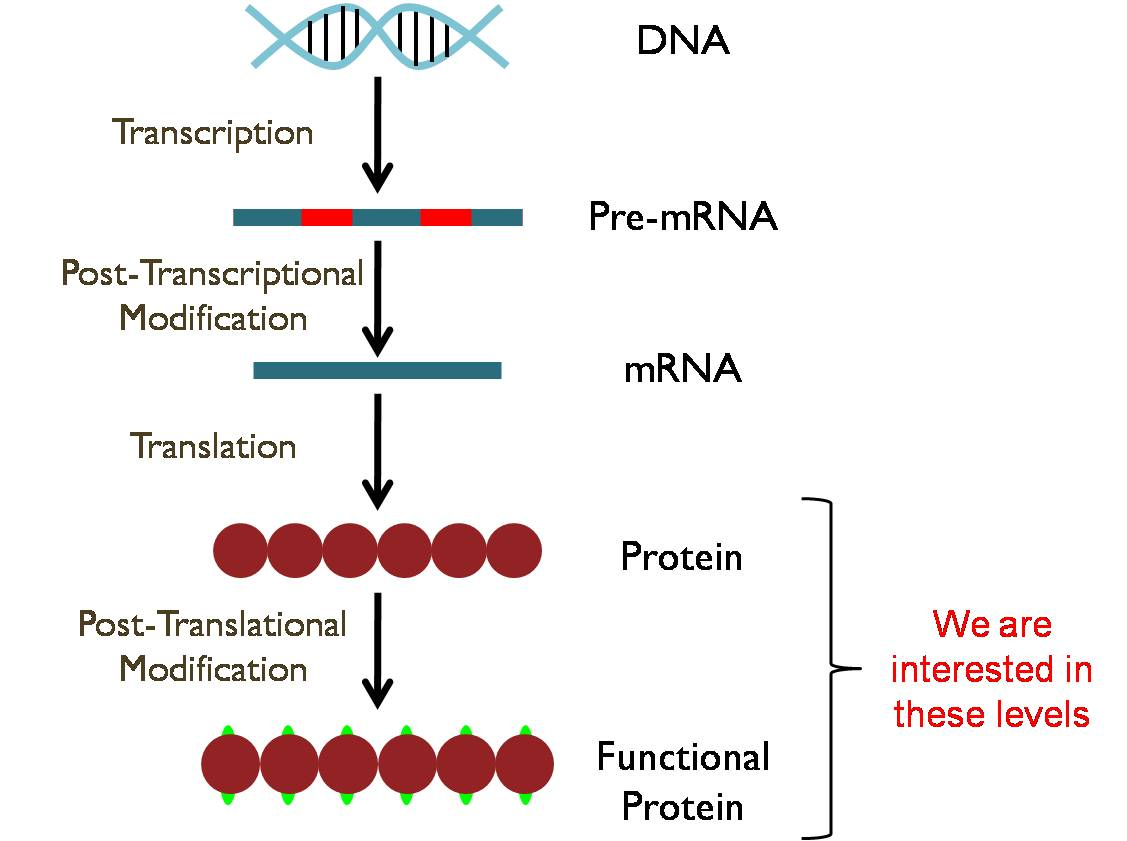
\includegraphics[scale=0.55]{image/processes.jpg}}
\caption{Basic biological processes of producing functional proteins from DNA.}
\label{fig:processes}
\end{figure}

There are many ways to study proteins. For example, physical structures of a protein can be studied by X-ray crystallography~\citep{Blow2002}, protein-protein interactions can be studied using the yeast two-hybrid system~\citep{Fields1989}, and the abundance of an individual protein under a defined condition can be studied using isotopic-labelling. The latter, referred to as \emph{quantitative proteomics}, is achieved via a process of separating a complex protein mixture into smaller subunits to enable high resolution measurements of the constituent components of proteins. The use of  {\bf Mu}lti-dimensional {\bf P}rotein {\bf I}dentification {\bf T}echnology (MudPIT) together with {\bf i}sobaric {\bf T}ags for {\bf R}elative and {\bf A}bsolute {\bf Q}uantitation (iTRAQ$^{\rm TM}$) is just one technology used to measure protein abundance.  

\subsection{Multi-dimensional protein identification technology} \label{subsec:MudPIT}
Multi-dimensional Protein Identification Technology (MudPIT) is a chromatography-based method, which uses a suite of technologies to separate a peptide mixture in order to identify and quantify the constituent proteins in the original sample \citep{Washburn2001}. The process typically involves the separation of the peptide mixture into three orthogonal dimensions. The first separation of peptide species is by their charge, using \emph{strong cation exchange chromatography} (SCX). This is followed by a second separation by hydrophobicity, using \emph{reversed phase liquid chromatography} (RPLC). The third separation is by mass, and is carried out by \emph{mass spectrometry} (MS). The combination of all three separation steps reduces the complexity of the sample and enables high throughput protein analysis. Each MudPIT \emph{run} thus comprises these three steps of separation.

The SCX column contains immobilised negatively charged sulfonic acids that form an ionic interaction with the positively charged peptides. Hence, the charge separation by SCX divides a protein digest (i.e. a mixture of peptides) into many different fractions based on the strength of the charge interaction between the peptides and the sulfonic acids. Different peptide sequences have different affinities for the SCX resin. This allows for complex peptide mixtures to be fractionated by gradually increasing the concentration of a competing salt solution (for binding to the sulfonic acid groups in a gradient) in a step-wise manner. The salt concentration ranges between 10mM to 500mM. Hence, at each interval of salt concentration, a set of peptides is released into the next MudPIT phase. Each of these charge intervals is termed a \emph{salt step}, and increasing the number of salt steps enables the detection of proteins with low abundance. 

The set of peptides from each charge fraction is then separated by RPLC based on hydrophobicity. This is achieved with a separate column that contains silica beads with chains of 18 carbon atoms attached. The peptides are loaded into the column, where they undergo hydrophobic interactions with the carbon chains. An organic solvent is then added to the column in concentrations that increase over time, causing the peptides to emerge or \emph{elute}, with the least hydrophobic peptides eluting first. Eluted peptides are then detected using the mass spectrometer.

The mass analysis is performed by MS, whereby each peptide's \emph{mass-to-charge ratio} (m/z) is measured and then used to calculate its molecular mass. Peptide separation is described in more detail in \cite{Eidhammer2008}. 

\emph{Tandem mass spectrometry} (MS/MS), which consists of two repeated phases of MS, was used for this study. Peptide fragmentation occurs between the two phases of MS, and identification and quantification of the peptides and proteins is thus based on these peptide fragments. MS/MS enables higher specificity in protein identification and enables more accurate quantification.

MudPIT has some limitations. For example, large variation in signal intensity between different MudPIT runs can make inter-sample comparisons of peptide or protein abundance difficult. This limitation has been resolved by iTRAQ$^{\rm TM}$ labelling, which enables the simultaneous analysis of up to eight distinct protein digests within a single MudPIT run. For this thesis, each MudPIT run is referred to as a \emph{run}. 

\subsection{iTRAQ$^{\rm TM}$ for protein quantitation}\label{subsec:iTRAQ}
In 2004, \citeauthor{Ross2004} introduced a peptide labelling technology, namely isobaric Tags for Relative and Absolute Quantitation (iTRAQ$^{\rm TM}$), enabling differential labelling of peptides in different biological samples. In its initial format, iTRAQ$^{\rm TM}$ comprised four isobaric tags, each consisting of a reporter group, a balance group, and a peptide reactive group. The reactive group binds the N-terminus at the start of each peptide, and, for those peptides contain lysine residues (i.e. amino acid), then also on the lysine's side chain. The four reporter groups have m/z values 114, 115, 116 and 117, with corresponding balance group values of 31, 30, 29 and 28. Each of the four tags thus has an identical total m/z value of 145 Da, making them isobaric. This enables identical peptide species, differentially labelled with the four tags, to be indistinguishable with respect to the intact mass of the peptide when selected for MS/MS~\citep{Ross2004}. For MS/MS, the relative abundances are determined using the reporter ion signals at m/z values of 114, 115, 116 and 117 on the \emph{mass spectrum}, i.e.\ the graphical representation of the peptides and peptide fragments based on their m/z values and abundances. Mass spectra are generated for both phases of MS/MS, i.e.\ for the intact peptide during the first cycle, and for the fragmented peptides during the second fragmentation cycle. The four different labels thus allow the simultaneous analysis of four different samples ~\citep{Ross2004}.
 
\begin{figure}[!htb]
\centering{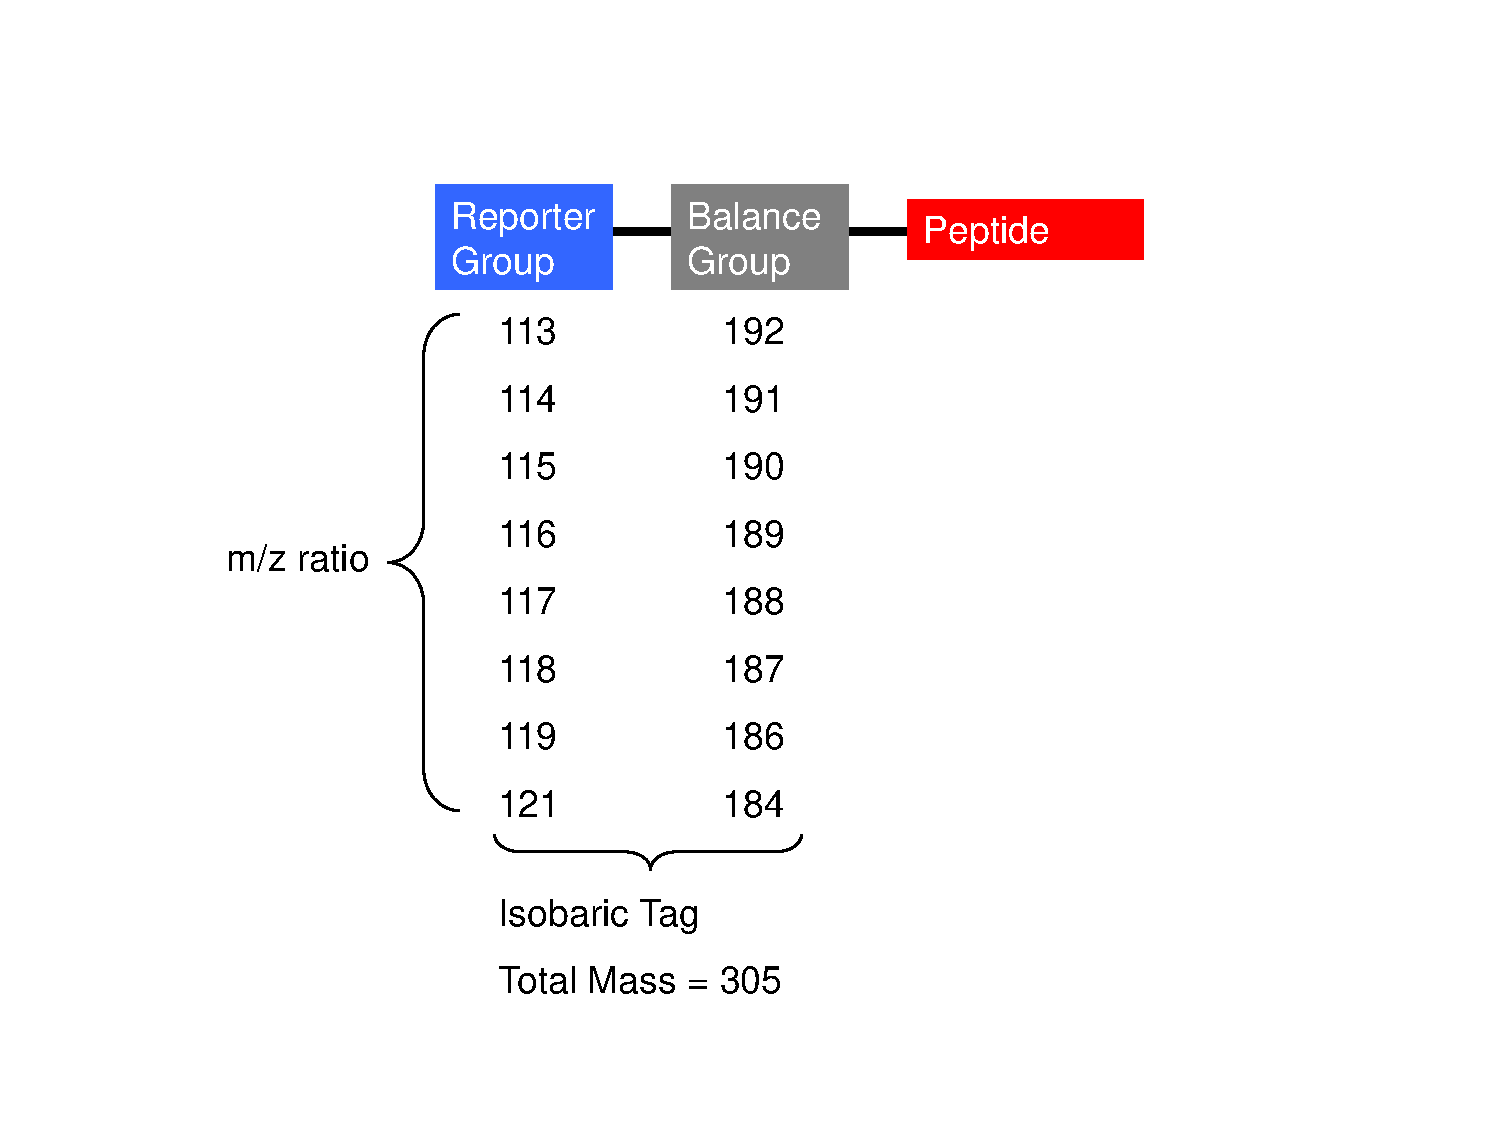
\includegraphics[scale=0.6]{image/iTRAQtags.pdf}}
\caption{Structure of eight-plex-iTRAQ$^{\rm TM}$ tags showing the reporter and balance group masses measured using m/z~\citep{Choe2007}.}
\label{fig:eight-plex}
\end{figure}

\cite{Choe2007} described a new multiplexing strategy, based on the same concept as the four-plex iTRAQ$^{\rm TM}$ system, allowing the simultaneous analysis of up to eight distinct protein samples (see Figure~\ref{fig:eight-plex}). This scheme involves reporter ion signals located at m/z values of 113, 114, 115, 116, 117, 118, 119 and 121. No label is used for an m/z of 120 because it has the same mass as the phenylalanine immonium ion~\citep{Pierce2008}.  For this thesis, each iTRAQ$^{\rm TM}$ tag is referred to as a \emph{tag}. 

\subsection{MudPIT coupled with iTRAQ$^{\rm TM}$: laboratory workflow}\label{sec:MudPITiTRAQ}
Once the target cells or tissues are harvested, each sample is independently processed, including steps for reduction, alkylation, total protein quantification, and enzymatic digestion (usually with trypsin) into many smaller peptide fragments~\citep{Ross2004}. Since proteins exist in a three-dimensional structure, held together by disulfide bonds, reduction breaks down these bonds to produce a two-dimensional linear structure. The alkylation step prevents the reformation of the disulfide bonds. A protein assay is used to measure the total protein content of each sample after reduction and alkylation. This ensures that the total amount of protein to be compared using iTRAQ$^{\rm TM}$ is approximately equal for all samples. Enzymatic digestion with trypsin specifically cleaves the protein immediately after every lysine (K) and arginine (R) residue (see Figure~\ref{fig:protDigest}). 

\begin{figure}[htb]
\centering{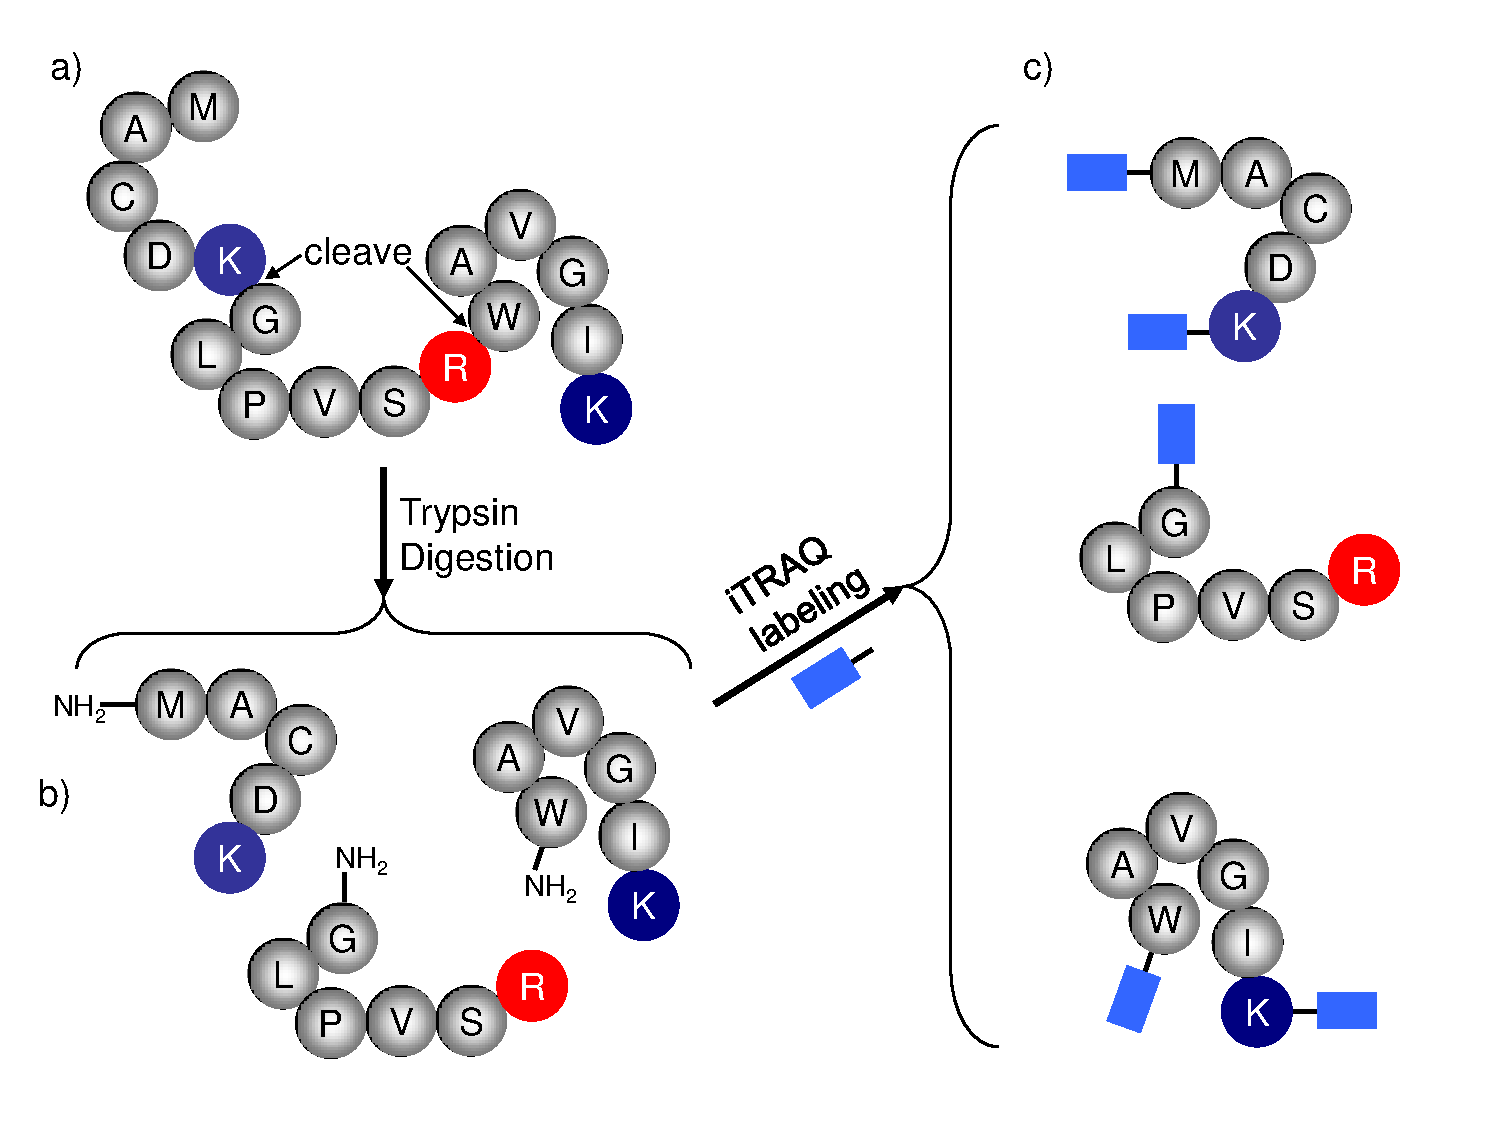
\includegraphics[scale=0.5]{image/proteinDigest.pdf}}
\caption{The process of protein digestion by trypsin. a)Intact protein. b)Digested peptides showing free N-termini. c)Peptides labelled with iTRAQ$^{\rm TM}$ tag.}
\label{fig:protDigest}
\end{figure}

The iTRAQ$^{\rm TM}$ labelling chemistry works by binding the tag to the free N-termini at the start of each peptide and on the K side chain. Thus, with fully efficient enzymatic cleavage, peptides containing one K residue are labelled twice, as the K residue's side-chain also contains a free N-terminus~\citep{Wiese2006}. However, missed cleavages do occur, resulting in some peptides containing more than one K residue. A consequence of this is that these additional K residues are also tagged resulting in a much higher reporter ion abundance due to the additional tags. For example, if a peptide has been labelled twice, the abundance of this peptide is shown as double the true amount in the mass spectrum. To avoid this complication, a \emph{relative quantification} is used instead of an \emph{absolute quantification}. Absolute quantification is calculated as the ratio of a target protein's abundance to a protein of a known concentration either within the same sample, or in a different sample in the same MudPIT run~\citep{Thelen2007}. The sample of known concentration is also referred as a \emph{spike-in}. Relative quantification is the ratio of a particular protein's abundance in one sample to the same protein's abundance in another sample, within the same MudPIT run. Calculating the relative abundance overcomes the issue of the multiple tags on the same peptide because they cancel through this division process. 

Next, approximately equal concentrations of the differentially labelled peptide samples are pooled and undergo the first two phases of MudPIT, i.e. separation by charge with SCX, and separation by hydrophobicity with RPLC (see Section~\ref{subsec:MudPIT}). Finally, the peptide mixture is analysed according to molecular mass using MS/MS. There are many different types of mass spectrometer. An example presented here is the \emph{ElectroSpray Ionisation Quadrupole-Time-Of-Flight tandem mass spectrometer} (ESI-qTOF-MS/MS), called the QSTAR\textsuperscript{\textregistered} (Sciex) (see Figure~\ref{fig:MS/MS}). 
  
\begin{figure}[htb]
\centering{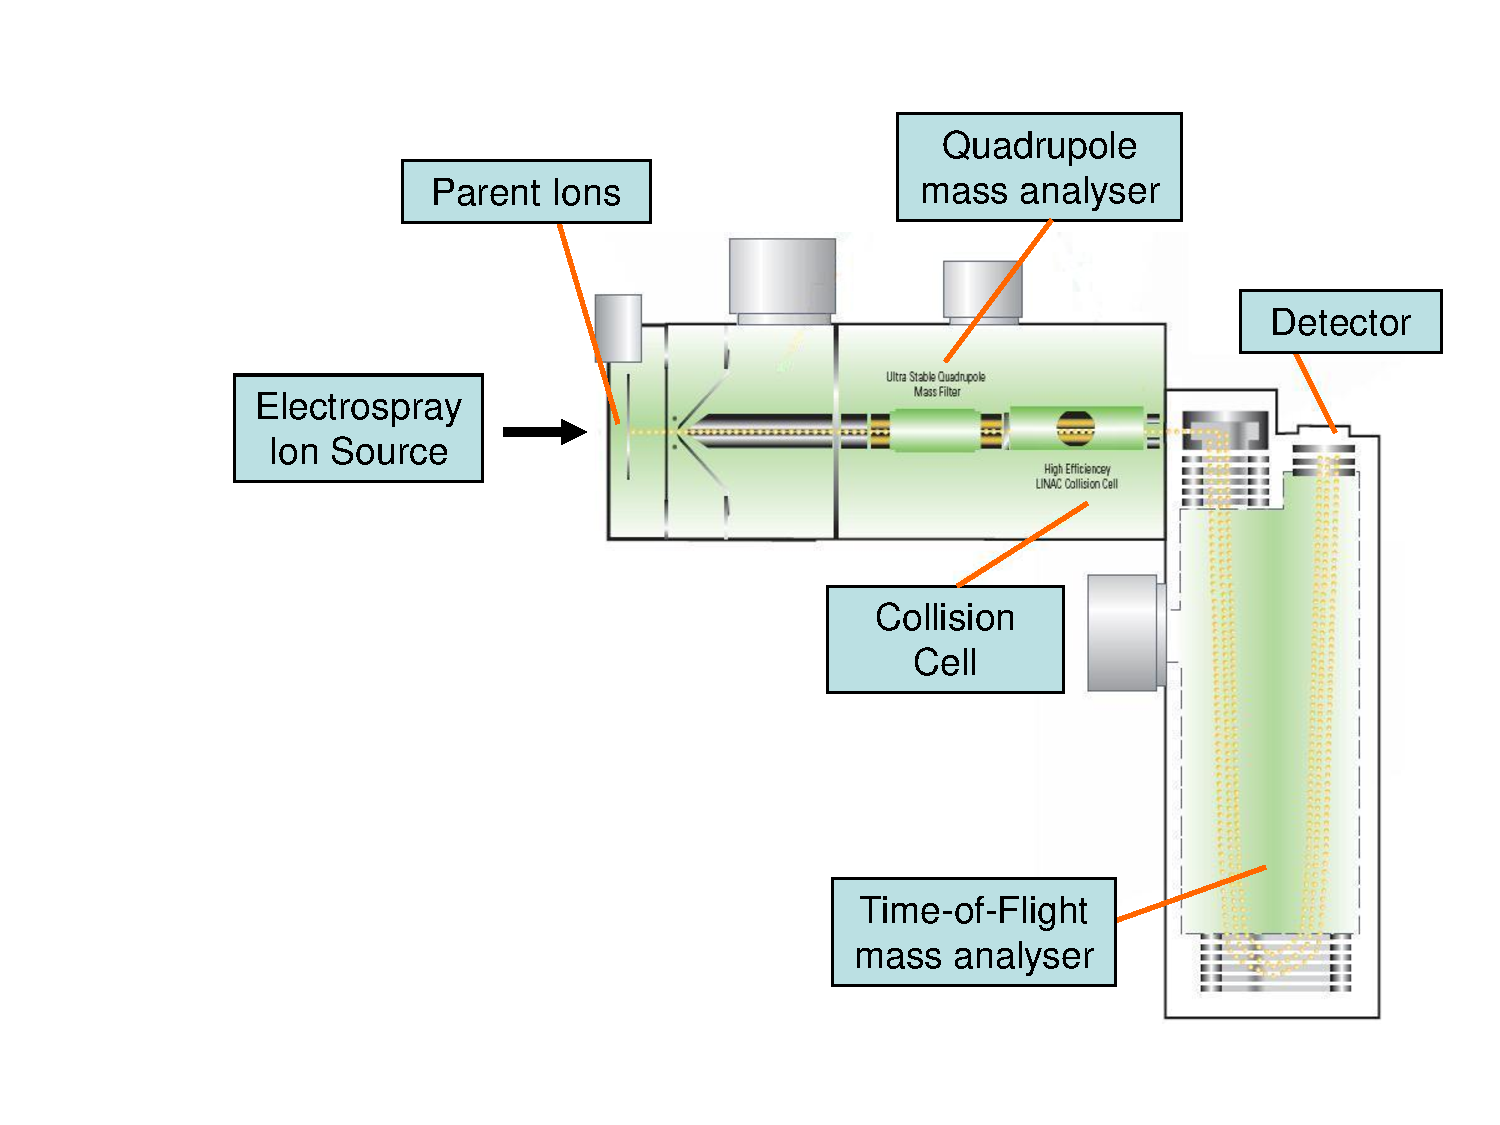
\includegraphics[scale=0.6]{image/qTOF-MSMS.pdf}}
\caption{Schematic of analysis of a protein digest in the QSTAR\textsuperscript{\textregistered} qTOF-MS/MS ~\citep{Applied2004}.}
\label{fig:MS/MS}
\end{figure}

The first step of MS/MS involves subjecting the peptide mixture to ElectroSpray Ionisation (ESI), which transforms each peptide into a positively charged ion, thereby allowing the peptides to be selected, analysed and detected by the mass spectrometer. The separated peptide ions (i.e. ionised peptides) eluting from the RPLC are sprayed continuously into the mass spectrometer for up to 100 minutes for each salt step.   

\begin{figure}[!htb]
\centering{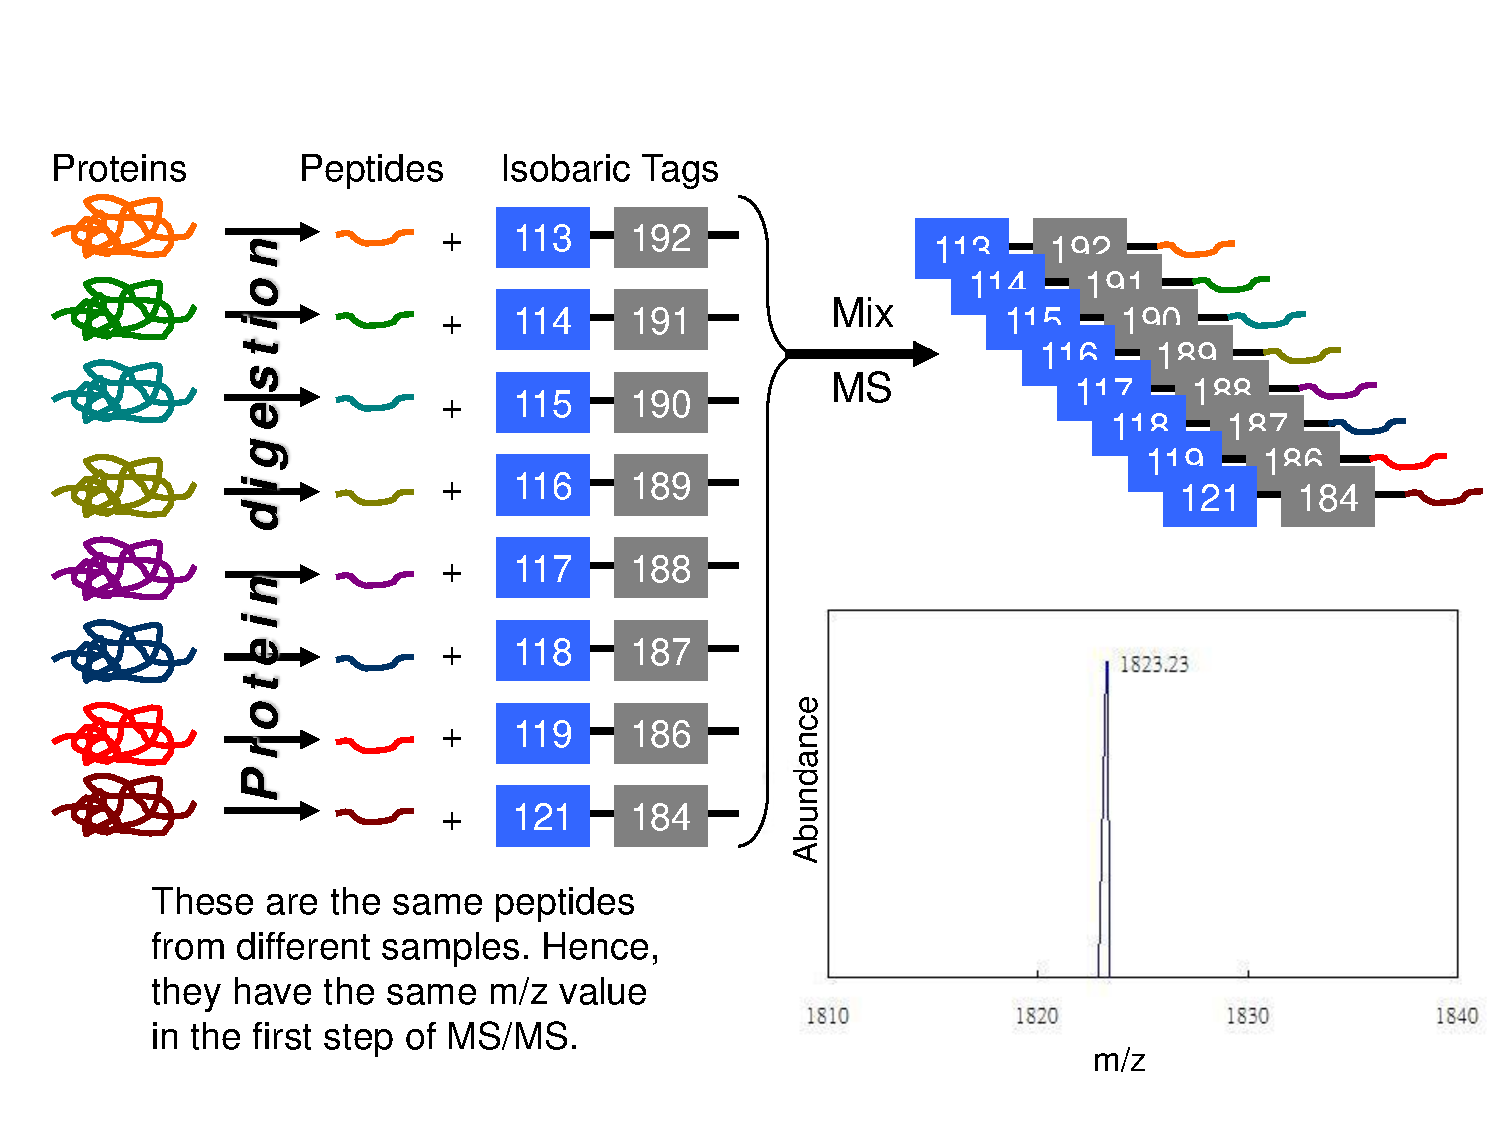
\includegraphics[scale=0.6]{image/MS.pdf}}
\caption{The intensity peak resulting from the mass analysis, of a peptide species with m/z = 1823.23. A single peak is generated for the intact peptide since the mass spectrometer cannot distinguish between the eight samples of origin due to the isobaric tags.}
\label{fig:MS}
\end{figure}

MS/MS consists of two repeated phases of mass analysis and both phases use the Quadrupole-Time-Of-Flight (qTOF) mass analyser. In the first phase, all the peptide ions are passed through the quadrupole mass analyser, and their molecular masses are analysed by the time-of-flight (TOF). The TOF measures the time taken for these ions to travel a known distance. From this, each ion's m/z and abundance is estimated and presented in a MS spectrum (see Figure~\ref{fig:MS}). In the second phase, the peptide ions that have the highest abundance, as detected by the MS, are subsequently isolated by the quadrupole mass analyser. Normally up to three different peptide ions, also known as \emph{precursor} or \emph{parent} ions, are selected in one cycle. Note that these selected peptide ions for the second phase of MS are new peptide ions sprayed by the ESI, as once peptide ions are moved into the TOF they are never recovered. Further, the rate of flow is slow enough that software can instantly inform the quadrupole mass analyser to let a specific peptide pass through. Each of these cycles generally takes around 5.5 seconds: one second to acquire the first MS spectrum, then one, one-and-a-half, and two seconds to acquire the three subsequent MS/MS spectra. Figure~\ref{fig:MSandMSMSspectra} illustrates how the MS and MS/MS spectra are produced under the same time scale, where one MS spectrum will generate the three MS/MS spectra from the three most abundant peptides. 

\begin{figure}[htb]
\centering{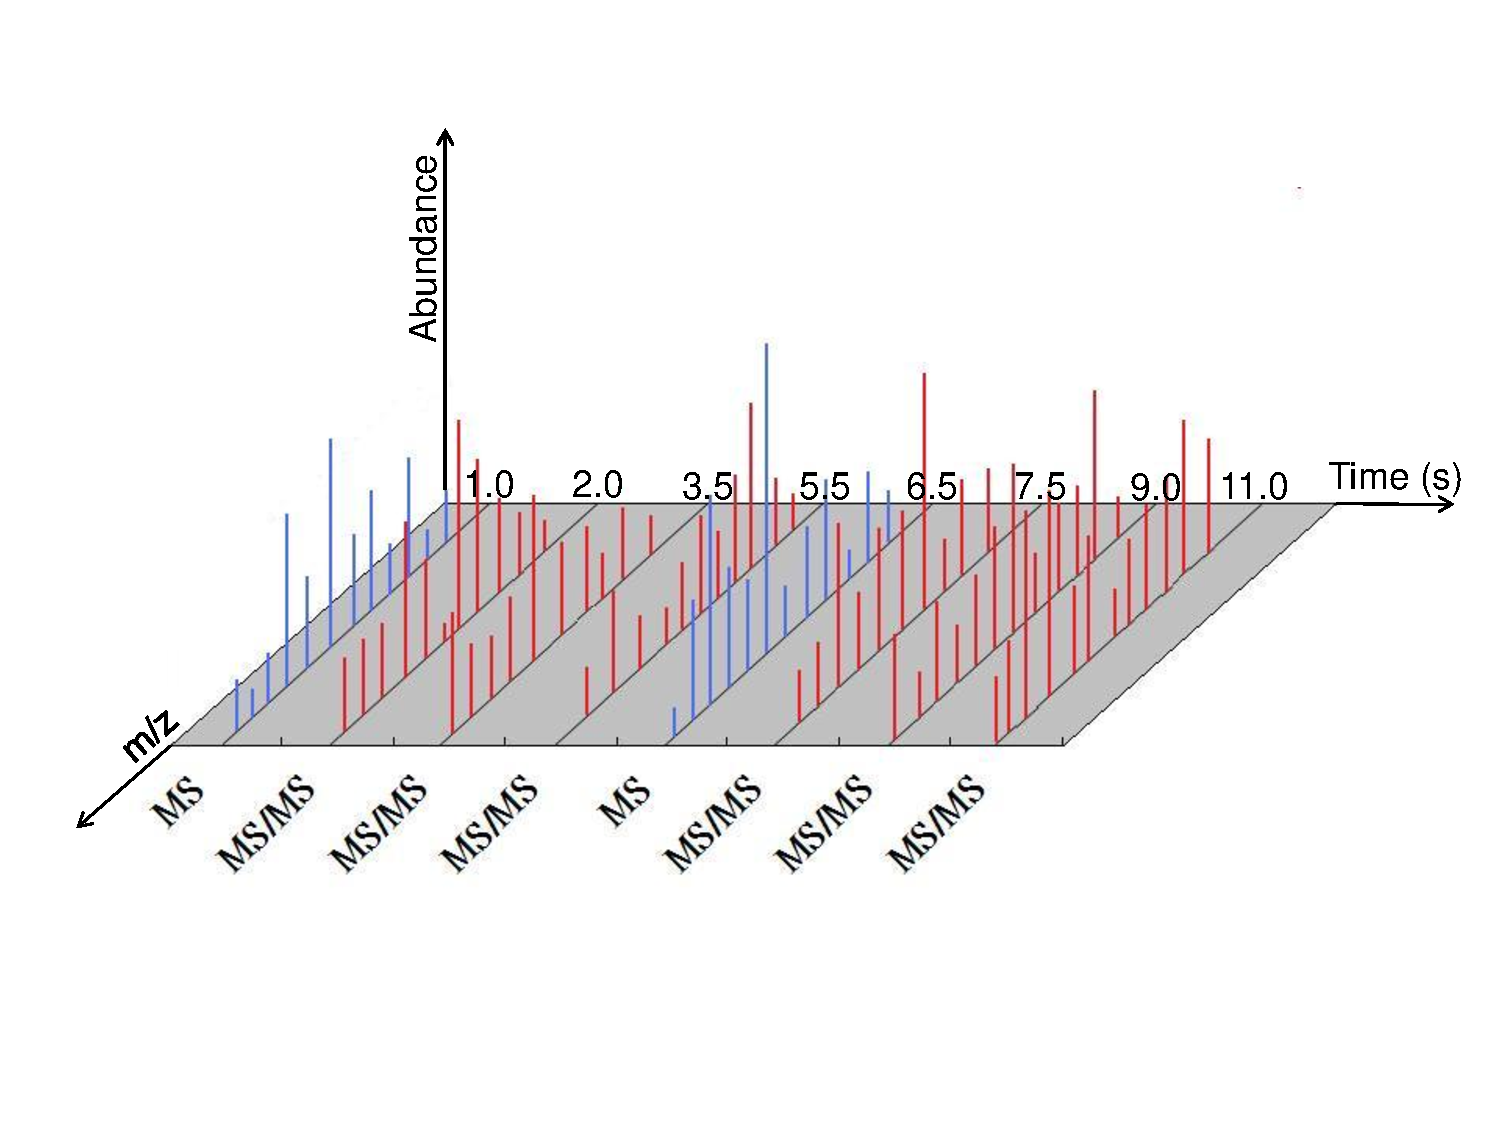
\includegraphics[scale=0.6]{image/MSandMSMSspectra.pdf}}
\caption{Example of MS (blue) and MS/MS (red) spectra.}
\label{fig:MSandMSMSspectra}
\end{figure}

After a specific precursor ion is isolated for the second phase of MS/MS, it moves into a collision cell where it is fragmented into smaller components by collisions with an inert gas. This process, called \emph{collision-induced dissociation} (CID), cleaves the peptide bonds and the chemical bonds with the iTRAQ$^{\rm TM}$ tags. This produces b-ions, y-ions and iTRAQ$^{\rm TM}$ reporter ions (see Figure~\ref{fig:CID}) ~\citep{Ross2004}. The molecular masses of these fragment ions are measured in the TOF. The abundances of the iTRAQ$^{\rm TM}$ labels are estimated from the peaks in the 113 to 121 m/z reporter ion regions. The area under each of these peaks serves as an approximation for the abundance of the peptide in a given sample. The rest of the peaks consist mainly of b- and y- ions, and their m/z are used for peptide identification by comparing the molecular weights of the experimental fragments (i.e. MS and MS/MS spectra) to theoretical fragments generated by in-silico fragmentation of peptides in an appropriate database (see Figure~\ref{fig:spectrum}).

\begin{figure}[!htb]
\centering{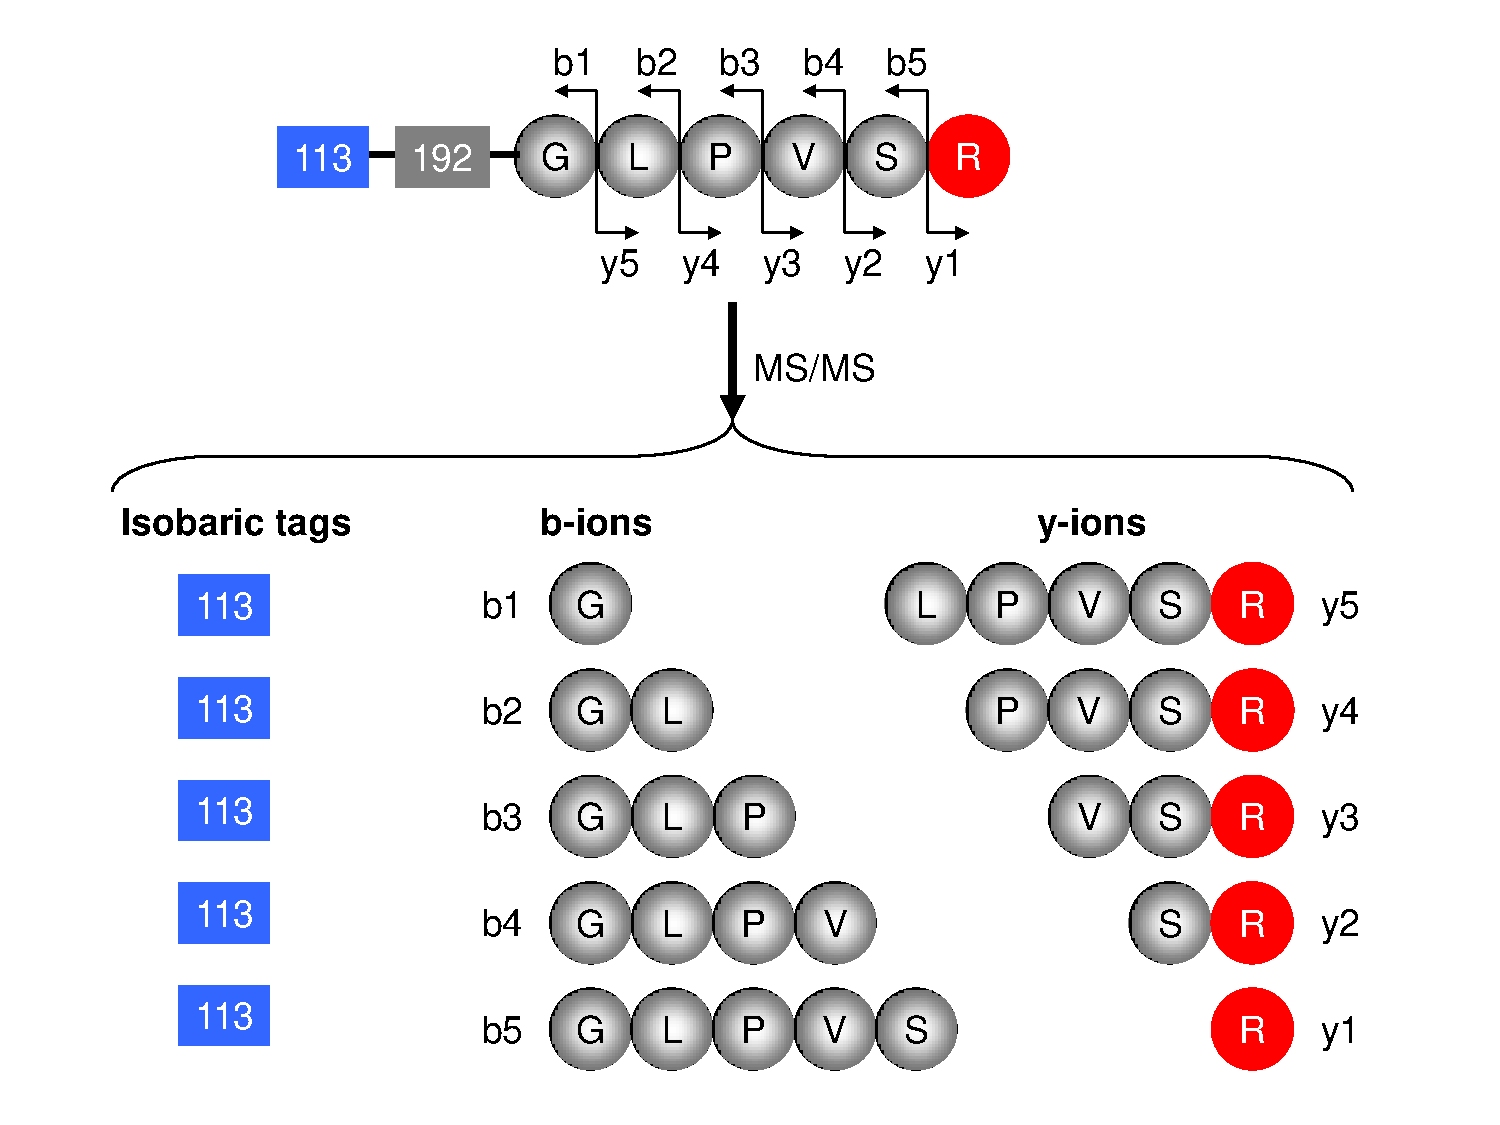
\includegraphics[scale=0.45]{image/CID.pdf}}
\caption{Possible b- and y-ions generated by collision-induced dissociation.}
\label{fig:CID}
\end{figure}

\begin{figure}[!htb]
\centering{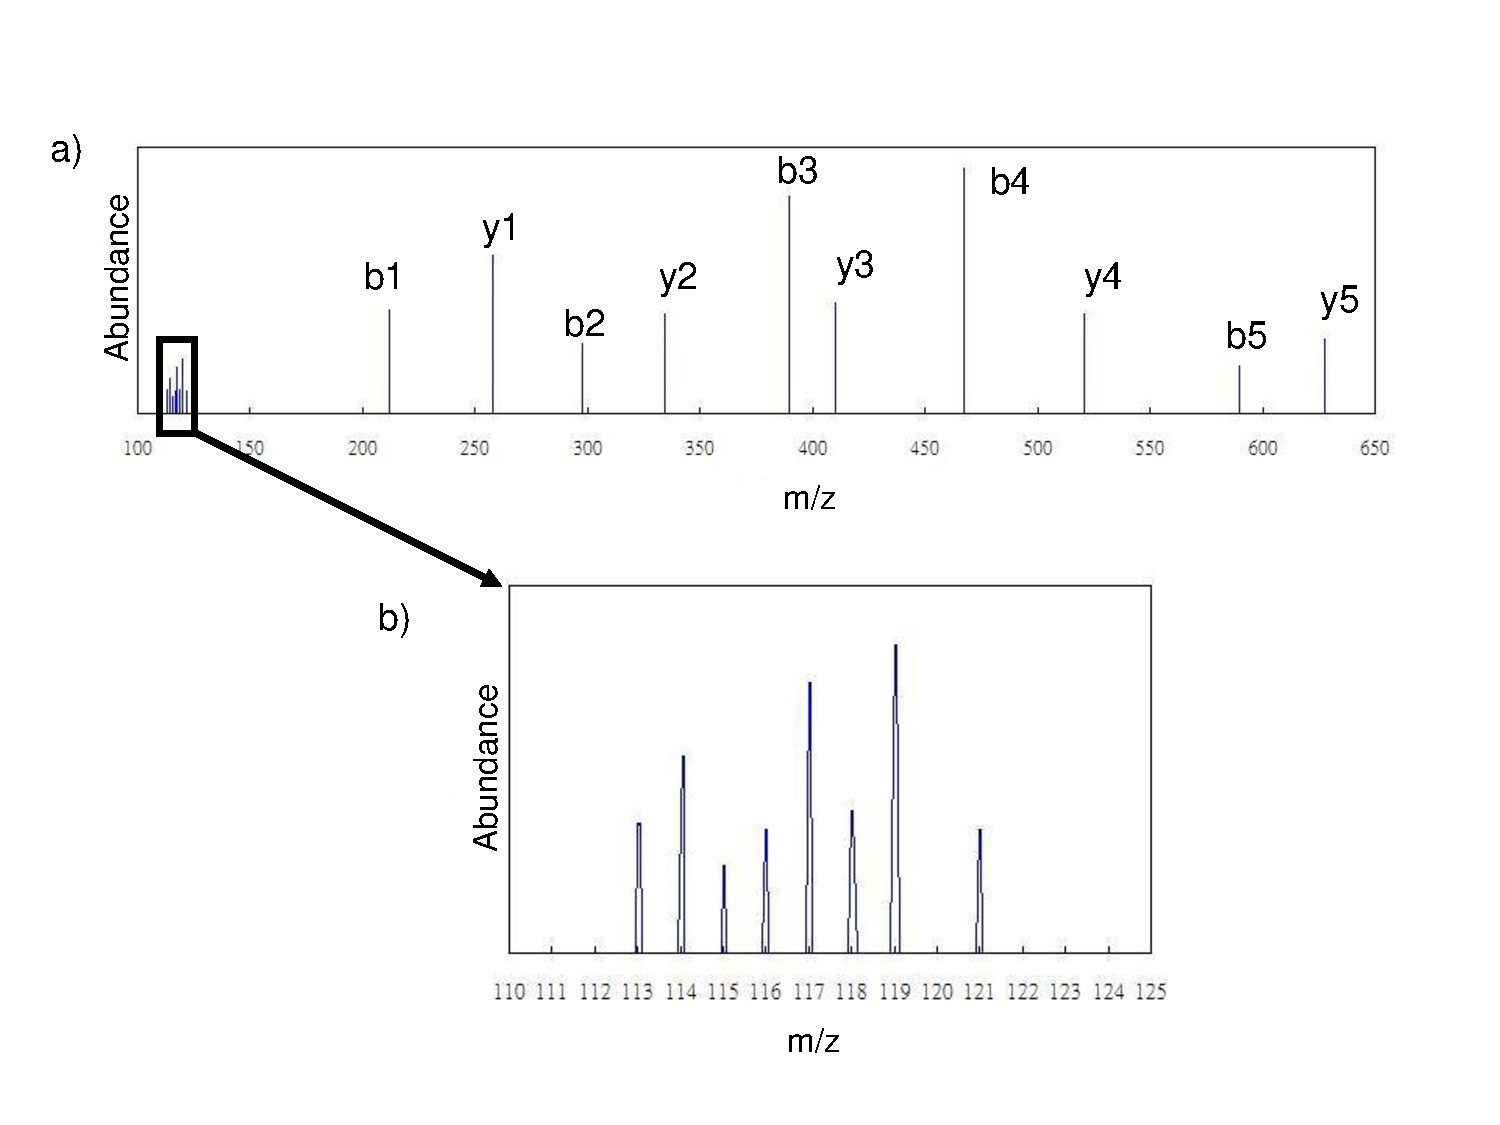
\includegraphics[scale=0.55]{image/mockMSspectra.pdf}}
\caption{a) MS/MS spectra showing the b- and y-ions, and b) zoom-in into 113 to 121 m/z reporter ion region.}
\label{fig:spectrum}
\end{figure}

\subsection{Data generation from MudPIT-iTRAQ$^{\rm TM}$}\label{sec:data}
In every MudPIT run, the QSTAR\textsuperscript{\textregistered} machine generates a WIFF file for each salt step that is performed. Each WIFF file contains all of the MS and MS/MS spectra from the fragmented peptides. There are a number of software packages which are available to perform both peptide-protein identification and the statistical analysis. 

Peptide-to-protein identification involves database searching to identify the proteins that match a given peptide from the MudPIT-iTRAQ$^{\rm TM}$ experimental data. Examples of such software are Mascot$^{\rm TM}$ 2.6 (Matrix Science), SEQUEST\textsuperscript{\textregistered}~\citep{Sadygov2004}, and ProteinPilot$^{\rm TM}$ 5.0 (Sciex). In general, the available software employ a \emph{bottom-up} approach~\citep{Nunn2007}, also known as \emph{shotgun proteomics}~\citep{Nesvizhskii2005}, for protein identification and quantification. The identification method involves a series of peptide matching steps. The mass spectra of the observed fragment ions that were detected in the MudPIT-iTRAQ$^{\rm TM}$ analysis are compared with the mass spectra of theoretical fragment ions, also known as \emph{theoretical spectra}. These theoretical spectra are created from the in-silico tryptic digestion of proteins from an appropriate protein database~\citep{Sadygov2004}. Then, the original intact proteins can be identified from the matched peptides~\citep{Nesvizhskii2005}. 

The database should contain all of the known proteins from a chosen species together with their sequences. Hence, choosing a comprehensive protein sequence database is essential to allow as many peptides as possible to be matched. There are many different protein sequence databases available. The largest and most complete database is Entrez Protein from the National Center for Biotechnology Information (NCBI), because this database is made up of several other databases. However, since this database is generated automatically without any manual correction, some peptide sequences may not be determined correctly. Furthermore, this database has a high degree of sequence redundancy and can slow down the searching process. For a higher quality of sequence annotation, it is more appropriate to use well-curated databases such as Swiss-Prot from the European Bioinformatics Institute (EBI), or Reference Sequence (RefSeq) from NCBI. If the database search cannot find a match for an observed spectrum, then manual peptide sequencing is possible using a process called \emph{de novo peptide sequencing}~\citep{Colinge2007}. Rather than pattern matching the observed spectrum to a theoretical spectrum, de novo peptide sequencing sequences incrementally using the m/z corresponding to the masses of amino acid residues to build the potential sequence of the unknown peptide~\citep{Colinge2007}.

\section{Overview of thesis}
\label{sec:overview}
The primary purpose of this thesis is to develop a method for the computer generation of optimal designs for two-phase multiplex proteomics experiments. This thesis has three parts. The first part, presented in Chapter 2, describes the method of information decomposition of the design in any single- and two-phase experiment, and automates the construction of theoretical ANOVA tables. The second part is the main component of the thesis where we describe a computational approach for finding optimal designs for Phase 2 proteomics experiments. Chapter 3 considers the case of the Phase 1 experiment arranged in a completely randomised design and Chapter 4 considers the case of the Phase 1 experiment arranged in a randomised complete block design (RCBD), or a balanced incomplete block design (BIBD). The third part, presented in Chapter 5, shows how to estimate the variance components and the effective degrees of freedom (EDF) using the restricted maximum likelihood (REML). The comparison of some optimal designs found in Chapters 3 and 4 using the EDF can help clarify the properties of different candidate designs. Chapter 6 summarises and concludes the entire thesis. Furthermore, it presents future directions in the design and analysis of two-phase experiments, in particular, for quantitative high-throughput biotechnology experiments with multiplexing technology. These technologies are currently useful and will remain so for the next decade.


%\bibliographystyle{apalike}
%\bibliography{ref}

%\end{document}

\include{Chapter2/computeVC}
\include{Chapter3/rcdOptDesign}
\include{Chapter4/rbdOptDesign}
\chapter{Estimation of variance components and effective degrees of freedom in two-phase proteomic experiments}

\section{Introduction}
\label{sec:introChap5}
In Chapter 2, we described the methodology needed to construct theoretical ANOVA tables for two-phase experiments. Chapters 3 and 4 then developed methods for constructing and searching for optimal designs for Phase 2 proteomics experiments when the Phase 1 experiment is arranged in a completely randomised design (CRD), a randomised complete block design (RCBD), or a balanced incomplete block design (BIBD). Theoretical ANOVA tables were shown to be a very useful tool for investigating and comparing the properties of optimal designs of different Phase 2 experiments for a given Phase 1 design. This chapter presents a third component of this thesis in estimating variance components (VCs) based on expected mean squares (EMS) of the theoretical ANOVA table, where we focus on the Residual mean squares (MS) of the same stratum for testing the Treatment effects. The example of this chapter is in the Between Animals Within Runs stratum. In addition, the Phase 2 Block (Run) effects are assumed to be random may allow us to obtain a test that effectively has higher degrees of freedom (DF) for the Residual MS, namely the \emph{effective degrees of freedom} (EDF).  

%Consider where a Phase 1 experiment is arranged in a CRD with $s_b = 3$ biological replicates of each of $\nu = 2$ treatments, meaning the total number of animals is 6. If a four-plex system is used, the animals cannot be allocated to runs such that animals effects are orthogonal to run effects. Hence, some animal information is contained in the Between Runs stratum. This chapter aims to show how to recover some of this animal information from the Between Runs stratum, which resulting in higher residual degrees of freedom (DF) for estimating the variances of the treatment effects. This adjusted DF is known as the \emph{effective degrees of freedom} (EDF). 

\cite{Jarrett2008} demonstrated that given the same design at Phase 1, the choice of design at Phase 2 can affect the analysis of a micro-array experiment. MudPIT-iTRAQ$^{\rm TM}$ experiments have their own unique set of problems. Either a four-plex or eight-plex labelling system can be used for the Phase 2 proteomics experiment, which allows researchers to measure either four or eight biological samples simultaneously. The EDF provide us with another property by which we can compare designs using four- and eight-plex systems, which we will apply to some of the optimal designs of the Phase 2 experiments found in Chapters 3 and 4.

%The EDF are computed based on the estimated variance components (VCs). Two methods of estimating VCs are discussed in this chapter. The first method uses a linear combination (LC) of the residual expected mean squares (EMS) from the theoretical ANOVA table. The second method attempts to improve the estimation of VCs using restricted maximum likelihood (REML) \citep{Patterson1971}. The EDF are then computed from the first two moments of an approximate $\chi^2$ distribution using the Satterthwaite approximation \citep{Satterthwaite1946}.
  
This Chapter first uses an optimal design, described in Section~\ref{sec:expDes}, to illustrate the estimation of VCs in Section~\ref{sec:estVC}. Based on the VCs estimates, the approximation method for the EDF is then shown in Section~\ref{sec:estEDF}. Section~\ref{sec:expCRD} compares the EDF between the Phase 2 design with four-plex and eight-plex systems given the same Phase 1 experiment arranged in a CRD. Section~\ref{sec:expRCBD} compares the EDF between four Phase 2 designs, given the same Phase 1 experiment is arranged in a RCBD, using two different confounding schemes when the Phase 1 Block effects are intentionally confounded with Tag effects or Phase 1 Block effects are intentionally confounded with Run effects, and between the four-plex and eight-plex systems.   

\section{An illustrative example}
\label{sec:expDes}
This section presents the most trivial example of a two-phase experiment, in which the Phase 1 experiment is arranged in a CRD with $\nu = 2$ treatments assigned to $n_a = 6$ animals. The layout of the Phase 1 design consists of Treatment \textit{a} assigned to Animals \textit{A}, \textit{C} and \textit{E}, and Treatment \textit{b} assigned to Animals \textit{B}, \textit{D} and \textit{F}. The samples from each animal are further split into $n_s$ sub-samples which are differentially labelled by $n_\gamma$ tags and analysed in $n_r$ runs of the Phase 2 experiment. The linear model of this Phase 2 experiment has been previously described in (\ref{eq:model}). 

\begin{table}[ht]
\centering
\itshape
\caption{Optimal design of Phase 2 proteomics experiment showing allocation of sub-samples from animals and treatment to runs and tags, when the Phase~1 experiment consists of $\nu = 2$ treatments assigned to each of $n_a = 6$ animals, $n_s = 2$ sub-samples are then taken from each animal, and labelled by $n_\gamma = 4$ tags and analysed in $n_r = 3$ runs of the Phase 2 MudPIT-iTRAQ$^{\rm TM}$ experiment.}
\begin{tabular}{c|cc:cc}
 & \multicolumn{4}{c}{{\bf Tag}} \\
{\bf Run}  & \textnormal{114} & \textnormal{115} & \textnormal{116} & \textnormal{117} \\ 
\hline 
\textnormal{1} & Db & Ca & Fb & Ea \\  
\textnormal{2} & Ca & Db & Ea & Fb \\  \hdashline
\textnormal{3} & Bb & Bb & Aa & Aa \\ 
\end{tabular} 
\label{tab:aniDes1Chap5}
\end{table}

An optimal design found using the methods described in Chapter 3 is shown in Table~\ref{tab:aniDes1Chap5}. There are several characteristics of this design: Runs 1 and 2 contain sub-samples from Animals $C$, $D$, $E$ and $F$, while Run 3 contains sub-samples from Animals $A$ and $B$. Thus, 1 of 4 DF associated with the Animal effects is confounded with 1 DF of the Between Runs stratum. Furthermore, Animals $B$, $C$ and $D$ are assigned to Tags 114 and 115, and Animals $A$, $E$ and $F$ are assigned to Tags 116 and 117. Thus, 1 DF associated with Tag effects is in the Between Animals stratum. Treatment effects are orthogonal to Run effects, as each run contains two of each treatment. There are unequal numbers of sub-samples from Treatment \textit{a} and \textit{b} labelled with each Tag resulting in some confounding between Treatment and Tag effects.

\begin{table}[ht]
\centering
\caption{Theoretical ANOVA table of the Phase 2 experiment in Table~\ref{tab:aniDes1Chap5}.}
\begin{tabular}{lrllll} 
\toprule 
\multicolumn{1}{l}{\textbf{Source of Variation}} & \multicolumn{1}{l}{\textbf{DF}}& \multicolumn{1}{l}{\textbf{MS}} & \multicolumn{1}{l}{\textbf{EMS}}& \multicolumn{1}{l}{$\bm{E_{\gamma}}$}&\multicolumn{1}{l}{$\bm{E_{\tau}}$}\\ 
\midrule 
Between Runs & & &  & & \\ 
\quad Between Animals & $1$ &$s_1^2$ & $ \sigma^2+2\sigma_{a}^2+4\sigma_{r}^2$ & & \\ 
\quad Within Animals & $1$ &$s_2^2$& $\sigma^2+4\sigma_{r}^2$ & & \\ \hline 
Within Runs &  &&  & & \\ 
\quad Between Animals &&  &  & & \\ 
\quad \quad Tag & $1$ && $\sigma^2+2\sigma_{a}^2+3\theta_{\gamma}+0.67\theta_{\tau}$ &$1$ & $0.111$\\ 
\quad \quad Treatment & $1$ & & $\sigma^2+2\sigma_{a}^2+5.33\theta_{\tau}$ & & $0.889$\\ 
\quad \quad Residual & $2$ &$s_3^2$& $\sigma^2+2\sigma_{a}^2$ & & \\ \hline 
\quad Within Animals &  &&  & & \\ 
\quad \quad Tag & $2$ && $\sigma^2+3\theta_{\gamma}$ &$1$ & \\ 
\quad \quad Residual & $3$ &$s_4^2$& $\sigma^2$ & & \\ 
\bottomrule 
\end{tabular} 
\label{tab:Phase2ANOVAChap5} 
\end{table} 

The theoretical ANOVA of the optimal design of the Phase 2 experiment in Table~\ref{tab:aniDes1Chap5} is presented in Table~\ref{tab:Phase2ANOVAChap5}. Notice that an additional column is present in this table, namely the mean square (MS) column, i.e.\ the estimated value of its corresponding EMS being computed from experimental data. There are four MS of interest, which contain only the random error variances: the Between Animals Between Runs MS ($s_1^2$), the Within Animals Between Runs MS ($s_2^2$), the Residual MS of the Between Animals Within Runs stratum ($s_3^2$) and the Residual MS of the Within Animals Within Runs stratum ($s_4^2$). These MS, also known as residual variances, are related to their associated EMS as follows 
\begin{eqnarray}
\label{eq:s1} s_1^2 &=&  \hat{\sigma}^2+2\hat{\sigma}_{a}^2+4\hat{\sigma}_{r}^2,\\
\label{eq:s2} s_2^2 &=&  \hat{\sigma}^2+4\hat{\sigma}_{r}^2,\\
\label{eq:s3} s_3^2 &=&  \hat{\sigma}^2+2\hat{\sigma}_{a}^2,\\
\label{eq:s4} s_4^2 &=&  \hat{\sigma}^2,
\end{eqnarray}
where $\hat{\sigma}^2$, $\hat{\sigma}_{a}^2$, and $\hat{\sigma}_{r}^2$ are the estimated between sub-samples, between animals, and between runs VCs, respectively. The $\hat{\sigma}^2$ is the residual variance from the Within Animals Within Runs stratum as shown in (\ref{eq:s4}). Subtracting (\ref{eq:s4}) from (\ref{eq:s3}) gives $\hat{\sigma}_{a}^2 = (s_3^2 - s_4^2)/2$. We then subtract (\ref{eq:s4}) from (\ref{eq:s2}) to solve for $\hat{\sigma}_{r}^2$, which gives $\hat{\sigma}_{r}^2 = (s_2^2 - s_4^2)/4.$ Following \cite{Jarrett2008}, this method of solving a system of linear equations to obtain estimates of the variance components is, from this point forward, referred to as the linear combination (LC) method. 

A purpose of constructing the theoretical ANOVA table is that it enables us to determine variances of Treatment effects, and therefore, a valid F-test for the Treatment effects can be obtained. The estimated Treatment difference between Treatments $a$ and $b$ is given by $(\bar{y}_{...}^{a..} - \bar{y}_{...}^{b..})$, which, for the Phase 2 design presented in Table~\ref{tab:aniDes1Chap5}, has variance 
\begin{equation}\label{eq:varTrt}
\operatorname{Var}(\bar{y}_{...}^{a..} - \bar{y}_{...}^{b..}) = \dfrac{\sigma^2+2\sigma_{a}^2}{3},
\end{equation}
where $\bar{y}_{...}^{i..}$ denotes the mean of the log-protein abundance values over all observations of Treatment $i$. The denominator of (\ref{eq:varTrt}) is 3, because each treatment group is replicated six times (with two sub-samples from each of three animals). The numerator of (\ref{eq:varTrt}), i.e.\ $\sigma^2+2\sigma_{a}^2$, can be estimated directly from the residual variance in the Within Animals Within Runs stratum, the same stratum in which the Treatment effects are being estimated. 

If Run effects are regarded as fixed effects, the row of Table~\ref{tab:Phase2ANOVAChap5} containing $\sigma_r^2$ is not available to be used, i.e.\ $s_1^2$ and $s_2^2$, which implies that the estimate of variance of the Treatment effects will be based solely on $s_3^2$ with 2 DF. If the Run effects are assumed to be random effects, we can recover extra information about $\sigma_a^2$ from $s_1^2$, defined in (\ref{eq:s1}), as well as information about $\sigma^2$ in the other residual variances. Thus, we can then improve the estimate of $\hat{\sigma}^2+2\hat{\sigma}_{a}^2$ either via the LC method as illustrated above, or by using restricted maximum likelihood (REML) approach to estimate the VC. How this may be achieved is discussed in Section~\ref{sec:estVC}.

\section{Estimation of variance components}
\label{sec:estVC}
The theoretical ANOVA in Table~\ref{tab:Phase2ANOVAChap5} identified four MS, with expected values $\xi_i^2$ and $\upsilon_i$ DF ($i = 1,\dots,4$), which are available for estimation of the VCs defined by $\bm{\varsigma} = (\hat{\sigma}^2, \hat{\sigma}_a^2, \hat{\sigma}_r^2)'$. This section shows the REML approach in estimating the VCs developed by \cite{Jarrett2008}. 

\subsection{Constructing the score function and Fisher information matrix} 
The mean squares $s_i^2$ are assumed to have a $\chi^2$ distribution, i.e.\
\begin{equation}\label{eq:chiDistr}
s_i^2 \sim \dfrac{\xi_i^2}{\upsilon_i} \chi_{\upsilon_i}^2, \;  (i = 1,\dots,4), 
\end{equation}
where $\upsilon_i$ denotes the DF corresponding to $s_i^2$. The log-likelihood of $s_i^2$ can be shown to be 
\begin{equation}\label{eq:logLike}
L(\xi_i^2;s_i^2) =  \operatorname{constant} - \sum_{i = 1}^{4}\left[ \dfrac{\upsilon_i  \log(\xi_i^2)}{2} + \dfrac{\upsilon_i s_i^2}{2\xi_i^2}\right], \;  (i = 1,\dots,4).
\end{equation}  
The score is the first derivative of the log-likelihood function with respect to the $i$th element of EMS, $\xi_i^2$, i.e.\
\[\dfrac{\partial L(\xi_i^2;s_i^2)}{\partial \xi_i^2} = \dfrac{\upsilon_i (s_i^2 - \xi_i^2)}{2\xi_i^4}, \;  (i = 1,\dots,4).\]
Since the expected values vector $\bm{\xi^2}$ is a vector containing $(\xi_1^2, \xi_2^2,\xi_3^2,\xi_4^2)'$, the score function with respect to $\bm{\xi^2}$ can be re-written in vector form as follows
\begin{equation}\label{eq:scoreFunOld}
S(\bm{\xi^2}) = \dfrac{\partial L(\bm{\xi^2};\bm{s^2})}{\partial \bm{\xi^2}} = 
\begin{pmatrix}               
\vspace{8pt}\dfrac{\upsilon_1 (s_1^2 - \xi_1^2)}{2\xi_1^4} \\
\vspace{8pt} \dfrac{\upsilon_2 (s_2^2 - \xi_2^2)}{2\xi_2^4} \\
\vspace{8pt} \dfrac{\upsilon_3 (s_3^2 - \xi_3^2)}{2\xi_3^4}  \\
\vspace{8pt} \dfrac{\upsilon_4 (s_4^2 - \xi_4^2)}{2\xi_4^4}  \\
\end{pmatrix}.
\end{equation}

The Fisher information is defined as the variance of the score, which is computed from the negative of the expectation of the second derivative of the log-likelihood function with respect to $\xi_i^2$. This is also known as the expected Fisher information.

Since the expected values vector $\bm{\xi^2}$ is a vector containing $(\xi_1^2, \xi_2^2,\xi_3^2,\xi_4^2)'$, the negative expectation of the second partial derivative of the log-likelihood function gives a $4 \times 4$ Fisher information matrix, i.e.\
\[  \operatorname{E} \left(-\dfrac{\partial^2 L(\bm{\xi^2};\bm{s^2})}{\partial \bm{\xi^4}}\right) =  \operatorname{E}\left( -
\begin{bmatrix}            
\vspace{8pt} \dfrac{\partial^2 L}{\partial \xi_1^4} &  \dfrac{\partial^2 L}{\partial \xi_1^2\partial \xi_2^2} &  \dfrac{\partial^2 L}{\partial \xi_1^2\partial \xi_3^2} & \dfrac{\partial^2 L}{\partial \xi_1^2\partial \xi_4^2}  \\ 
\vspace{8pt} \dfrac{\partial^2 L}{\partial \xi_2^2\partial \xi_1^2} & \dfrac{\partial^2 L}{\partial \xi_2^4} &  \dfrac{\partial^2 L}{\partial \xi_2^2\partial \xi_3^2} & \dfrac{\partial^2 L}{\partial \xi_2^2\partial \xi_4^2} \\
\vspace{8pt} \dfrac{\partial^2 L}{\partial \xi_3^2\partial \xi_1^2} &  \dfrac{\partial^2 L}{\partial \xi_3^2\partial \xi_2^2} & \dfrac{\partial^2 L}{\partial \xi_3^4} &  \dfrac{\partial^2 L}{\partial \xi_3^2\partial \xi_4^2}  \\
\vspace{8pt} \dfrac{\partial^2 L}{\partial \xi_4^2\partial \xi_1^2} & \dfrac{\partial^2 L}{\partial \xi_4^2\partial \xi_2^2} &  \dfrac{\partial^2 L}{\partial \xi_4^2\partial \xi_3^2} & \dfrac{\partial^2 L)}{\partial \xi_4^4} \\
\end{bmatrix}
\right),  \] 
where $L$ denotes $L(\xi_i^2;s_i^2)$ with the $i$th diagonal element given by
\[\dfrac{\partial^2 L}{\partial \xi_i^4} = -\dfrac{\upsilon_i s_i^2 }{\xi_i^6} + \dfrac{\upsilon_i }{2\xi_i^4},\; ( i = 1, \dots, 4). \]
Its negative has expectation
\[ \operatorname{E} \left( -\dfrac{\partial^2 L}{\partial \xi_i^4} \right) = \operatorname{E} \left(\dfrac{\upsilon_i s_i^2 }{\xi_i^6} - \dfrac{\upsilon_i }{2\xi_i^4}\right) = \dfrac{\upsilon_i  \operatorname{E}(s_i^2) }{\xi_i^6} - \dfrac{\upsilon_i }{2\xi_1^4} =  \dfrac{\upsilon_i  \xi_i^2 }{\xi_i^6} - \dfrac{\upsilon_i }{2\xi_i^4} =  \dfrac{\upsilon_i }{2\xi_i^4}.\] 
The off-diagonal elements of the Fisher information matrix, $\dfrac{\partial^2 L}{\partial \xi_i^2\partial \xi_j^2}$, $(i \neq j)$, are all zero. Thus, it follows that the Fisher information matrix with respect to $\bm{\xi^2}$ is given by 
\begin{equation}\label{eq:fishInfoOld}
\A_{\bm{\xi^2}} =  \operatorname{E} \left(-\dfrac{\partial^2 L(\bm{\xi^2};\bm{s^2})}{\partial \bm{\xi^4}}\right) = \mathrm{diag} \left( \dfrac{\upsilon_i }{2\xi_i^4}\right),\; (i = 1, \dots, 4).
\end{equation}

\subsection{Transformation from expected values in {\boldmath $\xi^2$} to estimates in {\boldmath $\varsigma$}}
The score function and Fisher information matrix, as defined in (\ref{eq:scoreFunOld}) and (\ref{eq:fishInfoOld}), respectively, are functions of $\bm{\xi^2}$. However, the goal here is to estimate the VCs, which this formulation will not allow. Thus, we must first transform the score function and Fisher information matrix to functions of $\bm{\varsigma}$.
 
The relationship between the vector of expected values in $\bm{\xi^2}$ and the vector of VCs estimates in $\bm{\varsigma}$ can be written as 
\[
\bm{\xi^2} = \G \bm{\varsigma},
\]
where the matrix $\G$, has $(i,j)$-th element equal to $\partial \xi_i^2/\partial \varsigma_j$. From the theoretical ANOVA in Table~\ref{tab:Phase2ANOVAChap5}, it follows that the row elements of the $\G$ matrix are the coefficients of the VCs in each Residual EMS, i.e.\
\[\begin{bmatrix}               
1 & 2 & 4\\
1 & 0 & 4\\
1 & 2 & 0\\
1 & 0 & 0\\
\end{bmatrix}.\]
Based on the product rule for differentiation, it follows that 
\begin{equation}\label{eq:gmat}
\dfrac{\partial \bm{\xi^2}}{\partial \bm{\varsigma}} = \G.
\end{equation}
  
Since the log-likelihood in (\ref{eq:logLike}) is a function of $\bm{\xi^2}$ containing four elements, the change of variable technique can be implemented by using the multi-variable chain rule to calculate the score function with respect to $\bm{\varsigma}$, i.e.\ 
\begin{equation}\label{eq:scoreFunLast}
S(\bm{\varsigma}) =\dfrac{\partial L(\bm{\xi^2})}{\partial \bm{\varsigma}} = \dfrac{\partial L(\bm{\xi^2})}{\partial  \bm{\xi^2}} \dfrac{\partial \bm{\xi^2}}{\partial \bm{\varsigma}}, 
\end{equation}
where $ \dfrac{\partial \bm{\xi^2}}{\partial \bm{\varsigma}}$ is the matrix $\G$ defined in (\ref{eq:gmat}). It follows, therefore, the score function with respect to $\bm{\varsigma}$ is
\begin{equation}\label{eq:scoreFunNew}
S(\bm{\varsigma}) = \G' S(\bm{\xi^2})= \G' \dfrac{\partial L(\bm{\xi^2})}{\partial \bm{\xi^2}}
\end{equation}
and the Fisher information matrix with respect to $\bm{\varsigma}$ becomes
\begin{equation}\label{eq:fishInfoNew}
\A_{\bm{\varsigma}} = \G' \A_{\bm{\xi^2}} \G =  \G' \left[\mathrm{diag}\left( \dfrac{\upsilon_i }{2\xi_i^4}\right)\right] \G, \; (i = 1, \dots, 4).
\end{equation}

\subsection{Estimating VCs in {\boldmath $\varsigma^2$}}
Using the score function and the Fisher information matrix defined in (\ref{eq:scoreFunNew}) and (\ref{eq:fishInfoNew}), the vector of VCs, $\bm{\varsigma}$, can be estimated using Fisher's scoring algorithm, which is an iterative procedure that can be used to solve maximum likelihood equations. The formula for Fisher's scoring algorithm can be written as 
\begin{equation}\label{eq:fisherScore}
\bm{\varsigma}_{t+1}= \bm{\varsigma}_t+\A^{-1}_{\bm{\varsigma}_t}S(\bm{\varsigma}_t),
\end{equation}
where $\bm{\varsigma}_{t}$ and $\bm{\varsigma}_{t+1}$ are vectors of VCs estimates at the $t$-th and $(t+1)$-th iterations, respectively. The initial estimates can be any value. The iterations stop when the differences between the VCs estimates in two consecutive iterations are less than $1 \times 10^{-7}$ \citep{Patterson1971}. 

%In the current example, $\bm{\varsigma}^2$ consists of $\sigma^2$, $\sigma_a^2$ and $\sigma_r^2$. The inverses of Fisher information matrix and score function with the function of $\bm{\varsigma}_t^2$ are denoted by $\A^{-1}_{\bm{\varsigma}_t^2}$ and $S(\bm{\varsigma}_t^2 )$, respectively. Thus, to estimate VCs using the Fisher scoring algorithm, the score function and Fisher information matrix need to be defined, and are shown in the remainder of this section. The REML method described here is based on the Fisher's scoring algorithm which is an iterative procedure that can be used to solve maximum likelihood equations. The algorithm can be terminated when the differences between the VCs from two consecutive iterations is less than $1 \times 10^{-7}$ \citep{Patterson1971}. Using the score function and the Fisher information matrix defined in (\ref{eq:scoreFunNew}) and (\ref{eq:fishInfoNew}), the vector of VCs, $\bm{\varsigma}^2$, can be estimated using Fisher's scoring algorithm in (\ref{eq:fisherScore}). The initial estimates can be any value. The iteration will stop when the differences between the VCs estimates of two consecutive iterations are less than $1 \times 10^{-7}$. 


\section{Satterthwaite's approximation in deriving the EDF}
\label{sec:estEDF}
Assessment on how well the estimation of the variance, i.e. $\hat{\sigma}^2+2\hat{\sigma}_{a}^2$, has been performed is by examining the DF of Residual MS associated with the Between Animals Within Runs stratum. Once the VCs are estimated from the experimental data using either the LC or REML method, a higher DF, or EDF, may be approximated. The higher the EDF the better this variance is estimated, and also the higher the Residual DF for the F-test of the Treatment effects. 

Using the estimated VCs, the EDF are approximated as twice the square of the expected mean divided by the variance \citep{Satterthwaite1941}. We can show this based on the mean squares, $s_i^2$, are assumed to have a $\chi_{\upsilon_i}^2$ distribution, from (\ref{eq:chiDistr}), then its expectation is given by
\begin{equation}\label{eq:chiMean}
\operatorname{E}(s_i^2) = \operatorname{E}\left(\dfrac{\xi_i^2}{\upsilon_i}\chi_{\upsilon_i}^2\right) = \dfrac{\xi_i^2}{\upsilon_i} \operatorname{E}(\chi_{\upsilon_i}^2) = \dfrac{\xi_i^2}{\upsilon_i} \upsilon_i = \xi_i^2, 
\end{equation}
and its variance is given by 
\begin{equation}\label{eq:chiVar}
\operatorname{Var}(s_i^2) = \operatorname{Var}\left(\dfrac{\xi_i^2}{\upsilon_i}\chi_{\upsilon_i}^2\right) = \dfrac{\xi_i^4}{\upsilon_i^2} \operatorname{Var}( \chi_{\upsilon_i}^2) = 2 \dfrac{\xi_i^4}{\upsilon_i^2}  \upsilon_i = 2 \dfrac{\xi_i^4}{\upsilon_i}. 
\end{equation}
From (\ref{eq:chiMean}) and (\ref{eq:chiVar}), the EDF are approximated from the twice the square of the expected mean divided by the variance, i.e.\
\[
\operatorname{EDF} = \dfrac{2[\operatorname{E}(s_i^2)]^2}{\operatorname{Var}(s_i^2)} =  \frac{2\xi_i^4}{\dfrac{2\xi_i^4}{\upsilon_i}} =  \upsilon_i.
\]
From Table~\ref{tab:Phase2ANOVAChap5}, the MS of interest is the Residual MS in the Between Animals Within Runs stratum, i.e.\ $s_3^2$, thus the EDF associated with this MS are computed as 
\begin{equation}\label{eq:edf1}
\operatorname{EDF} = \frac{2(s_3^2)^2}{\operatorname{Var}(s_3^2)} = \frac{2(\hat{\sigma}^2 + 2\hat{\sigma}_a^2)^2}{\operatorname{Var}(\hat{\sigma}^2 + 2\hat{\sigma}_a^2)}.
\end{equation}
  
The asymptotic variance of the estimates of $\bm{\varsigma}$ is given by the inverse of the Fisher information matrix, which can be expressed as 
\begin{equation}\label{eq:invFisher}
\A^{-1}_{\bm{\varsigma}} = 
\begin{pmatrix}            
\vspace{8pt}  \operatorname{Var}(\sigma^2) &  \operatorname{Cov}(\sigma^2,\sigma_a^2) &  \operatorname{Cov}(\sigma^2,\sigma_r^2)  \\ 
\vspace{8pt} \operatorname{Cov}(\sigma^2,\sigma_a^2) &  \operatorname{Var}(\sigma_a^2) &  \operatorname{Cov}(\sigma_a^2,\sigma_r^2) \\
\vspace{8pt} \operatorname{Cov}(\sigma^2,\sigma_r^2) &  \operatorname{Cov}(\sigma_a^2,\sigma_r^2) &  \operatorname{Var}(\sigma_r^2)   \\
\end{pmatrix}. 
\end{equation}
The estimated variance of $\sigma^2 + 2\sigma_a^2$ in (\ref{eq:edf1}), i.e.\ $\operatorname{Var}(\hat{\sigma}^2 + 2\hat{\sigma}_a^2)$ is given by the sum of the four elements in the top left $2\times2$ submatrix in (\ref{eq:invFisher}) and can be written as  
\[
\operatorname{Var}(\hat{\sigma}^2 + 2\hat{\sigma}_a^2) = \operatorname{Var}(\hat{\sigma}^2) + 4\operatorname{Var}(\hat{\sigma}_a^2) + 4\operatorname{Cov}(\hat{\sigma}^2,\hat{\sigma}_a^2).
\]  
From (\ref{eq:edf1}), the EDF of Residual MS in the Between Animals Within Runs stratum in Section~\ref{sec:expDes} can be computed from 
\[
\operatorname{EDF} = \dfrac{2(\hat{\sigma}^2 + 2\hat{\sigma}_a^2)^2}{\operatorname{Var}(\hat{\sigma}^2) + 4\operatorname{Var}(\hat{\sigma}_a^2) + 4\operatorname{Cov}(\hat{\sigma}^2,\hat{\sigma}_a^2)}.
\]

\subsection{Comparing VCs between LC and REML methods}
In this section, a simulation study, is used to compare the effects of the two VC estimation methods - LC and REML - on the estimated EDF of the variance, i.e. $\hat{\sigma}^2+2\hat{\sigma}_{a}^2$, for the design in the example discussed in Section~\ref{sec:expDes}. The simulation datasets were generated on the basis that the residual MS have a chi-square distribution, with the ratio of the Between Animals VC to measurement error VC, denoted by $\sigma_a^2/\sigma^2$, set with 17 values ranging from $10^{-4}$ to $10^4$, and the ratio of Between Runs VC to measurement error, denoted by $\sigma_r^2/\sigma^2$, set to $0, 0.25, 1, 5, 100$. The case when run effects of run are fixed is also considered (effectively when $\sigma _r^2 = \infty$). 

Figure~\ref{fig:EDFadjusted} shows the EDF for the range of values of the ratio $\sigma_r^2/\sigma^2$ and $\sigma_a^2/\sigma^2$, including a line for the fixed Run effects case. It shows that the EDF can be as low as 2 DF when there are large Run effects, but that the EDF approach 3 when the between-animal variation dominates. Note that, when the run-to-run variation is substantially larger than the between animal variation we see that the EDF based on VCs estimated using the LC method are slightly higher than those using REML. This suggests that the optimal design presented in Section~\ref{sec:expDes} may be robust to the method of VCs estimation. We will show EDF approximated from both LC and REML methods for the remaining of this Chapter to confirm this. 

\begin{figure}[ht]
\centering
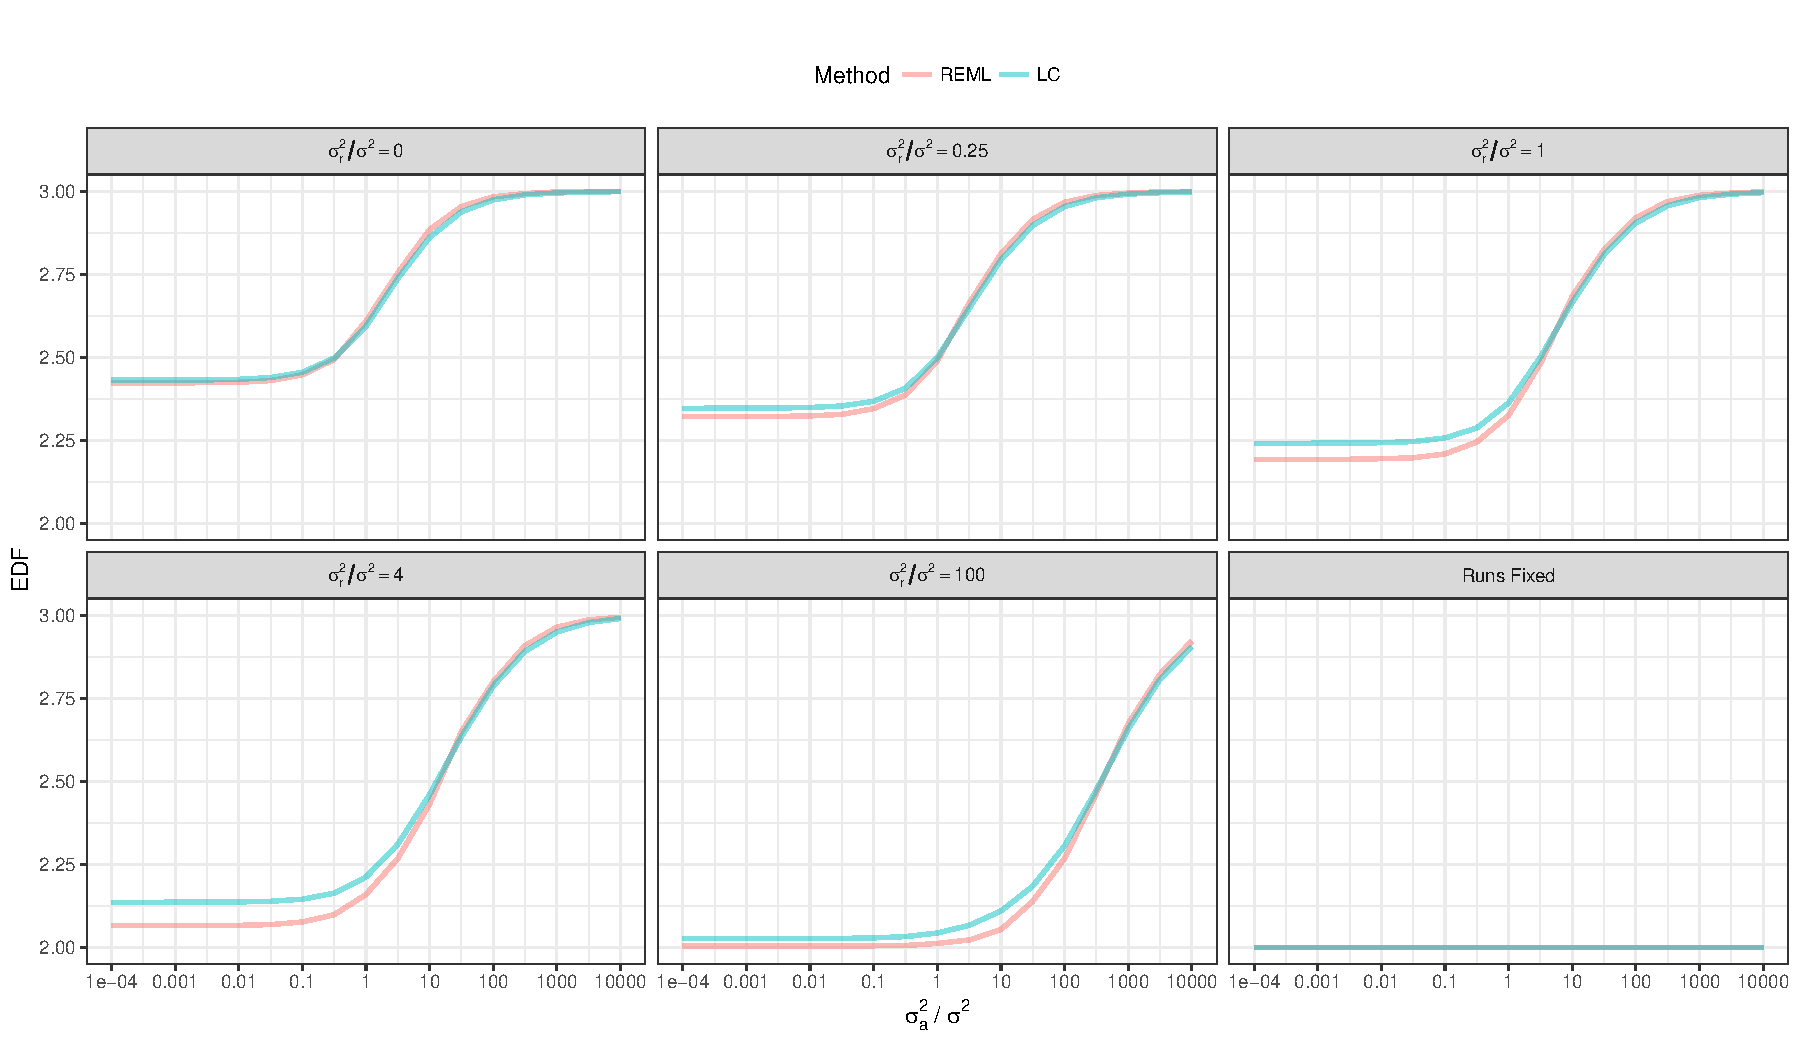
\includegraphics[width=1 \textwidth]{Chapter5/Graph/CRD232.pdf}
\caption{EDF for the variance of the treatment effects for two-phase experiment, i.e.\ for the optimal design of the Phase 2 experiment which takes account of the design of the Phase 1 experiment involves $\nu = 2$ treatments assigned to $n_a = 6$ animals. Each sample is further split into $n_s = 2$ sub-samples labelled by $n_\gamma = 4$ tags and measured in $n_r = 3$ runs, based on REML estimates of the variance components and on a linear combination of the mean squares.}
\label{fig:EDFadjusted}
\end{figure}

\section{EDF when Phase 1 experiment is arrange in a CRD}
\label{sec:expCRD}
This section compares the EDF obtained from optimal designs of the Phase 2 experiment found when the Phase 1 experiment is arranged in a CRD. The main consideration is on comparing four-plex and eight-plex experiments using an identical Phase 1 experiment. Three different cases are presented, showing that different sets of design parameters can work better depending on whether the four-plex or eight-plex experiment is used.

\subsection{Example 1: A CRD with 2 treatments and 12 animals}
The first example experiment to be considered is the Phase 1 experiment with $\nu = 2$ treatments assigned to $n_a = 12$ animals. Based on the methods presented in Chapter 3, two optimal designs are found for the Phase 2 proteomics experiment: one assuming the four-plex iTRAQ$^{\rm TM}$ system is used and the other assuming that the eight-plex system is used, which are presented in Tables~\ref{tab:aniDes1EDF} and \ref{tab:aniDes2EDF}, respectively.

\begin{table}[ht]
\centering   
\itshape 
\caption{Optimal (a) four- and (b) eight-plex designs of Phase 2 proteomics experiment when the Phase~1 experiment consists of $\nu = 2$ treatments assigned to each of $n_a = 12$ animals, with $n_s = 2$ sub-samples taken from each animal and analysed in the Phase 2 MudPIT-iTRAQ$^{\rm TM}$ experiment. Animal IDs are denoted by upper case letters, while the lower case letters a and b denote the two treatments.}
\begin{subtable}{.35 \linewidth} 
\caption{Four-plex system.}  
\begin{tabular}{c|cc:cc}
 & \multicolumn{4}{c}{{\bf Tag}} \\
{\bf Run}  & \textnormal{114} & \textnormal{115} & \textnormal{116} & \textnormal{117} \\ 
\hline  
\textnormal{1} & Jb & Aa & Lb & Ca \\ 
\textnormal{2} & Aa & Jb & Ca & Lb \\ 
\textnormal{3} & Ia & Fb & Hb & Ka \\ 
\textnormal{4} & Fb & Ia & Ka & Hb \\ 
\textnormal{5} & Bb & Ea & Db & Ga \\ 
\textnormal{6} & Ea & Bb & Ga & Db \\
\end{tabular} 
\label{tab:aniDes1EDF}
\end{subtable} 
\begin{subtable}{.5 \linewidth}   
\caption{Eight-plex system.}  
\begin{tabular}[t]{c|cc:cc:cc:cc}
 & \multicolumn{8}{c}{{\bf Tag}} \\
{\bf Run}  &  \textnormal{113} &  \textnormal{114} &  \textnormal{115} &  \textnormal{116} &  \textnormal{117} &  \textnormal{118} &  \textnormal{119} &  \textnormal{121}\\ \hline 
\textnormal{1} & Ia & Ea & Ga & Db & Hb & Ca & Bb & Jb \\ 
\textnormal{2} & Ea & Ia & Db & Ga & Ca & Hb & Jb & Bb \\ 
\textnormal{3} & Fb & Fb & Lb & Lb & Ka & Ka & Aa & Aa \\  
\end{tabular} 
\label{tab:aniDes2EDF}
\end{subtable}
\end{table}

The theoretical ANOVA tables for the four- and eight-plex optimal designs are presented in Tables~\ref{tab:ANOVAPhase1CRD11} and \ref{tab:ANOVAPhase1CRD12}, respectively. Based solely on these two theoretical ANOVA tables, the four-plex design is shown to be the better design, because it has higher Residual DF for estimating the Residual MS and therefore for testing treatment effects (7 DF compared to with 6 DF for the eight-plex design), and Treatment effects are fully estimated in the desired stratum, namely Between Animals within Runs. In comparison, the average efficiency factor for treatment effects in the eight-plex design is 0.889 due to the 1 DF of treatment contrast being partially confounded with the contrast of Tag 113, 114, 117, 118 versus Tag 115, 116, 119, 121. In addition, the theoretical ANOVA table of the four-plex experiment shows there are 2 DF associated with the residual variance in the Between Animals Between Runs stratum, potentially enabling the recovery of up to 2 additional DF, i.e.\ yielding up to 9 EDF. The eight-plex experiment has 1 DF associated with the Between Animals Between Runs stratum, which can be recovered giving EDF as high as 7 DF.  

\begin{table}[!ht]
\centering
 \caption{Theoretical ANOVA table for the optimal design of the Phase 2 experiment in Table~\ref{tab:aniDes1EDF}.}
 \begin{tabular}[t]{lrlll} 
 \toprule 
 \multicolumn{1}{l}{\textbf{Source of Variation}} & \multicolumn{1}{l}{\textbf{DF}} & \multicolumn{1}{l}{\textbf{EMS}}& \multicolumn{1}{l}{$\bm{E_{\gamma}}$}&\multicolumn{1}{l}{$\bm{E_{\tau}}$}\\ 
 \midrule 
 Between Runs &  &  & & \\ 
 \quad Between Animals & $2$ & $\sigma^2+2\sigma_{a}^2+4\sigma_{r}^2$ & & \\  \quad Within Animals & $3$ & $\sigma^2+4\sigma_{r}^2$ & & \\ \hline 
 Within Runs &  &  & & \\ 
 \quad Between Animals &  &  & & \\ 
 \quad \quad Tag & $1$ & $\sigma^2+2\sigma_{a}^2+6\theta_{\gamma}$ &$1$ & \\ 
 \quad \quad Treatment & $1$ & $\sigma^2+2\sigma_{a}^2+12\theta_{\tau}$ & & $1$\\ 
 \quad \quad Residual & $7$ & $\sigma^2+2\sigma_{a}^2$ & & \\ \hline 
 \quad Within Animals &  &  & & \\ 
 \quad \quad Tag & $2$ & $\sigma^2+6\theta_{\gamma}$ &$1$ & \\ 
 \quad \quad Residual & $7$ & $\sigma^2$ & & \\ 
 \bottomrule 
 \end{tabular} 
 \label{tab:ANOVAPhase1CRD11} 

\centering
 \caption{Theoretical ANOVA table for the optimal design of Phase 2 experiment in Table~\ref{tab:aniDes2EDF}.}
 \begin{tabular}[t]{lrlll} 
 \toprule 
 \multicolumn{1}{l}{\textbf{Source of Variation}} & \multicolumn{1}{l}{\textbf{DF}} & \multicolumn{1}{l}{\textbf{EMS}}& \multicolumn{1}{l}{$\bm{E_{\gamma}}$}&\multicolumn{1}{l}{$\bm{E_{\tau}}$}\\ 
 \midrule 
 Between Runs &  &  & & \\ 
 \quad Between Animals & $1$ & $\sigma^2+2\sigma_{a}^2+8\sigma_{r}^2$ & & \\  \quad Within Animals & $1$ & $\sigma^2+8\sigma_{r}^2$ & & \\ \hline 
 Within Runs &  &  & & \\ 
 \quad Between Animals &  &  & & \\ 
 \quad \quad Tag & $3$ & $\sigma^2+2\sigma_{a}^2+3\theta_{\gamma}+ 1.33\theta_{\tau}$ &$1$ & $0.1111$\\ 
 \quad \quad Treatment & $1$ & $\sigma^2+2\sigma_{a}^2+10.67\theta_{\tau}$ & & $0.8889$\\ 
 \quad \quad Residual & $6$ & $\sigma^2+2\sigma_{a}^2$ & & \\ \hline 
 \quad Within Animals &  &  & & \\ 
 \quad \quad Tag & $4$ & $\sigma^2+3\theta_{\gamma}$ &$1$ & \\ 
 \quad \quad Residual & $7$ & $\sigma^2$ & & \\ 
 \bottomrule 
 \end{tabular} 
 \label{tab:ANOVAPhase1CRD12} 
\end{table} 

\begin{figure}[!ht]
\centering
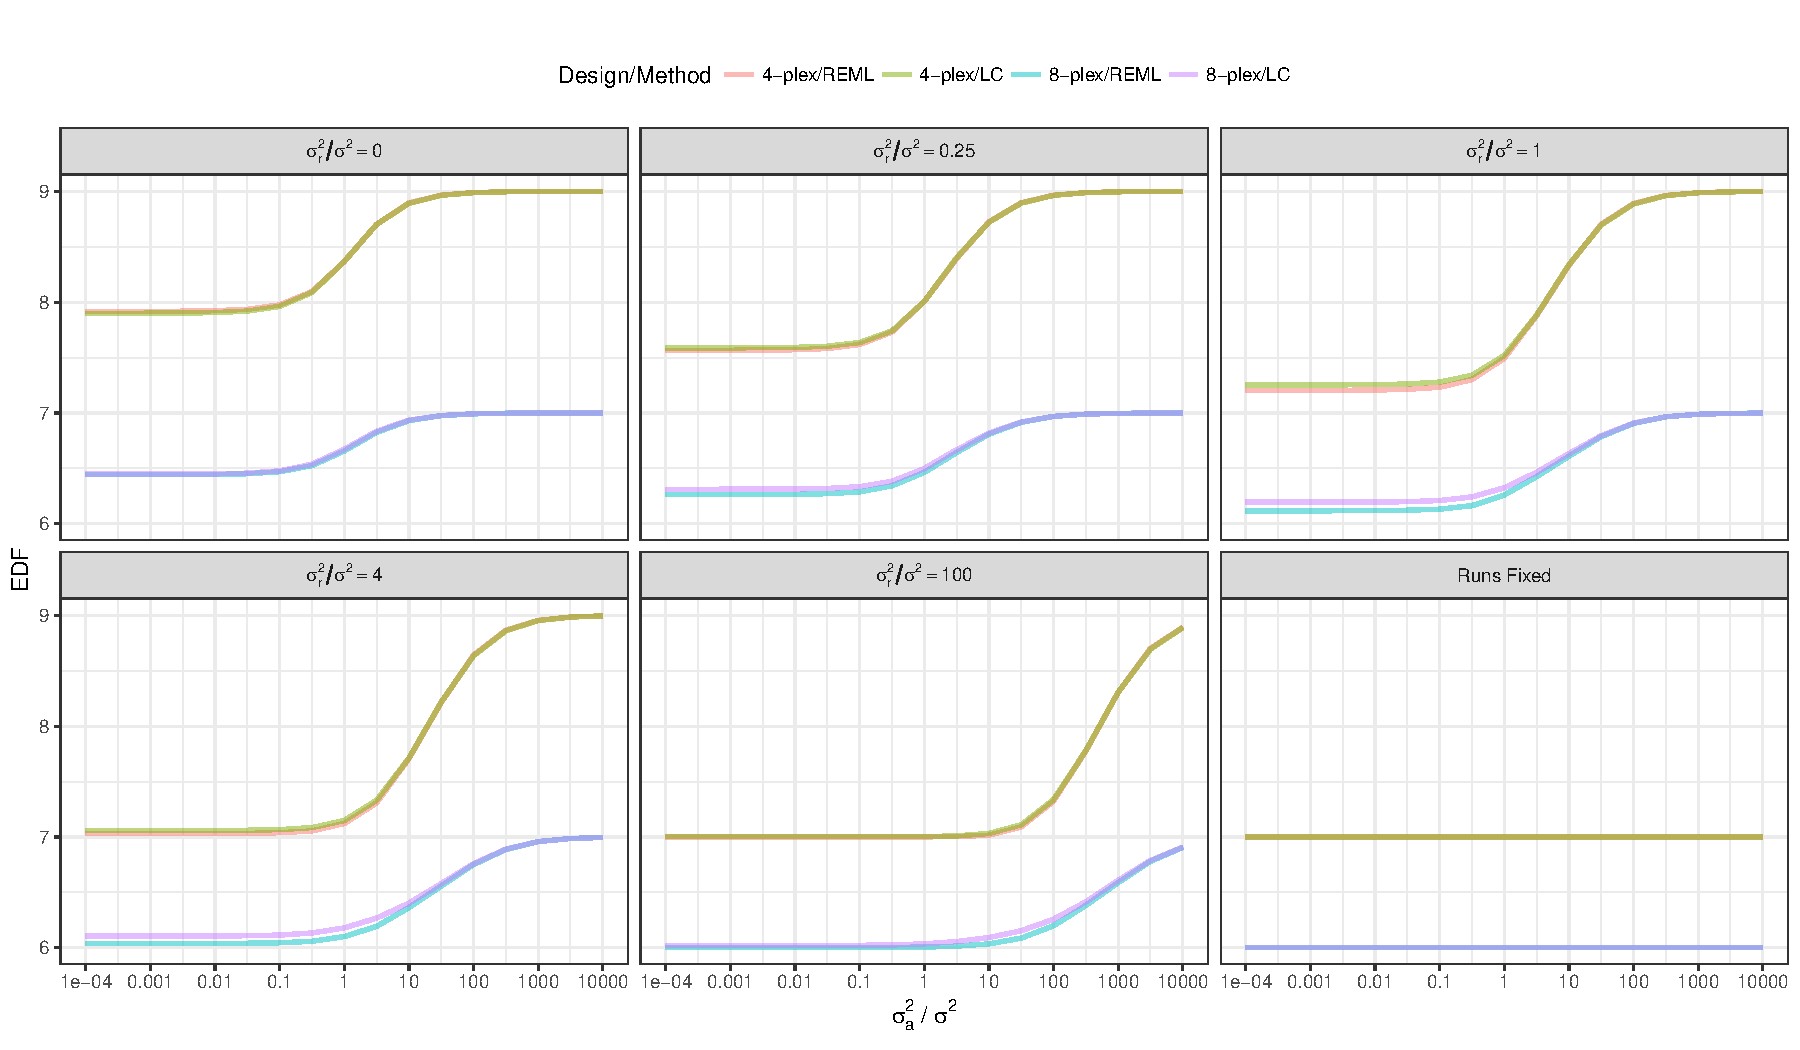
\includegraphics[width=1 \textwidth]{Chapter5/Graph/CRD262.pdf}
\caption{EDF plots for optimal designs shown in Tables~\ref{tab:aniDes1EDF} and \ref{tab:aniDes2EDF}, where EDF is calculated using VCs estimated by both the REML and LC methods.}
\label{fig:compare48CRD1}
\end{figure}

The EDF plots, in Figure~\ref{fig:compare48CRD1}, show that the EDF from the four-plex experiment is always higher than that from the  eight-plex experiment. The EDF of the four-plex experiment can be as low as 7 DF when there is large run-to-run variation, but the EDF approach 9 when the between-animal variation dominates. As for the eight-plex experiment, the EDF can be as low as 6 DF with large Run effects, but the EDF approach 7 with high between-animal variation. This suggests that the optimal design using the four-plex experiment is to be preferred over the eight-plex experiment in this case. In addition, the EDF appears to be very similar between the REML and LC methods.

\subsection{Example 2: A CRD with 8 treatments and 16 animals}
The second example experiment to be considered is a Phase 1 experiment with $\nu = 8$ treatments each assigned to $n_a = 16$ animals. Based on the methods presented in Chapter 3, two optimal designs are found for the Phase 2 proteomics experiment: one assuming the four-plex iTRAQ$^{\rm TM}$ system is used and the other assuming that the eight-plex system is used. These designs are presented in Tables~\ref{tab:aniDes3EDF} and \ref{tab:aniDes4EDF}, respectively.

\begin{table}[!ht]
\centering   
\itshape 
\caption{Optimal (a) four- and (b) eight-plex designs of Phase 2 proteomics experiment when the Phase~1 experiment consists of $\nu = 8$ treatments each assigned to $n_a = 16$ animals, with $n_s = 2$ sub-samples are then taken from each animal and analysed in the Phase 2 MudPIT-iTRAQ$^{\rm TM}$ experiment. Upper case letters denote animal IDs, while the lower case letters denote the treatments.}
\begin{subtable}{.35 \linewidth} 
\caption{Four-plex system.}  
\begin{tabular}{c|cc:cc}
 & \multicolumn{4}{c}{{\bf Tag}} \\
{\bf Run}  & \textnormal{114} & \textnormal{115} & \textnormal{116} & \textnormal{117} \\ 
\hline  
\textnormal{1} & Jb & Dd & Ph & Kc \\ 
\textnormal{2} & Dd & Jb & Kc & Ph \\ \hdashline
\textnormal{3} & Hh & Ee & Nf & Bb \\ 
\textnormal{4} & Ee & Hh & Bb & Nf \\ \hdashline
\textnormal{5} & Aa & Og & Me & Ld \\ 
\textnormal{6} & Og & Aa & Ld & Me \\ \hdashline
\textnormal{7} & Ff & Cc & Ia & Gg \\ 
\textnormal{8} & Cc & Ff & Gg & Ia \\ 
\end{tabular} 
\label{tab:aniDes3EDF}
\end{subtable} 
\begin{subtable}{.5 \linewidth}   
\caption{Eight-plex system.}  
\begin{tabular}[t]{c|cc:cc:cc:cc}
 & \multicolumn{8}{c}{{\bf Tag}} \\
{\bf Run}  &  \textnormal{113} &  \textnormal{114} &  \textnormal{115} &  \textnormal{116} &  \textnormal{117} &  \textnormal{118} &  \textnormal{119} &  \textnormal{121}\\ \hline 
\textnormal{1} & Ff & Dd & Kc & Hh & Me & Aa & Og & Bb \\ 
\textnormal{2} & Dd & Ff & Hh & Kc & Aa & Me & Bb & Og \\ \hdashline
\textnormal{3} & Cc & Ia & Nf & Jb & Gg & Ph & Ld & Ee \\ 
\textnormal{4} & Ia & Cc & Jb & Nf & Ph & Gg & Ee & Ld \\ 
\end{tabular} 
\label{tab:aniDes4EDF}
\end{subtable} 
\end{table}

The theoretical ANOVA tables for the four- and eight-plex optimal designs in Tables~\ref{tab:aniDes3EDF} and ~\ref{tab:aniDes4EDF} are presented in Tables~\ref{tab:ANOVAPhaseCRD31} and \ref{tab:ANOVAPhaseCRD32}, respectively. Based solely on these two theoretical ANOVA tables, both designs have the 4 Residual DF for estimating the Residual MS and therefore for testing Treatment effects. Furthermore, in both designs the Treatment effects are estimated, in the desired stratum, namely Between Animals within Runs, and have average efficiency factor \ $E_\tau = 0.8077$. 

For the four-plex experiment, the treatment average efficiency factor of $0.8077$ is due to the 3 DF associated with Treatment effects being confounded with Run effects. Thus, the Between Animals Between Runs EMS, which in previous cases provided a measure of pure error, now includes a contribution from the Treatment fixed effect. The 3 DF associated with this effect are not available for recovery of information, i.e. the existing 4 Residual DF for estimating the variance of the treatment effects cannot be improved upon. In comparison, although the treatment average efficiency factor, in the eight-plex design, is also $0.8077$, 3 of 7 DF associated with Treatment effects are now partially confounded with Tag effects. As a result, the 1 DF associated with the Between Animals MS in the Between Runs stratum remains pure error and can be recovered in the estimation of the VCs, resulting in the EDF to being as high as 5 DF. 


%thus, the mean square containing both the Between Animals VC, $\sigma_a^2$, and Between Runs VCs, $\sigma_r^2$, has to be regarded as fixed. Consequently, it is impossible to recover these 3 DF using the method presented in this Chapter. Therefore, the EDF for the four-plex experiment are always 4 DF.

\begin{table}[!ht]
\centering
 \caption{Theoretical ANOVA table for the optimal design of Phase 2 experiment in Table~\ref{tab:aniDes3EDF}.}
 \begin{tabular}[t]{lrlll} 
 \toprule 
 \multicolumn{1}{l}{\textbf{Source of Variation}} & \multicolumn{1}{l}{\textbf{DF}} & \multicolumn{1}{l}{\textbf{EMS}}& \multicolumn{1}{l}{$\bm{E_{\gamma}}$}&\multicolumn{1}{l}{$\bm{E_{\tau}}$}\\ 
 \midrule 
 Between Runs &  &  & & \\ 
 \quad Between Animals &  &  & & \\ 
 \quad \quad Treatment & $3$ & $\sigma^2+2\sigma_{a}^2+4\sigma_{r}^2+1.2\theta_{\tau}$ & & $0.3$\\ 
 \quad Within Animals & $4$ & $\sigma^2+4\sigma_{r}^2$ & & \\ \hline 
 Within Run &  &  & & \\ 
 \quad Between Animals &  &  & & \\ 
 \quad \quad Tag & $1$ & $\sigma^2+2\sigma_{a}^2+8\theta_{\gamma}$ &$1$ & \\ 
 \quad \quad Treatment & $7$ & $\sigma^2+2\sigma_{a}^2+ 3.23\theta_{\tau}$ & & $0.8077$\\ 
 \quad \quad Residual & $4$ & $\sigma^2+2\sigma_{a}^2$ & & \\ \hline 
 \quad Within Animals &  &  & & \\ 
 \quad \quad Tag & $2$ & $\sigma^2+8\theta_{\gamma}$ &$1$ & \\ 
 \quad \quad Residual & $10$ & $\sigma^2$ & & \\ 
 \bottomrule 
 \end{tabular} 
 \label{tab:ANOVAPhaseCRD31} 

 \caption{Theoretical ANOVA table for the optimal design of Phase 2 experiment in Table~\ref{tab:aniDes4EDF}.}
 \begin{tabular}[t]{lrlll} 
 \toprule 
 \multicolumn{1}{l}{\textbf{Source of Variation}} & \multicolumn{1}{l}{\textbf{DF}} & \multicolumn{1}{l}{\textbf{EMS}}& \multicolumn{1}{l}{$\bm{E_{\gamma}}$}&\multicolumn{1}{l}{$\bm{E_{\tau}}$}\\ 
 \midrule 
 Between Runs &  &  & & \\ 
 \quad Between Animals & $1$ & $\sigma^2+2\sigma_{a}^2+8\sigma_{r}^2$ & & \\ 
 \quad Within Animals & $2$ & $\sigma^2+8\sigma_{r}^2$ & & \\ \hline 
 Within Runs &  &  & & \\ 
 \quad Between Animals &  &  & & \\ 
 \quad \quad Tag & $3$ & $\sigma^2+2\sigma_{a}^2+4\theta_{\gamma}+1.2\theta_{\tau}$ &$1$ &  $0.3$\\ 
 \quad \quad Treatment & $7$ & $\sigma^2+2\sigma_{a}^2+3.23\theta_{\tau}$ & & $0.8077$\\ 
 \quad \quad Residual & $4$ & $\sigma^2+2\sigma_{a}^2$ & & \\ \hline 
 \quad Within Animals &  &  & & \\ 
 \quad \quad Tag & $4$ & $\sigma^2+4\theta_{\gamma}$ &$1$ & \\ 
 \quad \quad Residual & $10$ & $\sigma^2$ & & \\ 
 \bottomrule 
 \end{tabular} 
 \label{tab:ANOVAPhaseCRD32} 
\end{table} 

The EDF plots, in Figure~\ref{fig:compare82CRD}, show that the EDF for the design using the eight-plex system is always 4 irrespective of the values of the ratios $\sigma_a^2/\sigma^2$ and $\sigma_r^2/\sigma^2$. For the four-plex design, the EDF can be as low as 4 when the run-to-run variation is much larger than the between animal variation, and as high as 5 DF when the between-animal variation dominates. The EDF are the same (4 DF) between four- and eight-plex experiments when $\sigma_r^2/\sigma^2 = 100$ and $\sigma_a^2/\sigma^2$ is between $1 \times 10^{-4}$ to $10$, i.e.\ when the run-to-run  variation is 10 to $1 \times 10^{6}$ times of run-to-run variation over animal-to-animal variation. The EDF are also the same (4 DF) between four- and eight-plex experiments when Run effects are assumed to be fixed. In addition, the EDF are again shown to be very similar between the REML and LC methods.

\begin{figure}[!ht]
\centering
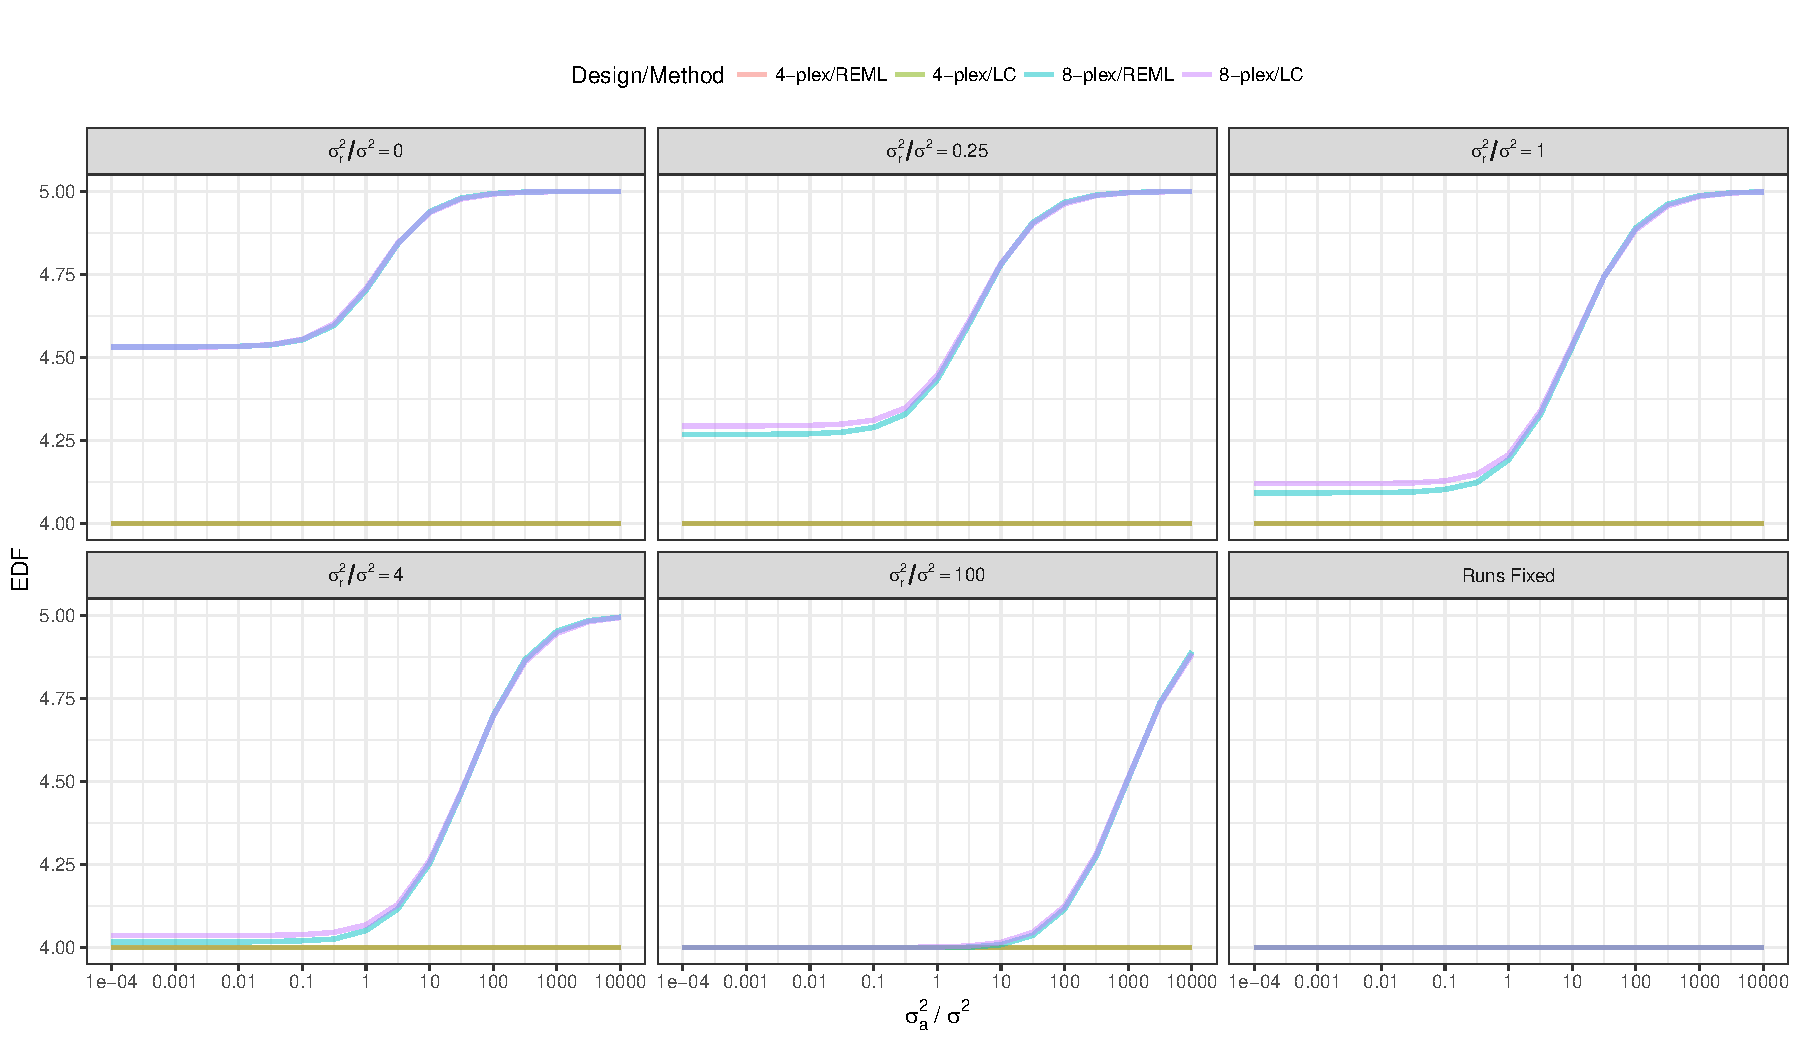
\includegraphics[width=1 \textwidth]{Chapter5/Graph/CRD822.pdf}
\caption{EDF plots for optimal designs shown in Tables~\ref{tab:aniDes3EDF} and \ref{tab:aniDes4EDF}, where EDF is calculated using VCs estimated by both the REML and LC methods.}
\label{fig:compare82CRD}
\end{figure}

\subsection{Example 3: A CRD with 4 treatments and 24 animals}
In the third example, the Phase 1 experiment involves $\nu = 4$ treatments assigned to $n_a = 24$ animals. Based on the methods presented in Chapter 3, two optimal designs are found for the Phase 2 proteomics experiment: one assuming the four-plex iTRAQ$^{\rm TM}$ system is used and the other assuming that the eight-plex system is used. These designs are presented in Tables~\ref{tab:aniDes5EDF} and \ref{tab:aniDes6EDF}, respectively.

\begin{table}[ht]
\centering
\itshape
\caption{Optimal (a) four- and (b) eight-plex designs of Phase 2 proteomics experiment, when the Phase~1 experiment consists of $\nu = 4$ treatments assigned to each of $n_a = 24$ animals, $n_s = 2$ sub-samples are then taken from each animal and analysed in the Phase 2 MudPIT-iTRAQ$^{\rm TM}$ experiment. Upper case letters denote animal IDs, while the lower case letters denote the treatments.}
\begin{subtable}{.35 \linewidth} 
\caption{Four-plex system.}  
\begin{tabular}{c|cc:cc}
 & \multicolumn{4}{c}{{\bf Tag}} \\
{\bf Run}  & \textnormal{114} & \textnormal{115} & \textnormal{116} & \textnormal{117} \\ 
\hline  
\textnormal{1} & Aa & Rb & Cc & Dd \\ 
\textnormal{2}  2 & Rb & Aa & Dd & Cc \\ \hdashline
\textnormal{3}  3 & Ea & Fb & Gc & Hd \\ 
\textnormal{4}  4 & Fb & Ea & Hd & Gc \\ \hdashline
\textnormal{5}  5 & Ia & Jb & Kc & Ld \\ 
\textnormal{6}  6 & Jb & Ia & Ld & Kc \\ \hdashline
\textnormal{7}  7 & Oc & Pd & Ma & Nb \\ 
\textnormal{8}  8 & Pd & Oc & Nb & Ma \\ \hdashline
\textnormal{9}  9 & Sc & Td & Qa & Bb \\ 
\textnormal{10}  10 & Td & Sc & Bb & Qa \\ \hdashline
\textnormal{11}  11 & Wc & Xd & Ua & Vb \\ 
\textnormal{12}  12 & Xd & Wc & Vb & Ua \\ 
\end{tabular} 
\label{tab:aniDes5EDF}
\end{subtable} 
\begin{subtable}{.5 \linewidth}   
\caption{Eight-plex system.} 
\begin{tabular}[t]{c|cc:cc:cc:cc}
 & \multicolumn{8}{c}{{\bf Tag}} \\
{\bf Run}  &  \textnormal{113} &  \textnormal{114} &  \textnormal{115} &  \textnormal{116} &  \textnormal{117} &  \textnormal{118} &  \textnormal{119} &  \textnormal{121}\\ \hline 
\textnormal{1} & Vb & Ma & Qa & Pd & Dd & Wc & Bb & Oc \\ 
\textnormal{2} & Ma & Vb & Pd & Qa & Wc & Dd & Oc & Bb \\ \hdashline
\textnormal{3} & Kc & Rb & Td & Cc & Jb & Ea & Aa & Hd \\ 
\textnormal{4} & Rb & Kc & Cc & Td & Ea & Jb & Hd & Aa \\ \hdashline
\textnormal{5} & Sc & Ld & Fb & Nb & Xd & Ua & Gc & Ia \\ 
\textnormal{6} & Ld & Sc & Nb & Fb & Ua & Xd & Ia & Gc \\ 
\end{tabular} 
\label{tab:aniDes6EDF}
\end{subtable} 
\end{table}

The theoretical ANOVA tables for the four- and eight-plex optimal designs in Tables~\ref{tab:aniDes5EDF} and \ref{tab:aniDes6EDF} are presented in Tables~\ref{tab:ANOVAPhase1CRD21} and \ref{tab:ANOVAPhase1CRD22}, respectively. Based solely on these two theoretical ANOVA tables, the eight-plex design  has higher Residual DF for estimating the Residual MS and for testing treatment effects (15 DF compared 14 DF for the four-plex design). Comparing the treatment average efficiency factor from the two designs: $E_\tau = 0.9623$ for the eight-plex design which is slightly lower than $E_\tau =1$ for the four-plex design. In addition, the theoretical ANOVA table of the four-plex design has 5 DF associated with the Between Animals Between Runs stratum, which can be recovered giving EDF as high as 19, whereas the eight-plex experiment has 2 DF associated with the Between Animals Between Runs stratum, which can be recovered giving EDF as high as 17.  

\begin{table}[!ht]
\centering
 \caption{Theoretical ANOVA table for the optimal design of Phase 2 experiment in Table~\ref{tab:aniDes5EDF}.}
 \begin{tabular}[t]{lrlll} 
 \toprule 
 \multicolumn{1}{l}{\textbf{Source of Variation}} & \multicolumn{1}{l}{\textbf{DF}} & \multicolumn{1}{l}{\textbf{EMS}}& \multicolumn{1}{l}{$\bm{E_{\gamma}}$}&\multicolumn{1}{l}{$\bm{E_{\tau}}$}\\ 
 \midrule 
 Between Runs &  &  & & \\ 
 \quad Between Animals & $5$ & $\sigma^2+2\sigma_{a}^2+4\sigma_{r}^2$ & & \\  \quad Within Animals & $6$ & $\sigma^2+4\sigma_{r}^2$ & & \\ \hline 
 Within Runs &  &  & & \\ 
 \quad Between Animals &  &  & & \\ 
 \quad \quad Tag & $1$ & $\sigma^2+2\sigma_{a}^2+12\theta_{\gamma}$ &$1$ & \\ 
 \quad \quad Treatment & $3$ & $\sigma^2+2\sigma_{a}^2+12\theta_{\tau}$ & & $1$\\ 
 \quad \quad Residual & $14$ & $\sigma^2+2\sigma_{a}^2$ & & \\ \hline 
 \quad Within Animals &  &  & & \\ 
 \quad \quad Tag & $2$ & $\sigma^2+12\theta_{\gamma}$ &$1$ & \\ 
 \quad \quad Residual & $16$ & $\sigma^2$ & & \\ 
 \bottomrule 
 \end{tabular} 
 \label{tab:ANOVAPhase1CRD21} 

 \caption{Theoretical ANOVA table for the optimal design of Phase 2 experiment in Table~\ref{tab:aniDes6EDF}.}
 \begin{tabular}[t]{lrlll} 
 \toprule 
 \multicolumn{1}{l}{\textbf{Source of Variation}} & \multicolumn{1}{l}{\textbf{DF}} & \multicolumn{1}{l}{\textbf{EMS}}& \multicolumn{1}{l}{$\bm{E_{\gamma}}$}&\multicolumn{1}{l}{$\bm{E_{\tau}}$}\\ 
 \midrule 
 Between Runs &  &  & & \\ 
 \quad Between Animals & $2$ & $\sigma^2+2\sigma_{a}^2+8\sigma_{r}^2$ & & \\  \quad Within Animals & $3$ & $\sigma^2+8\sigma_{r}^2$ & & \\ \hline 
 Within Runs &  &  & & \\ 
 \quad Between Animals &  &  & & \\ 
 \quad \quad Tag & $3$ & $\sigma^2+2\sigma_{a}^2+6\theta_{\gamma}+ 0.67\theta_{\tau}$ &$1$ & $0.0556$\\ 
 \quad \quad Treatment & $3$ & $\sigma^2+2\sigma_{a}^2+11.55\theta_{\tau}$ & & $0.9623$\\ 
 \quad \quad Residual & $15$ & $\sigma^2+2\sigma_{a}^2$ & & \\ \hline 
 \quad Within Animals &  &  & & \\ 
 \quad \quad Tag & $4$ & $\sigma^2+6\theta_{\gamma}$ &$1$ & \\ 
 \quad \quad Residual & $17$ & $\sigma^2$ & & \\ 
 \bottomrule 
 \end{tabular} 
 \label{tab:ANOVAPhase1CRD22} 
\end{table} 

\begin{figure}[!h]
\centering
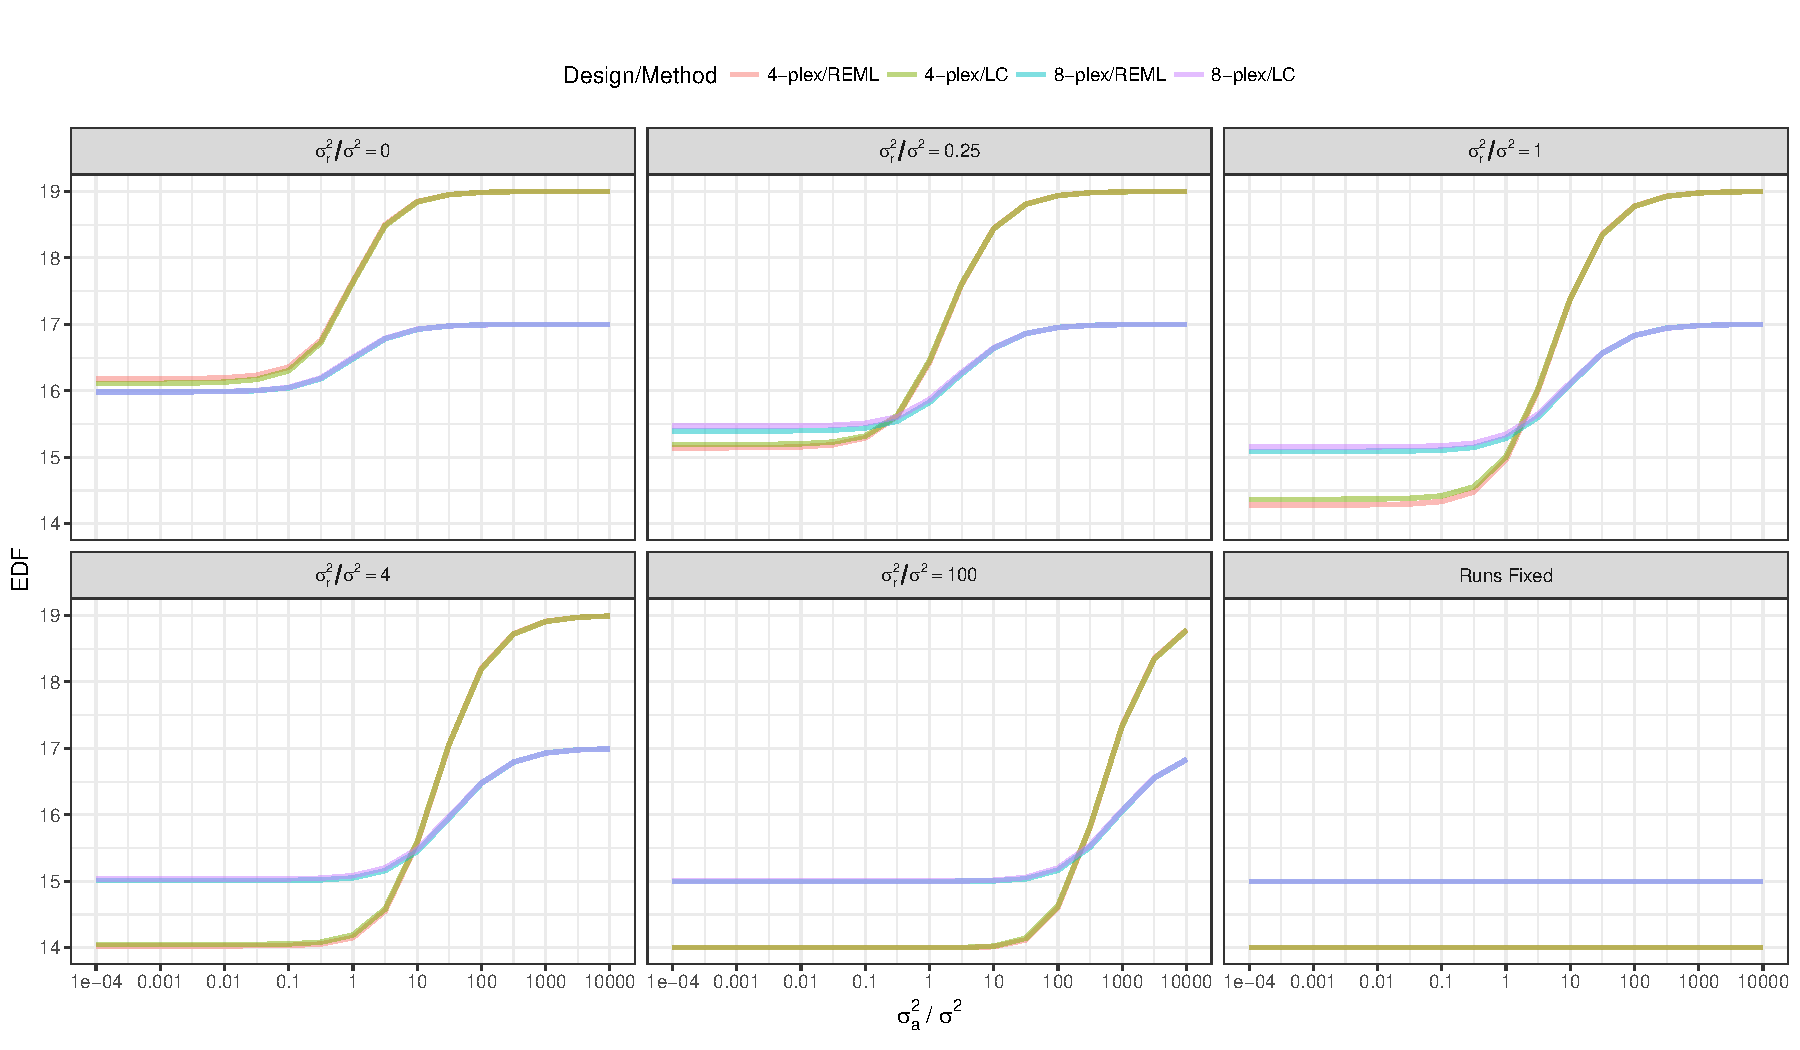
\includegraphics[width=1 \textwidth]{Chapter5/Graph/CRD462.pdf}
\caption{EDF plots for optimal designs shown in Tables~\ref{tab:aniDes5EDF} and \ref{tab:aniDes6EDF}, where EDF is calculated using VCs estimated by both the REML and LC methods.}
\label{fig:compare44CRD}
\end{figure}

The EDF plots, in Figure~\ref{fig:compare44CRD}, show that, for the design using the four-plex experiment, the EDF can be as low as 14 when the run-to-run variation is much larger than the between-animal variation, and as high as 19 when between-animal variation dominates. For the the design using eight-plex experiment, the EDF can be as low as 15 DF when the run-to-run variation is much larger than the between-animal variation, and as high as 17 DF when the between-animal variation dominates. Furthermore, recall from the theoretical ANOVA tables (in Tables~\ref{tab:ANOVAPhase1CRD21} and \ref{tab:ANOVAPhase1CRD22}) that the eight-plex design has 15 Residual DF compared with 14 Residual DF in the four-plex design. From the EDF plots, we can see the EDF for the four-plex design exceed those of the eight-plex design as $\sigma_a^2/\sigma^2$ increases. For example, when $\sigma_r^2/\sigma^2 = 0.25$, the EDF become higher for the four-plex experiment when $\sigma_a^2/\sigma^2 = 1 \times 10^{-0.5}$, that is about $0.79$ times of the run-to-run variation over animal-to-animal variation. Table~\ref{tab:edfCompare} lists the $\sigma_r^2/\sigma^2$ and $\sigma_a^2/\sigma^2$ combinations when the EDF become higher for the four-plex experiment than the eight-plex experiment, and the magnitudes of the run-to-run variation over animal-to-animal variation based on Figure~\ref{fig:compare44CRD}. 

\begin{table}[!h]
\centering
\caption{Magnitudes of the run-to-run variation over animal-to-animal variation when the EDF become higher for four-plex experiment than eight-plex experiments based on Figure~\ref{fig:compare44CRD}.}
\begin{tabular}{|c|l|l|l|l|}
\hline 
$\sigma_r^2/\sigma^2$ 	& $0.25$ & $1$ & $4$ & $100$ \\ 
\hline 
$\sigma_a^2/\sigma^2$ 	& $10^{-0.5}$ & $10^{0.25}$ & $10$ & $10^{2.25}$ \\ 
\hline 
$\sigma_r^2/\sigma_a^2$ 	 & $0.79$ & $0.56$ & $0.4$ & $0.32$ \\ 
\hline 
\end{tabular} 
\label{tab:edfCompare}
\end{table}

% When $\sigma_r^2/\sigma^2 = 1$, the EDF become higher for four-plex experiment when $\sigma_a^2/\sigma^2 = 1 \times 10^{0.25}$, that is about $0.56$ times of the run-to-run variation over animal-to-animal variation. When $\sigma_r^2/\sigma^2 = 4$, the EDF become higher for four-plex experiment when $\sigma_a^2/\sigma^2 = 10$, that is about $0.4$ times of the run-to-run variation over animal-to-animal variation. Finally, when $\sigma_r^2/\sigma^2 = 100$, the EDF become higher for four-plex experiment when $\sigma_a^2/\sigma^2 = 1 \times 10^{2.25}$, that is about $0.32$ times of the run-to-run variation over animals to animal variation. In addition, the EDF again shown to be not different between the REML and LC methods.


\section{Comparing the EDF when Phase 1 experiment is arranged in a RCBD}
\label{sec:expRCBD}
This section compares the EDF of optimal designs between Phase 2 four-plex and eight-plex experiments when the Phase 1 experiment is arranged in a RCBD. There are four types of designs that can be compared, given the same Phase 1 experiment is arranged in a RCBD: 
\begin{enumerate}
\item Phase 1 Block effects are intentionally confounded with Run effects using the four-plex system,
\item Phase 1 Block effects are intentionally confounded with Tag effects using the four-plex system,
\item Phase 1 Block effects are intentionally confounded with Run effects using the eight-plex system and
\item Phase 1 Block effects are intentionally confounded with Tag effects using the eight-plex system,
\end{enumerate}
The same method for estimating the VCs and approximating the EDF can also be applied to this example, because we can still construct an ANOVA table with Residual MS which assumed to have a chi-square distribution. In addition, the EDF are still approximated based on the Residual MS of the Between Experimental units (Plants) Within Blocks (Trays) Within Runs stratum, i.e.\ $\sigma^2 + \sigma_p^2$.

This section first compares designs from two different confounding schemes for each four- and eight-plex experiment, followed by an overall comparison between the four- and eight-plex systems. The Phase 2 experiment uses plants as an example when the Phase 1 experiment involves $\nu = 4$ treatments assigned to $n_p = 16$ plants in $n_b = 4$ trays. Then $n_s = 2$ sub-samples are obtained from each plant, i.e.\ a total of 32 sub-samples, for the Phase 2 proteomics experiment.  

The simulation study was done on the basis that MS has at chi-square distribution, with the ratio of Between Plants VCs to measurement error, denoted by $\sigma_p^2/\sigma^2$, set with 17 values ranging from $10^{-4}$ to $10^4$, the ratio of Between Trays VCs to measurement error and Between Runs VCs to measurement error, denoted by $\sigma_b^2/\sigma^2$ and $\sigma_r^2/\sigma^2$, respectively, set to $0, 0.25, 1, 5, 100$, as well as having effects of tray and run fixed are also considered (effectively when $\sigma _b^2 = \infty$ and $\sigma _r^2 = \infty$). 

\subsection{Four-plex system}
Given the Phase 1 experiment with $\nu = 4$ treatments assigned to $n_a = 16$ plants in $n_b = 4$ trays, based on the methods presented in Chapter 4, two optimal designs are found for the Phase 2 four-plex proteomics experiment: one assumes that Tray effects are intentionally confounded with Run effects, and the other that Tray effects are intentionally confounded with Tag effects. These are presented in Tables~\ref{tab:aniDes5EDF} and \ref{tab:aniDes6EDF}, respectively.

\begin{table}[!ht]
\centering   
\itshape 
\caption{Optimal design of Phase 2 proteomics experiment showing allocation of sub-samples from trays, plants and treatments to runs and tags, when the Phase~1 experiment consists of $\nu = 2$ treatments assigned to $n_a = 16$ plants in $n_b = 4$ trays, $n_s = 2$ sub-samples are then taken from each plant and analysed in the Phase 2 MudPIT-iTRAQ$^{\rm TM}$ experiment using $n_\gamma = 4$ tags. Numbers denote trays, upper case letters denote plant IDs, while the lower case letters denote the treatments.}
\begin{subtable}{.35 \linewidth} 
\caption{Tray effects are intentionally confounded with Run effects.}  
\begin{tabular}{c|cc:cc}
 & \multicolumn{4}{c}{{\bf Tag}} \\
{\bf Run}  & \textnormal{114} & \textnormal{115} & \textnormal{116} & \textnormal{117} \\ 
\hline  
\textnormal{1} & 1Cc & 1Dd & 1Bb & 1Aa \\ 
\textnormal{2} & 1Dd & 1Cc & 1Aa & 1Bb \\ \hdashline
\textnormal{3} & 2Hd & 2Fb & 2Ea & 2Gc \\ 
\textnormal{4} & 2Fb & 2Hd & 2Gc & 2Ea \\ \hdashline
\textnormal{5} & 3Ia & 3Jb & 3Ld & 3Kc \\ 
\textnormal{6} & 3Jb & 3Ia & 3Kc & 3Ld \\ \hdashline
\textnormal{7} & 4Ma & 4Oc & 4Pd & 4Nb \\ 
\textnormal{8} & 4Oc & 4Ma & 4Nb & 4Pd \\ 
\end{tabular} 
\label{tab:aniTrayDes1EDF}
\end{subtable} 
\begin{subtable}{.35 \linewidth}   
\caption{Tray effects are intentionally confounded with Tag effects.}  
\begin{tabular}{c|cc:cc}
 & \multicolumn{4}{c}{{\bf Tag}} \\
{\bf Run}  & \textnormal{114} & \textnormal{115} & \textnormal{116} & \textnormal{117} \\ 
\hline  
\textnormal{1} & 1Bb & 1Dd & 3Kc & 3Ia \\ 
\textnormal{2} & 1Dd & 1Bb & 3Ia & 3Kc \\ 
\textnormal{3} & 1Cc & 1Aa & 3Ld & 3Jb \\ 
\textnormal{4} & 1Aa & 1Cc & 3Jb & 3Ld \\ \hdashline
\textnormal{5} & 2Gc & 2Fb & 4Ma & 4Pd \\ 
\textnormal{6} & 2Fb & 2Gc & 4Pd & 4Ma \\ 
\textnormal{7} & 2Ea & 2Hd & 4Nb & 4Oc \\ 
\textnormal{8} & 2Hd & 2Ea & 4Oc & 4Nb \\ 
\end{tabular} 
\label{tab:aniTrayDes2EDF}
\end{subtable} 
\end{table}

The theoretical ANOVA tables for the optimal designs of the Phase 2 experiment using the four-plex system are presented in Tables~\ref{tab:ANOVAPhase1RCBD1} and \ref{tab:ANOVAPhase1RCBD2}, respectively. Based solely on these two theoretical ANOVA tables, the design when Tray effects are intentionally confounded with Run effects is shown to be the better design, because it has higher Residual DF for estimating the Residual MS and therefore for testing Treatment effects (8 DF compared to 7 DF for the four-plex design) in the Between Plants Within Trays stratum. Both designs can estimate Treatment effects with full efficiency in the Between Plants Within Trays stratum, because the treatment average efficiency factors for both designs are 100\%. 

From the theoretical ANOVA of both designs, there is extra information on the Between Plants VC $\sigma_{p}^2$ in the Between Trays Between Runs MS, however, we may not be able to recover this information, because we cannot equate Residual MS in Between Trays Between Runs stratum based on the EMS to estimate $\sigma_{p}^2$. For the design when the Tray effects are intentionally confounded the Run effects (see Table~\ref{tab:ANOVAPhase1RCBD2}), there are 2 DF associated with the Between Plants Within Blocks Between Runs stratum which can be recovered giving EDF as high as 9.  

\begin{table}[!ht]
\centering
 \caption{Theoretical ANOVA table from the Phase 2 experiment in Table~\ref{tab:aniTrayDes1EDF}.}
 \begin{tabular}[t]{lrlll} 
 \toprule 
 \multicolumn{1}{l}{\textbf{Source of Variation}} & \multicolumn{1}{l}{\textbf{DF}} & \multicolumn{1}{l}{\textbf{EMS}}& \multicolumn{1}{l}{$\bm{E_{\gamma}}$}&\multicolumn{1}{l}{$\bm{E_{\tau}}$}\\ 
 \midrule 
 Between Runs &  &  & & \\ 
 \quad Between Trays & $3$ & $\sigma^2+2\sigma_{p}^2+8\sigma_{b}^2+4\sigma_{r}^2$ & & \\  
 \quad Within Plants Within Trays & $4$ & $\sigma^2+4\sigma_{r}^2$ & & \\ \hline 
 Within Runs &  &  & & \\ 
 \quad Between Plants Within Trays &  &  & & \\ 
 \quad \quad Tag & $1$ & $\sigma^2+2\sigma_{p}^2+8\theta_{\gamma}$ &$1$ & \\ 
 \quad \quad Treatment & $3$ & $\sigma^2+2\sigma_{p}^2+8\theta_{\tau}$ & & $1$\\ 
 \quad \quad Residual & $8$ & $\sigma^2+2\sigma_{p}^2$ & & \\ \hline 
 \quad Within Plants Within Trays &  &  & & \\ 
 \quad \quad Tag & $2$ & $\sigma^2+8\theta_{\gamma}$ &$1$ & \\ 
 \quad \quad Residual & $10$ & $\sigma^2$ & & \\ 
 \bottomrule 
 \end{tabular} 
 \label{tab:ANOVAPhase1RCBD1} 

 \caption{Theoretical ANOVA table from the Phase 2 experiment in Table~\ref{tab:aniTrayDes2EDF}.}
 \begin{tabular}[t]{lrlll} 
 \toprule 
 \multicolumn{1}{l}{\textbf{Source of Variation}} & \multicolumn{1}{l}{\textbf{DF}} & \multicolumn{1}{l}{\textbf{EMS}}& \multicolumn{1}{l}{$\bm{E_{\gamma}}$}&\multicolumn{1}{l}{$\bm{E_{\tau}}$}\\ 
 \midrule 
 Between Runs &  &  & & \\ 
 \quad Between Trays & $1$ & $\sigma^2+2\sigma_{p}^2+8\sigma_{b}^2+4\sigma_{r}^2$ & & \\  
 \quad Between Plants Within Trays & $2$ & $\sigma^2+2\sigma_{p}^2+4\sigma_{r}^2$ & & \\  
 \quad Within Plants Within Trays & $4$ & $\sigma^2+4\sigma_{r}^2$ & & \\ \hline 
 Within Runs &  &  & & \\ 
 \quad Between Trays &  &  & & \\ 
 \quad \quad Tag & $1$ & $\sigma^2+2\sigma_{p}^2+8\sigma_{b}^2+8\theta_{\gamma}$ &$1$ & \\ 
 \quad \quad Residual & $1$ & $\sigma^2+2\sigma_{p}^2+8\sigma_{b}^2$ & & \\ \hline 
 \quad Between Plants Within Trays &  &  & & \\ 
 \quad \quad Treatment & $3$ & $\sigma^2+2\sigma_{p}^2+8\theta_{\tau}$ & & $1$\\ 
 \quad \quad Residual & $7$ & $\sigma^2+2\sigma_{p}^2$ & & \\ \hline 
 \quad Within Plants Within Trays &  &  & & \\ 
 \quad \quad Tag & $2$ & $\sigma^2+8\theta_{\gamma}$ &$1$ & \\ 
 \quad \quad Residual & $10$ & $\sigma^2$ & & \\ 
 \bottomrule 
 \end{tabular} 
 \label{tab:ANOVAPhase1RCBD2} 
\end{table} 

\begin{landscape}
\begin{figure}[h!]
\centering
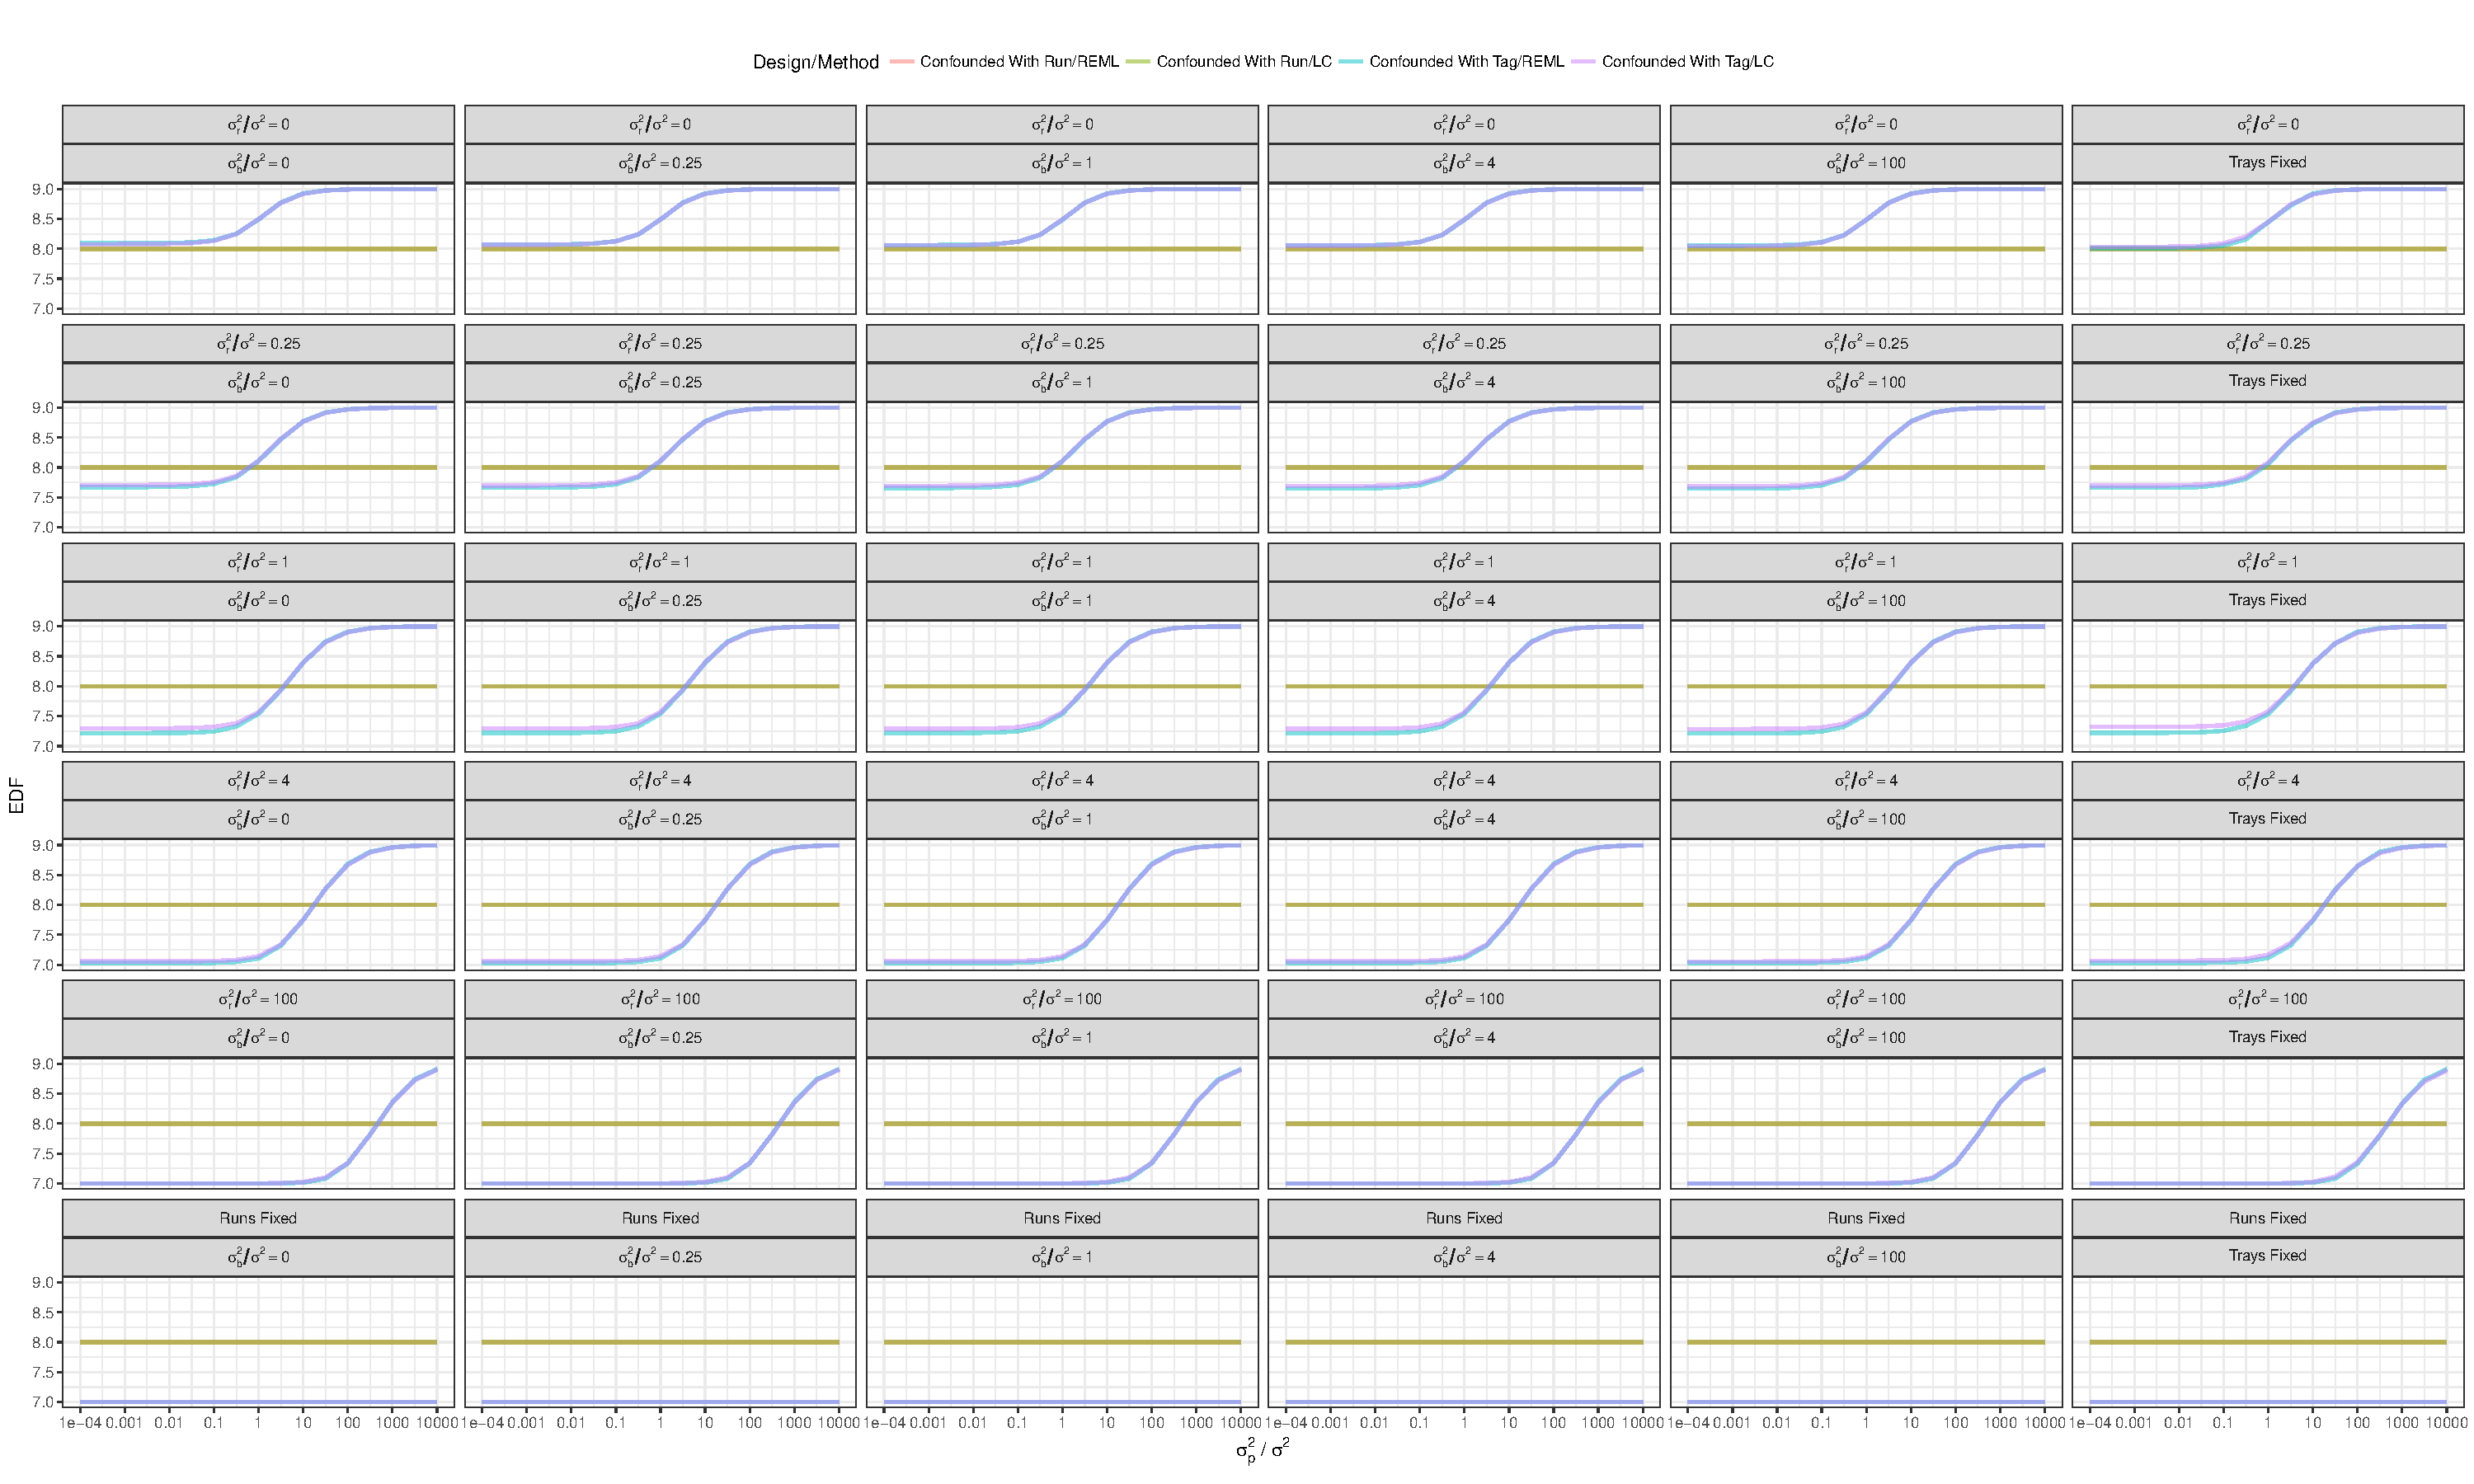
\includegraphics[width=1.3 \textwidth]{Chapter5/Graph/CRD44424.pdf}
\caption{EDF plots for optimal designs shown in Tables~\ref{tab:aniTrayDes1EDF} and \ref{tab:aniTrayDes2EDF}, where EDF is calculated using VCs estimated by both the REML and LC methods.}
\label{fig:RCBD442Tag4EDF}
\end{figure}
\end{landscape}

The EDF plots in Figure~\ref{fig:RCBD442Tag4EDF} are presented as a 6-by-6 panels having different combination of ranges of ratios for Between Plants VCs, Between Trays VCs and Between Runs VCs to measurement error, denoted by $\sigma_p^2/\sigma^2$, $\sigma_b^2/\sigma^2$ and $\sigma_r^2/\sigma^2$, respectively. We can first observe that different values of the ratio $\sigma_b^2/\sigma^2$ do not change the EDF. For the design when Tray effects are intentionally confounded with Run effects, the EDF are always 8 DF. For the design when Tray effects are intentionally confounded with Tag effects, the EDF can be as low as 7 DF when run-to-run variation is much larger than the between-plants variation, but the EDF approach 9 DF when the between-plants variation dominates. From the EDF plot, we can see that the EDF of the design when Tray effects are intentionally confounded with Tag effects become better than the design when Tray effects are intentionally confounded with Run effects as $\sigma_p^2/\sigma^2$ increases. For example, when $\sigma_r^2/\sigma^2 = 0.25$, the EDF become higher when $\sigma_p^2/\sigma^2 = 1$, that is about $0.25$ times of the run-to-run variation over plant-to-plant variation. Table~\ref{tab:edfCompare} lists the $\sigma_r^2/\sigma^2$ and $\sigma_p^2/\sigma^2$ combinations when the EDF become higher for the design when Tray effects are intentionally confounded with Tag effects than the design when Tray effects are intentionally confounded with Run effects, and the magnitudes of the run-to-run variation over plant-to-plant variation are based on Figure~\ref{fig:compare44CRD}. In addition, the EDF are again shown to be very similar between the REML and LC methods.

\begin{table}[!h]
\centering
\caption{Magnitudes of the run-to-run variation over plant-to-plant variation when the EDF become higher for design when Tray effects are intentionally confounded with Tag effects than the design when Tray effects are intentionally confounded with Run effect based on Figure~\ref{fig:RCBD442Tag4EDF}.}
\begin{tabular}{|c|l|l|l|l|}
\hline 
$\sigma_r^2/\sigma^2$ 	& $0.25$ & $1$ & $4$ & $100$ \\ 
\hline 
$\sigma_p^2/\sigma^2$ 	& $1$ & $ 10^{0.5}$ & $10^{1.25}$ & $10^{2.75}$ \\ 
\hline 
$\sigma_r^2/\sigma_p^2$ & $0.25$ & $0.32$ & $0.22$ & $0.18$ \\ 
\hline 
\end{tabular} 
\label{tab:edfCompare1}
\end{table}


%The example experiment to be considered features a Phase 1 experiment consisting of $\nu = 4$, $r_b = 4, n_B  = 4$ and $r_t = 2$. Four different two-phase designs can be compared using the same Phase 1 experiment. The theoretical ANOVA tables for each of these four designs are presented in Tables~\ref{tab:ANOVAPhase1RCBD1}, \ref{tab:ANOVAPhase1RCBD2}, \ref{tab:ANOVAPhase1RCBD3} and \ref{tab:ANOVAPhase1RCBD4}. Based on these four theoretical ANOVA tables, Tables~\ref{tab:ANOVAPhase1RCBD1} and \ref{tab:ANOVAPhase1RCBD4} appear to perform equally well, with the most residual DF of 8 and $100\%$ of the treatment information in the Between Plants Within Trays Within Runs stratum. The EDF are then assessed for each of these four designs. 


\subsection{Eight-plex system}
Using the same Phase 1 experiment with $\nu = 4$ treatments assigned to $n_a = 16$ plants in $n_b = 4$ trays, there are two optimal design that are found in the Phase 2 proteomics experiment using the eight-plex system. The first design assumes that the Tray effects are intentionally confounded with Run effects (see Tables~\ref{tab:aniDes5EDF}). The second design assumes that Tray effects are intentionally confounded with Tag effects (see Tables~\ref{tab:aniDes5EDF}).

\begin{table}[!ht]
\centering   
\itshape 
\caption{Optimal design of Phase 2 proteomics experiment showing allocation of sub-samples from trays, plants and treatments to runs and tags, when the Phase~1 experiment consists of $\nu = 2$ treatments assigned to $n_a = 16$ plants in $n_b = 4$ trays, $n_s = 2$ sub-samples are then taken from each plant and analysed in the Phase 2 MudPIT-iTRAQ$^{\rm TM}$ experiment using $n_\gamma = 8$ tags. Numbers denote trays, upper case letters denote plant IDs, while the lower case letters denote the treatments.}
\begin{subtable}{.55 \linewidth} 
\caption{Tray effects are intentionally confounded with Run effects.}  
\begin{tabular}[t]{c|cccc:cccc}
 & \multicolumn{8}{c}{{\bf Tag}} \\
{\bf Run}  &  \textnormal{113} &  \textnormal{114} &  \textnormal{115} &  \textnormal{116} &  \textnormal{117} &  \textnormal{118} &  \textnormal{119} &  \textnormal{121}\\ \hline 
\textnormal{1} & 1Bb & 1Dd & 1Aa & 1Cc & 2Ea & 2Fb & 2Gc & 2Hd \\ 
\textnormal{2} & 1Dd & 1Bb & 1Cc & 1Aa & 2Fb & 2Ea & 2Hd & 2Gc \\ \hdashline
\textnormal{3} & 3Ia & 3Kc & 3Ld & 3Jb & 4Oc & 4Pd & 4Ma & 4Nb \\ 
\textnormal{4} & 3Kc & 3Ia & 3Jb & 3Ld & 4Pd & 4Oc & 4Nb & 4Ma \\ 
\end{tabular} 
\label{tab:aniTrayDes3EDF}
\end{subtable} 
\begin{subtable}{.55 \linewidth}   
\caption{Tray effects are intentionally confounded with Run effects.}  
\begin{tabular}[t]{c|cc:cc:cc:cc}
 & \multicolumn{8}{c}{{\bf Tag}} \\
{\bf Run}  &  \textnormal{113} &  \textnormal{114} &  \textnormal{115} &  \textnormal{116} &  \textnormal{117} &  \textnormal{118} &  \textnormal{119} &  \textnormal{121}\\ \hline 
\textnormal{1} & 1Aa & 1Cc & 2Gc & 2Fb & 3Ld & 3Ia & 4Pd & 4Nb \\ 
\textnormal{2} & 1Cc & 1Aa & 2Fb & 2Gc & 3Ia & 3Ld & 4Nb & 4Pd \\ \hdashline
\textnormal{3} & 1Bb & 1Dd & 2Hd & 2Ea & 3Kc & 3Jb & 4Ma & 4Oc \\ 
\textnormal{4} & 1Dd & 1Bb & 2Ea & 2Hd & 3Jb & 3Kc & 4Oc & 4Ma \\ 
\end{tabular} 
\label{tab:aniTrayDes4EDF}
\end{subtable} 
\end{table}

The theoretical ANOVA tables for the optimal designs of the Phase 2 experiment using the eight-plex system are presented in Tables~\ref{tab:ANOVAPhase1RCBD1} and \ref{tab:ANOVAPhase1RCBD2}, respectively. Based solely on these two theoretical ANOVA tables, the design when Tray effects are intentionally confounded with Tag effects is shown to be the better design, because it has higher Residual DF for estimating the Residual MS and therefore for testing Treatment effects (8 DF compared to 7 DF for the four-plex design) in the Between Plants Within Trays stratum. Both designs can estimate Treatment effects with full efficiency in the Between Plants Within Trays stratum, because the treatment average efficiency factors $E_\tau$ for both designs are 100\%. 

For the design in which the Tray effects are intentionally confounded with Run effects (see Table~\ref{tab:ANOVAPhase1RCBD3}), there is no extra information on the Between Plants VC $\sigma_{p}^2$ that can be recovered, because these $\sigma_{p}^2$ are all in Between Trays Between Runs MS and we cannot equate residual MS in the Between Trays Between Runs strata based on the EMS to estimate $\sigma_{p}^2$ for this design. 

For the design when the Tray effects are intentionally confounded with Tag effects (see Table~\ref{tab:ANOVAPhase1RCBD4}), there are 2 DF associated with the Between Plants Within Blocks Between Runs stratum which can be recovered giving EDF as high as 10 DF. In addition, since the 3 DF associated with Tray effects are confounded with Tag effects, Tray effects can only be considered to be fixed.       

\begin{table}[!ht]
\centering
 \caption{Theoretical ANOVA table of the Phase 2 experiment in Table~\ref{tab:aniTrayDes3EDF}.}
 \begin{tabular}[t]{lrlll} 
 \toprule 
 \multicolumn{1}{l}{\textbf{Source of Variation}} & \multicolumn{1}{l}{\textbf{DF}} & \multicolumn{1}{l}{\textbf{EMS}}& \multicolumn{1}{l}{$\bm{E_{\gamma}}$}&\multicolumn{1}{l}{$\bm{E_{\tau}}$}\\ 
 \midrule 
 Between Runs &  &  & & \\ 
 \quad Between Trays & $1$ & $\sigma^2+2\sigma_{p}^2+8\sigma_{b}^2+8\sigma_{r}^2$ & & \\  
 \quad Within Plants Within Trays & $2$ & $\sigma^2+8\sigma_{r}^2$ & & \\ \hline 
 Within Runs &  &  & & \\ 
 \quad Between Trays &  &  & & \\ 
 \quad \quad Tag & $1$ & $\sigma^2+2\sigma_{p}^2+8\sigma_{b}^2+4\theta_{\gamma}$ &$1$ & \\ 
 \quad \quad Residual & $1$ & $\sigma^2+2\sigma_{p}^2+8\sigma_{b}^2$ & & \\ \hline 
 \quad Between Plants Within Trays &  &  & & \\ 
 \quad \quad Tag & $2$ & $\sigma^2+2\sigma_{p}^2+4\theta_{\gamma}$ &$1$ & \\ 
 \quad \quad Treatment & $3$ & $\sigma^2+2\sigma_{p}^2+8\theta_{\tau}$ & & $1$\\ 
 \quad \quad Residual & $7$ & $\sigma^2+2\sigma_{p}^2$ & & \\ \hline 
 \quad Within Plants Within Trays &  &  & & \\ 
 \quad \quad Tag & $4$ & $\sigma^2+4\theta_{\gamma}$ &$1$ & \\ 
 \quad \quad Residual & $10$ & $\sigma^2$ & & \\ 
 \bottomrule 
 \end{tabular} 
 \label{tab:ANOVAPhase1RCBD3} 

 \caption{Theoretical ANOVA table of the Phase 2 experiment in Table~\ref{tab:aniTrayDes4EDF}.}
 \begin{tabular}[t]{lrlll} 
 \toprule 
 \multicolumn{1}{l}{\textbf{Source of Variation}} & \multicolumn{1}{l}{\textbf{DF}} & \multicolumn{1}{l}{\textbf{EMS}}& \multicolumn{1}{l}{$\bm{E_{\gamma}}$}&\multicolumn{1}{l}{$\bm{E_{\tau}}$}\\ 
 \midrule 
 Between Runs &  &  & & \\ 
 \quad Between Plants Within Trays & $1$ & $\sigma^2+2\sigma_{p}^2+8\sigma_{r}^2$ & & \\ 
 \quad Within Plants Within Trays & $2$ & $\sigma^2+8\sigma_{r}^2$ & & \\ \hline 
 Within Runs &  &  & & \\ 
 \quad Between Trays &  &  & & \\ 
 \quad \quad Tag & $3$ & $\sigma^2+2\sigma_{p}^2+8\sigma_{b}^2+4\theta_{\gamma}$ &$1$ & \\ \hline 
 \quad Between Plants Within Trays &  &  & & \\ 
 \quad \quad Treatment & $3$ & $\sigma^2+2\sigma_{p}^2+8\theta_{\tau}$ & & $1$\\ 
 \quad \quad Residual & $8$ & $\sigma^2+2\sigma_{p}^2$ & & \\ \hline 
 \quad Within Plants Within Trays &  &  & & \\ 
 \quad \quad Tag & $4$ & $\sigma^2+4\theta_{\gamma}$ &$1$ & \\ 
 \quad \quad Residual & $10$ & $\sigma^2$ & & \\ 
 \bottomrule 
 \end{tabular} 
 \label{tab:ANOVAPhase1RCBD4} 
\end{table} 

%The first comparison of the EDF is between the two designs using the four-plex experiments using the EDF plots in Figure~\ref{fig:RCBD442Tag4EDF}. The design in which cages are confounded more with runs is indicated by the pink line for which the EDF are always 8. This phenomenon can be explained by the theoretical ANOVA table in Table~\ref{tab:ANOVAPhase1RCBD1}, where the Between Runs stratum does not contain the Between Plants Within Trays stratum. Another explanation is that the VCs estimates can only be derived from the Within Runs stratum. In Figure~\ref{fig:RCBD442Tag4EDF}, the remaining six colours represent the EDF with different VCs of Between Trays, these plots show the Between Trays VCs can only affect the EDF when the Between Plants VCs are small.  

The EDF plots, in Figure~\ref{fig:compare48CRD1}, show that the EDF for the design when the Tray effects are intentionally confounded with Run effects is always 7 DF under different ranges of values of the ratios $\sigma_p^2/\sigma^2$, $\sigma_b^2/\sigma^2$ and $\sigma_r^2/\sigma^2$. 

For the design when Tray effects are intentionally confounded with Tag effects, the change of EDF can only be observed when the Tray effects are assumed to be fixed. Further, the EDF can be as low as 8 DF when run-to-run variation is much larger than the between-plants variation, but the EDF approach 9 DF when the between plants variation dominates. Therefore, the design in which Tray effects are intentionally confounded with Tag effects is always better than the design in which the Tray effects are intentionally confounded with Run effects using the eight-plex system. The EDF are again shown to be very similar between the REML and LC methods.

\begin{landscape}
\begin{figure}[h!]
\centering
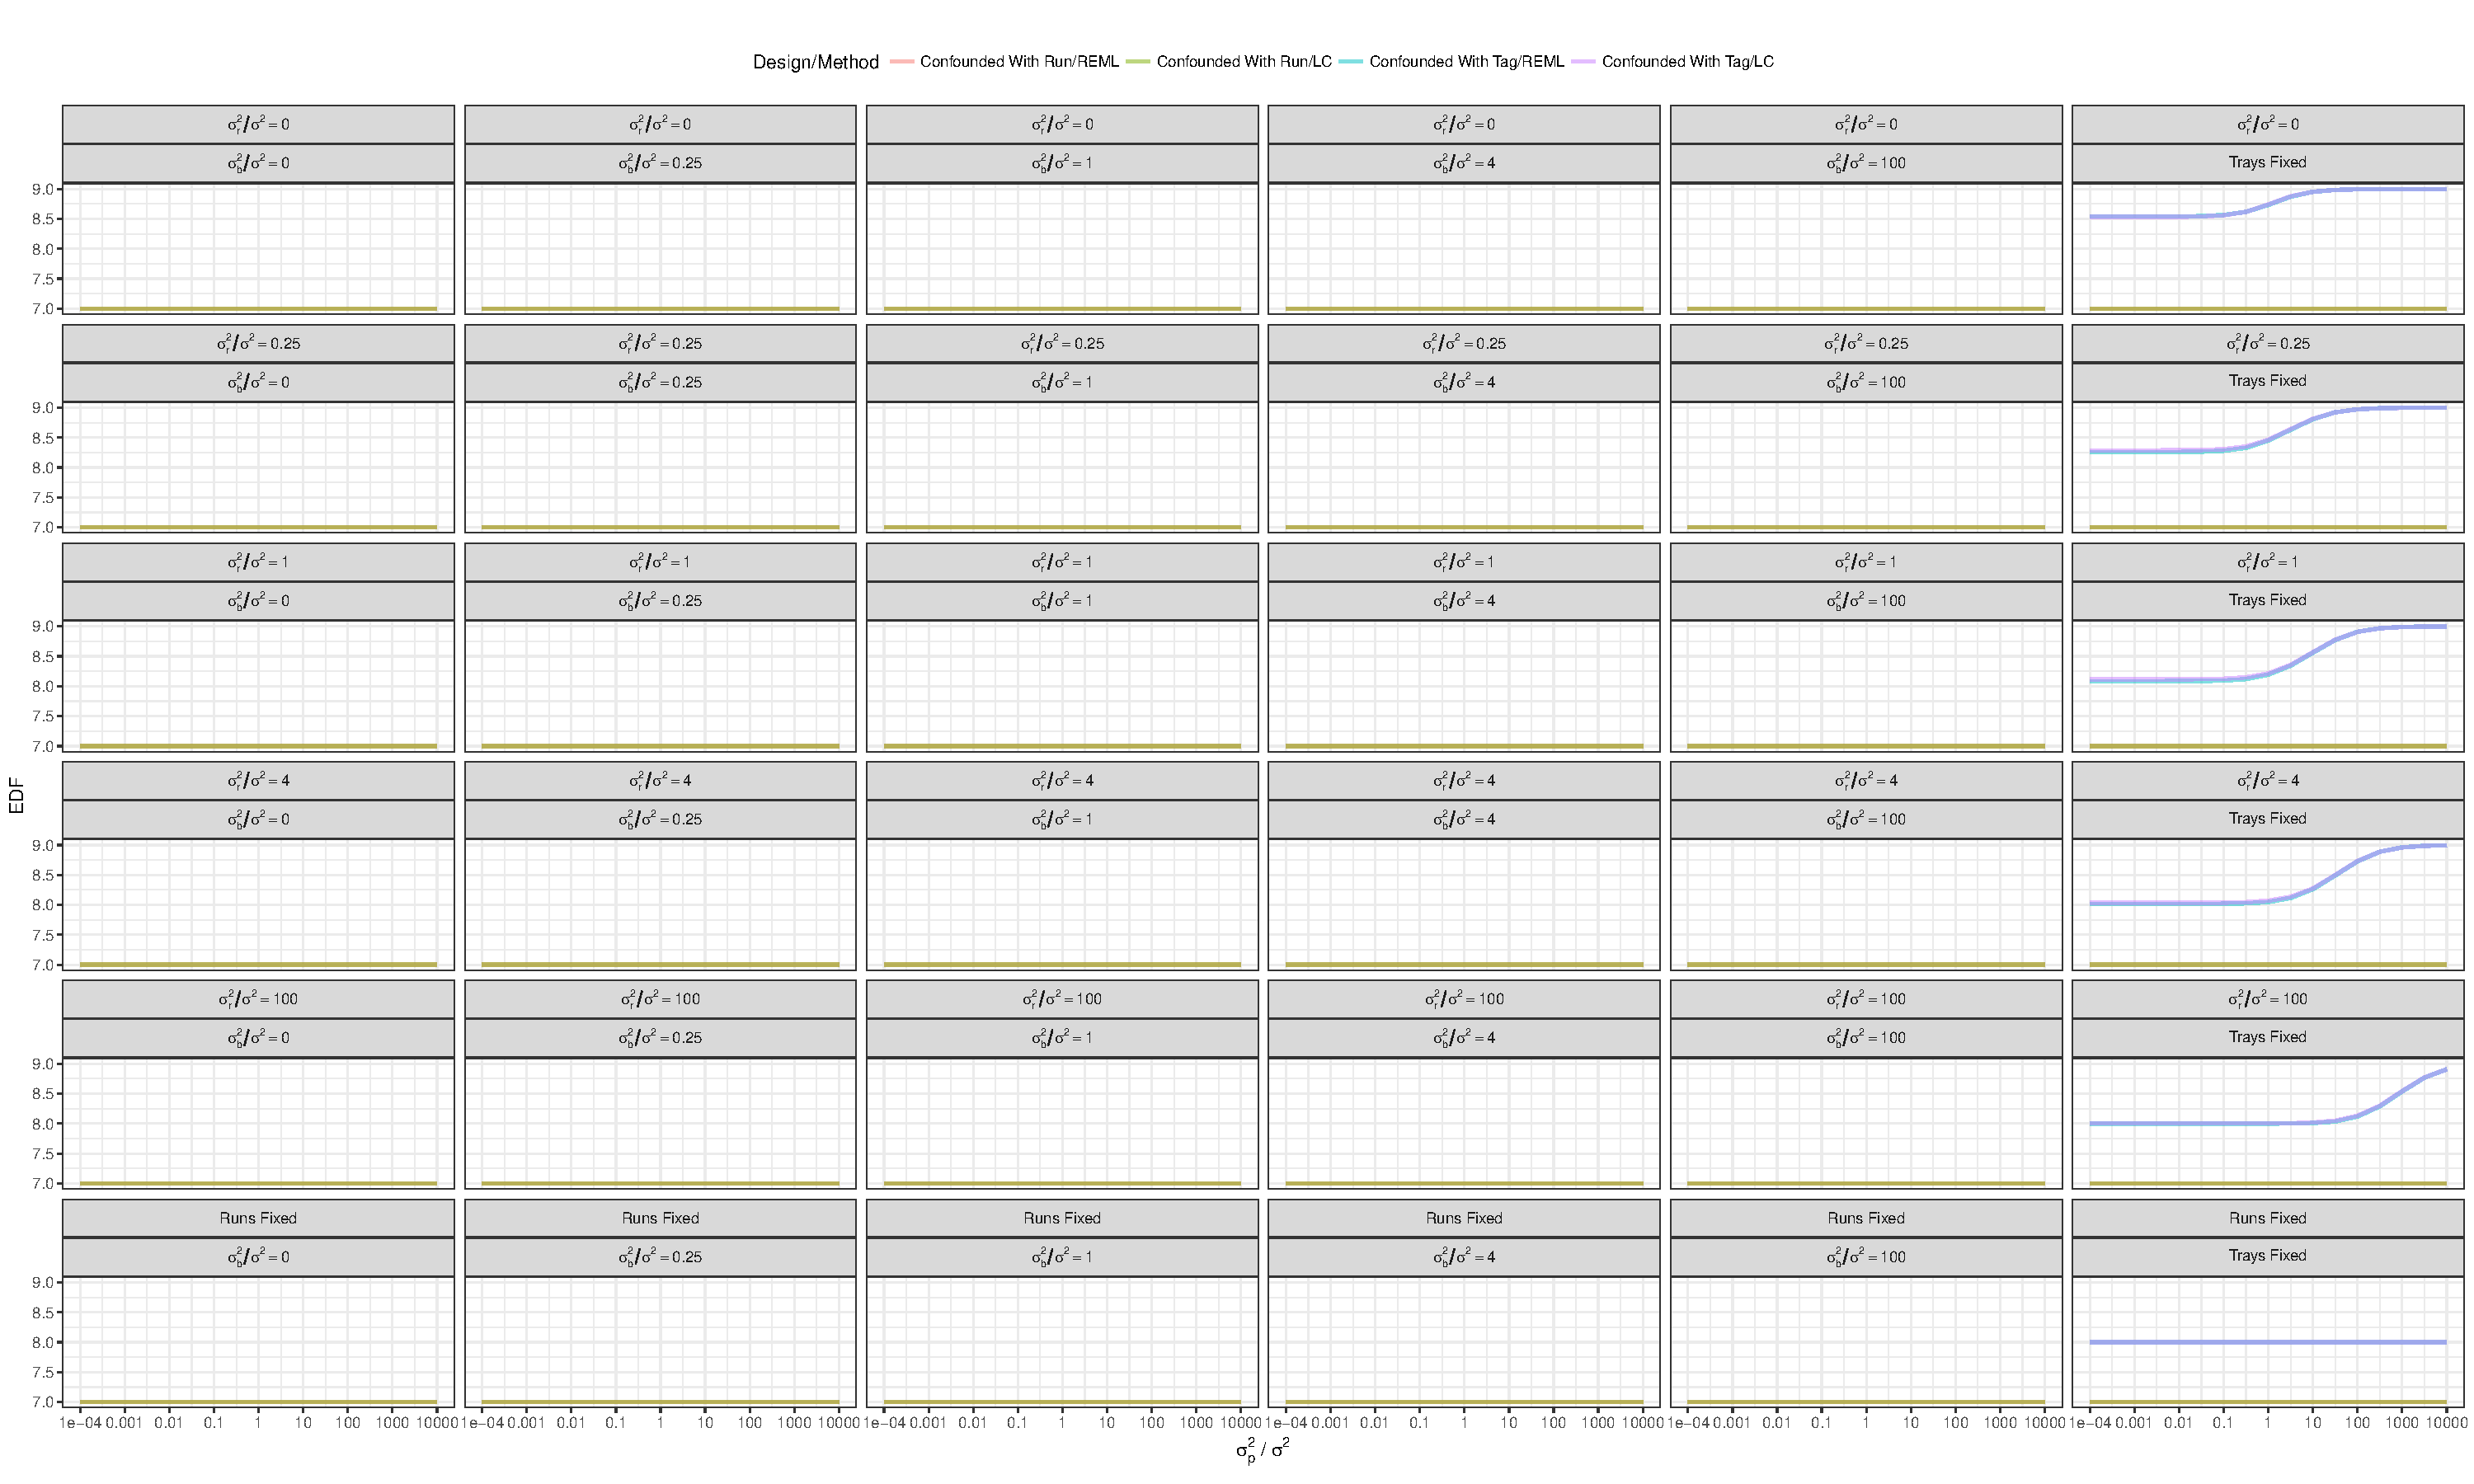
\includegraphics[width=1.3 \textwidth]{Chapter5/Graph/CRD44428.pdf}
\caption{EDF plots for optimal designs shown in Tables~\ref{tab:aniTrayDes3EDF} and \ref{tab:aniTrayDes4EDF}, where EDF is calculated using VCs estimated by both the REML and LC methods.}
\label{fig:RCBD442Tag8EDF}
\end{figure}
\end{landscape}

\subsection{Four-plex versus Eight-plex system}
From Figures~\ref{fig:RCBD442Tag4EDF} and ~\ref{fig:RCBD442Tag8EDF}, different ranges of values of the Between Tray VCs to measurement error ratio, denoted by $\sigma_{b}^2/\sigma^2$, did not change the EDF, because no extra information on the Between Plants VCs can be recovered from the Residual MS of the Between Tray Within Runs stratum and the Between Tray Within Runs stratum. Thus, Figure~\ref{fig:RCBD442Tag4vsTag8} only presents the EDF when Tray effects are assumed to be fixed, i.e.\ $\sigma_{b}^2 = \infty$, to make an overall comparison between the four- and eight-plex systems. 

Figure~\ref{fig:RCBD442Tag4vsTag8} shows the design when Tray effects are intentionally confounded with Tag effects with the eight-plex system being superior over the other three Phase 2 design options. However, there are three occasions when the EDF are the same between designs when Tray effects are intentionally confounded with Tag effects using the eight-plex system, and the design when Tray effects are intentionally confounded with Run effects using the four-plex system. The first occasion is when $\sigma_{r}^2/\sigma^2 = 4$ and $\sigma_{p}^2/\sigma^2$ is less than $0.1$, thus, run-to-run variation is 40 times that of plant-to-plant variation. The second occasion is when $\sigma_{r}^2/\sigma^2 = 100$ and  $\sigma_{p}^2/\sigma^2$ is less than 10, thus the run-to run variation is 10 times that of the plant-to-plant variation. The last occasion is when the Run effects are assumed to be fixed. Hence, the four-plex system will have the same precision as the eight-plex system when the run-to-run variation is 10 times higher than the plant-to-plant variation.  

\begin{figure}[h!]
\centering
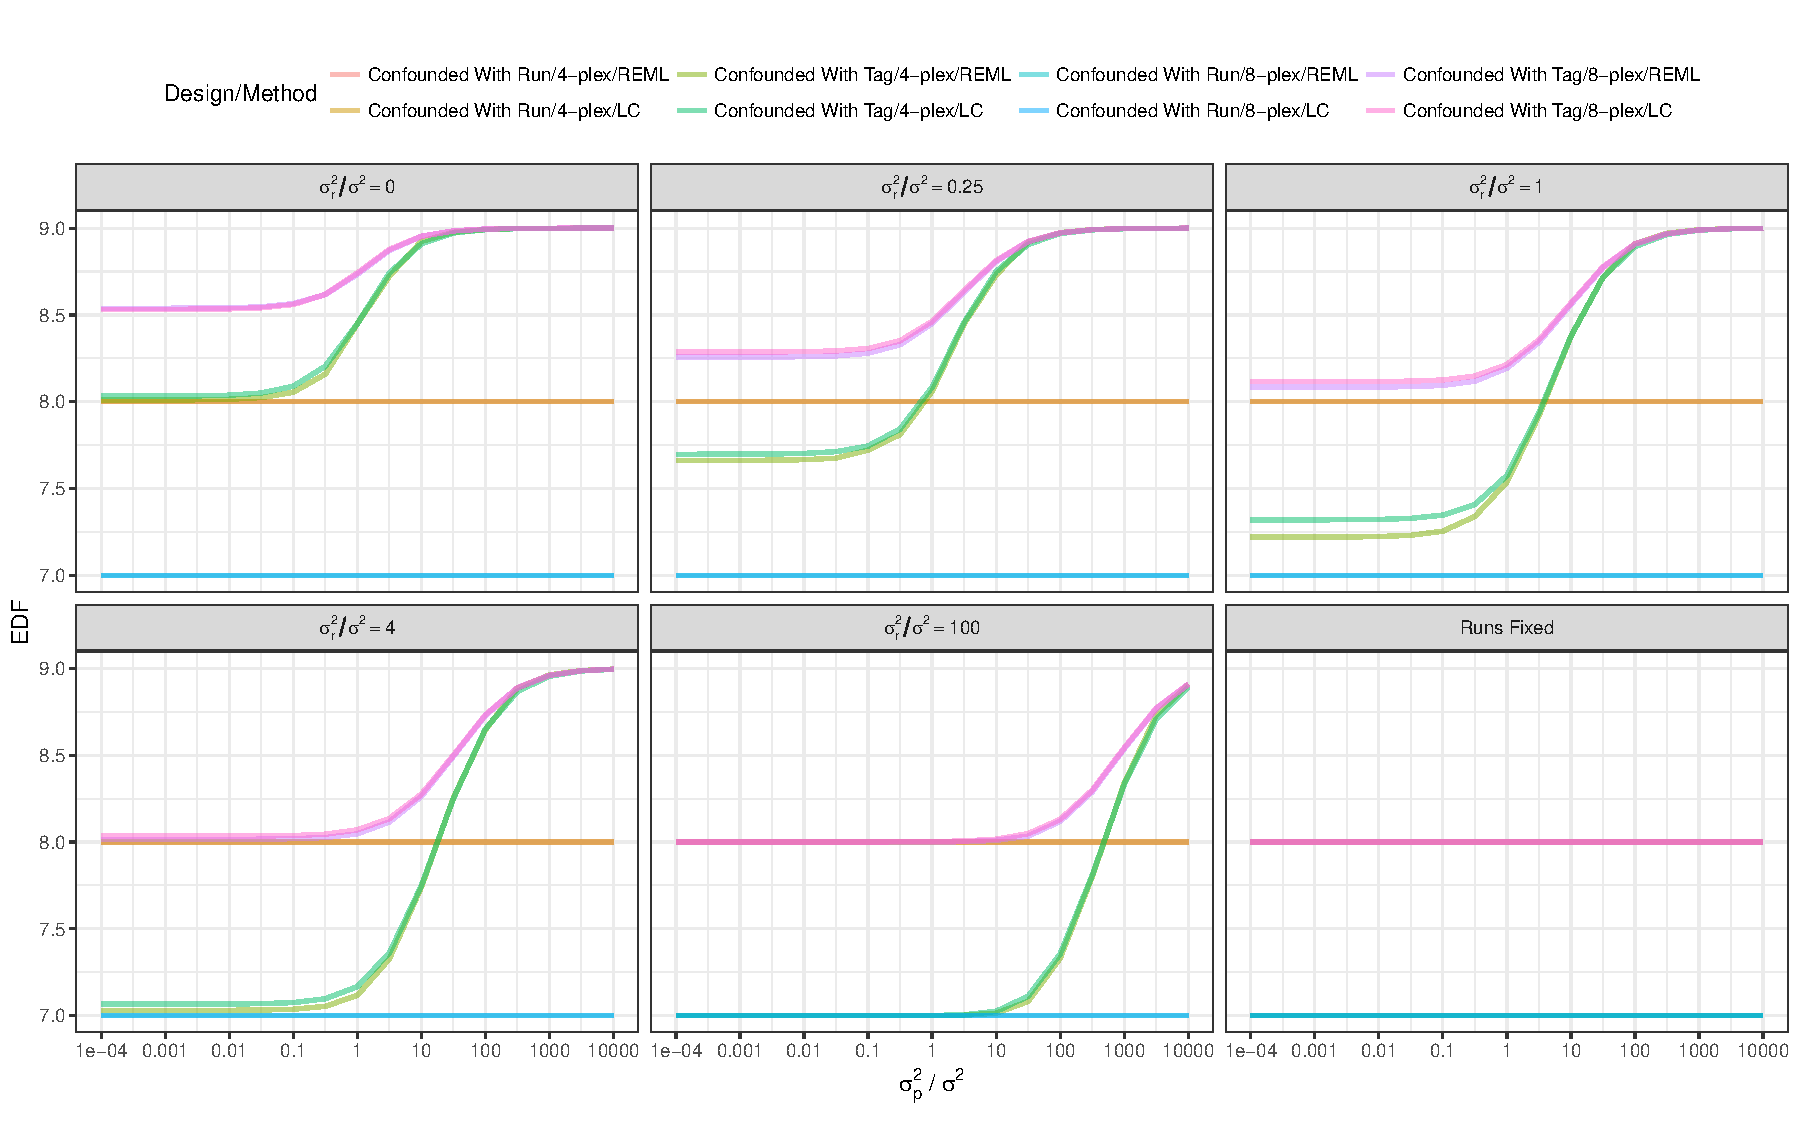
\includegraphics[width=1 \textwidth]{Chapter5/Graph/CRD44424vs8.pdf}
\caption{EDF for optimal designs shown in Tables~\ref{tab:aniTrayDes1EDF}, \ref{tab:aniTrayDes2EDF}, ~\ref{tab:aniTrayDes3EDF} and \ref{tab:aniTrayDes4EDF}, with Tray effects are assumed to be fixed, where EDF is calculated using VCs estimated by both the REML and LC methods.}
\label{fig:RCBD442Tag4vsTag8}
\end{figure}


\section{Summary}
\label{sec:conclusionChap5}
The Chapter described methods in estimating the VCs and approximating the EDF of Phase 2 experiments. EDF indicate how well we estimate the variances of Treatment effects, i.e. the Residual MS of the Between Experimental units stratum. Thus, the higher the EDF the better the estimates of the variance of Treatment effects and the valid F-test of the Treatment effects. We use EDF as another property with which to compare different optimal designs of the Phase 2 experiment found in Chapters 3 and 4. 

From all the EDF plots, we have shown that the REML method described here did not improve the approximation of the EDF from the optimal designs found in Chapters 3 and 4. This is due to these optimal designs having the property when the Phase 1 experimental units to the Phase 2 Blocks are always balanced, which ensures that we always have a valid F-test for testing for Treatment effects. Thus, these optimal designs are robust to the VC estimation procedure.

Three different cases were described when each case consists of the same Phase 1 design arranged in a CRD, comparing between using four-and eight-plex systems. The first case showed the four-plex system always generates higher EDF than the eight-plex system under different ranges of the VCs ratios. The second case showed when the EDF are always the same under different ranges of VCs ratios, because Treatment effects are completely confounded with Phase 2 Run effects, thus, the Run effects have to be assumed to be fixed. The last case showed an example when the four-plex system can have higher EDF than the eight-plex system, with run-to-run variation being higher than animal-to-animal variation, but the eight-plex system becomes better, with higher EDF, than the four-plex system when the animal-to-animal variation dominates.

The last part of the comparison was on the four different types of Phase 2 design with the same Phase 1 design arranged in a RCBD. These four different types of Phase 2 design comprised four-and eight-plex systems with two different confounding schemes when the Phase 1 Block (Tray) effects are intentionally confounded with the Phase 2 Tag and Run effects. We first showed that different ratios of Between Trays VCs to measurement error have no effects on the EDF. Further, the design when Phase 1 Block (Tray) effects are intentionally confounded with the Phase 2 Tag effects using the eight-plex system is preferable, as it generates the highest EDF among the four designs under all different combinations of the VCs. 



\chapter{Discussion}
\section{Summary}
The primary purpose of this study was to develop a method for the computer generation of optimal designs of two-phase multiplex proteomics experiments. This method for generating optimal designs uses a combination of theory to define objective functions and computing, to improve the simulated annealing (SA) algorithm. Since designs are computer generated, there is no restriction on the design parameters (of the Phase 1 experiment), and end-users do not need to be expert in designing experiments to use this tool to generate their design.    

The first part of this thesis applied the method of information decomposition to the design of any single- and two-phase experiment, and automated the construction of theoretical ANOVA tables. For single-phase experiments, the decomposition method was straightforward, as once the strata were defined based on the block structure, the treatment structure was then decomposed within each stratum. In two-phase experiments, however, decomposition began with the strata corresponding to the block structure in the Phase 2 experiment, followed by decomposition of the treatment structure into the strata corresponding to the Phase 1 experiment block structure. The procedure for the Phase~1 block-information decomposition was undertaken by regarding the Phase~1 block factors just as we would treatment factors. 

The method for applying information decomposition to designs of any single- and two-phase experiments is implemented in a newly developed \textsf{R} package called \pkg{infoDecompuTE} which is available on the Comprehensive \textsf{R} Archive Network (CRAN). This \textsf{R} Package allows the user to automate the construction of theoretical ANOVA tables to enable fast assessment of the attributes of designs. These attributes are the degrees of freedom (DF), expected mean squares (EMS), along with the variance components, fixed effects components, and the treatment average efficiency factor for every source of variation. 

For researchers who have no \textsf{R} experience, a Shiny application for the \pkg{infoDecompuTE} package is hosted at:
\url{https://kcha193.shinyapps.io/infoDecompuTE_Shiny/}. There are three type of outputs that can be generated from this Shiny application: 1) output from the \proglang{R} console as a text file, 2) latex code as a text file, and 3) latex compiled portable document format file. 

The second part of this thesis described a computational approach for finding optimal designs for Phase 2 proteomics experiments using MudPIT-iTRAQ$^{\rm TM}$ technologies. Chapter 3 presented the Phase 1 experiment arranged in a completely randomised design (CRD). The objective function was constructed to minimise confounding between Phase 1 Experiment units and Treatment effects with Phase 2 Run and Tag effects. The information matrix was constructed with an orthogonal projection matrix which projects $\bm{y}$ onto the Within Runs and Tags vector subspace, by assuming that Tag effects are random.

A three-criterion objective function was derived for generating the optimal design with three properties: 
\begin{enumerate}
\item information of the Phase 1 Experimental Units is maximised in the Within Runs stratum, based on A-optimal criteria,
\item treatment information is maximised in the Between Experimental Units Within Runs stratum, based on A-optimal criteria, and 
\item DF of the Treatment effects must still be intact in the Between Experimental Units Within Runs stratum.
\end{enumerate}

The modified nested SA algorithm presented consisted of two further improvements. The first improvement was applying the swapping method to only two of the experimental units of the Phase 1 experiment instead of the observational units. The second improvement was the three-stage swapping procedure, which divides a single large search space into three smaller search spaces, swapping the experiment units: 1) within the same runs, 2) within the same tags, and 3) not within the same runs and tags. These improvements were aimed at speeding up the process by optimising the objective function and then obtaining the optimal design. 

Chapter 4 extended the concept to finding the optimal design when the Phase 1 experiment is arranged in blocks, more specifically, a randomised complete block design (RCBD), or a balanced incomplete block design (BIBD). Having this additional Block factor from the Phase 1 experiment required us to adjust the objective function to have another criterion in maximising the Residual DF in the Between Plots Within Blocks Within Runs stratum. In addition, instead of having a single equation combining these four criteria with some weights, we optimise this new four-criterion objective function with three incremental steps:
\begin{enumerate}
\item The first step is to locate designs in which the Phase 1 Plots average efficiency factor in the Within Blocks Within Runs and Tags vector subspace equals 1, and the DF associated with Treatment effects in the Between Plots Within Blocks Within Runs stratum are intact.
\item Then from among the designs located in the first step, the second step uses the modified nested SA algorithm to find optimal designs in which the Residual DF in the Between Plots Within Blocks Within Runs stratum are maximised.
\item From among the designs found in the second step, the third step is to find the optimal design in which the treatment average efficiency factor in the Between Plots Within Blocks Within Runs and Tags vector subspace is maximised.
\end{enumerate}

Furthermore, two different types of confounding schemes were investigated, where Phase 1 Block effects are intentionally confounded with Tag effects, and where Phase 1 Block effects were intentionally confounded with Run effects. In general, designs in which Phase 1 Block effects were intentionally confounded with Tag effects were shown to have higher Residual DF in the Between Plots Within Blocks Within Runs stratum, because some DF associated with Tag effects were then estimated in the Between Block stratum. 

From the optimal designs generated, it was found that, if the Phase 1 experiment was arranged in a CRD with fewer than 16 animals (experimental units), it was better to use the four-plex system instead of the eight-plex system, due to the two extra DF available in the Between Animals Within Runs stratum. However, when more Phase 1 animals (experimental units) were used, the degrees of confounding between Animal effects and Run effects increased in the Phase 2 experiment; thus, it became preferable to use the eight-plex system over the four-plex system. In general, if the Phase 1 experiment is arranged in Blocks, it is recommended that the four-plex system should still be used when there are fewer than 16 animals (experimental units). However, no clear cut-off number of experimental units was identified, at which the eight-plex system become better than the four-plex system. This is because having the additional Block component could generate designs with higher Residual DF when Blocks effects that confounded with Tag effects. 

The main purpose of Chapters 3 and 4 was to describe the development of an automated process for finding the optimal design for a wide range of two-phase multiplexing experiments. Even though the main examples were comprise of four- and eight-plex experiments, the methods presented were more general and could be applied to all two-phase designs. This allows researchers using these technologies to design their experiments without requiring expert knowledge in experimental design. In addition, having this tool available also allows the consulting statisticians to present a quick solution to their client. (A set of resulting optimal designs were presented in Appendices~\ref{append:optimalCRDDes}, \ref{append:optimalRBDDes} and \ref{append:optimalBIBDDes}, and their properties were presented as tables in Appendices~\ref{append:optimalCRD}, \ref{append:optimalRBD} and \ref{append:optimalBIBD}.) 

The last part of the thesis showed how to estimate the variance components (VCs) using a restricted maximum likelihood (REML) when the Phase 2 Run effects are assumed to be random. We then showed how to approximate the effective degrees of freedom (EDF), which indicated how well we estimate the variances of Treatment effects, i.e. the residual MS of the stratum associated with the experimental unit. A design with higher EDF provided a better estimated of the variance of Treatment effects. However, the REML method described here did not improve the approximation of the EDF from the optimal designs found in Chapters 3 and 4. This was due to these optimal designs having the characteristic of balanced arrangement for Phase 1 experimental units to the Phase 2 Blocks, which ensured that we always had a valid F-test for testing Treatment effects. Thus, these optimal designs were robust to the VCs estimation procedure. 
 
\section{Future lines of research}
\subsection{Shiny application for generating optimal designs of Phase 2 experiments}
%%%%%%%%%%%%%%%%%%%%%%%%%%%%%%%%%%%%%%%%%%%%%%%%%%%%%%%%%%%%%%%%%%%
%Optimal designs 
%%%%%%%%%%%%%%%%%%%%%%%%%%%%%%%%%%%%%%%%%%%%%%%%%%%%%%%%%%%%%%%%%%%%%
Scientists are very adaptive at using these technologies, and they also have a good intuitive sense of needing to design their experiments to protect against unwanted systematic sources of variation. The introduction of labelling technologies in multiplexing for the ``omics'' experiments is evidence of this.

In Appendices~\ref{append:optimalCRDDes}, \ref{append:optimalRBDDes} and \ref{append:optimalBIBDDes}, we provided a set of designs that were generated from the work in Chapters 3 and 4. Researchers can used these to match their design parameters and select a design for their two-phase experiment.

Some additional \textsf{R} functions for the optimisation algorithm have been written, which will be published as a publicly available package on CRAN. Furthermore, this \textsf{R} package will also be turned into a Shiny application, so that it is easily accessible to end-users from a wide range of scientific disciplines. Thus, even scientists who are unfamiliar with \textsf{R} will feel comfortable using this application with user-friendly interface, and our design methods will become publicly available to all researchers.

%%%%%%%%%%%%%%%%%%%%%%%%%%%%%%%%%%%%%%%%%%%%%%%%%%%%%%%%%%%%%%%%%%%%%%%%%%%%%%%
\subsection{Effective degrees of freedom versus average treatment efficiency factor}
Chapter 5 included an example of a Phase 1 experiment involving $\nu = 8$ treatments assigned to $n_a = 16$ animals. We compared the theoretical ANOVA from the designs of the Phase 2 experiment using four-plex and eight-plex in Tables~\ref{tab:EDFDiscuss1} and \ref{tab:EDFDiscuss2}. 

In Table~\ref{tab:EDFDiscuss1}, when the Phase 2 experiment used the four-plex system, there were 3 DF associated with the Treatment effects estimated in the Between Runs stratum, with a treatment efficiency factors of $0.3$. Thus, the Run effects were assumed to be fixed, because we could not recover the extra information on Between Animals VC, $\sigma_a^2$,from the MS in the Between Animals Between Run stratum for estimating the variance of the Treatment effects. Hence, the EDF of the Between Animal Within Run stratum in this case were always 4 DF. As in Table~\ref{tab:EDFDiscuss1} when the Phase 2 experiment used the eight-plex system, confounding occurred between Treatment and Tag effects, with Tag effects containing $0.3$ of the treatment information. Since the Run effects were assumed as random, we could recover the extra information from the Between Animals Between Runs stratum for estimating the variance of Treatment effects, thus the EDF could be as high as 5 DF.   

\begin{table}[!ht]
\centering
 \caption{Theoretical ANOVA table from the Phase 1 experiment arranged in CRD with $\nu = 8$ and $r_b = 2$, and from the Phase 2 experiment using the four-plex system.}
 \begin{tabular}[t]{lrlll} 
 \toprule 
 \multicolumn{1}{l}{\textbf{Source of Variation}} & \multicolumn{1}{l}{\textbf{DF}} & \multicolumn{1}{l}{\textbf{EMS}}& \multicolumn{1}{l}{$\bm{E_{\gamma}}$}&\multicolumn{1}{l}{$\bm{E_{\tau}}$}\\ 
 \midrule 
 Between Runs &  &  & & \\ 
 \quad Between Animals &  &  & & \\ 
 \quad \quad Treatment & $3$ & $\sigma^2+2\sigma_{a}^2+4\sigma_{r}^2+1.2\theta_{\tau}$ & & $0.3$\\ 
 \quad Within Animals & $4$ & $\sigma^2+4\sigma_{r}^2$ & & \\ \hline 
 Within Run &  &  & & \\ 
 \quad Between Animals &  &  & & \\ 
 \quad \quad Tag & $1$ & $\sigma^2+2\sigma_{a}^2+8\theta_{\gamma}$ &$1$ & \\ 
 \quad \quad Treatment & $7$ & $\sigma^2+2\sigma_{a}^2+ 3.23\theta_{\tau}$ & & $0.8077$\\ 
 \quad \quad Residual & $4$ & $\sigma^2+2\sigma_{a}^2$ & & \\ \hline 
 \quad Within Animals &  &  & & \\ 
 \quad \quad Tag & $2$ & $\sigma^2+8\theta_{\gamma}$ &$1$ & \\ 
 \quad \quad Residual & $10$ & $\sigma^2$ & & \\ 
 \bottomrule 
 \end{tabular} 
 \label{tab:EDFDiscuss1}
\end{table} 

\begin{table}[!ht]
\centering
 \caption{Theoretical ANOVA table from the Phase 1 experiment arranged in CRD with $\nu = 8$ and $r_b = 2$ and the Phase 2 experiment using the eight-plex system.}
 \begin{tabular}[t]{lrlll} 
 \toprule 
 \multicolumn{1}{l}{\textbf{Source of Variation}} & \multicolumn{1}{l}{\textbf{DF}} & \multicolumn{1}{l}{\textbf{EMS}}& \multicolumn{1}{l}{$\bm{E_{\gamma}}$}&\multicolumn{1}{l}{$\bm{E_{\tau}}$}\\ 
 \midrule 
 Between Runs &  &  & & \\ 
 \quad Between Animals & $1$ & $\sigma^2+2\sigma_{a}^2+8\sigma_{r}^2$ & & \\ 
 \quad Within Animals & $2$ & $\sigma^2+8\sigma_{r}^2$ & & \\ \hline 
 Within Runs &  &  & & \\ 
 \quad Between Animals &  &  & & \\ 
 \quad \quad Tag & $3$ & $\sigma^2+2\sigma_{a}^2+4\theta_{\gamma}+1.2\theta_{\tau}$ &$1$ &  $0.3$\\ 
 \quad \quad Treatment & $7$ & $\sigma^2+2\sigma_{a}^2+3.23\theta_{\tau}$ & & $0.8077$\\ 
 \quad \quad Residual & $4$ & $\sigma^2+2\sigma_{a}^2$ & & \\ \hline 
 \quad Within Animals &  &  & & \\ 
 \quad \quad Tag & $4$ & $\sigma^2+4\theta_{\gamma}$ &$1$ & \\ 
 \quad \quad Residual & $10$ & $\sigma^2$ & & \\ 
 \bottomrule 
 \end{tabular} 
 \label{tab:EDFDiscuss2}
\end{table} 

Additional work can be done in comparing between recovering the treatment information across runs, and recovering the extra DF in EDF to get a better estimate of the variance. To achieve this, it would mean performing more extensive simulation studies to understand which of these two designs would be preferable and under which circumstances. These circumstances are not just different ranges of values of VCs, but also different ranges of values in the fixed effects for the simulation study. 

%%%%%%%%%%%%%%%%%%%%%%%%%%%%%%%%%%%%%%%%%%%%%%%%%%%%%%%%%%%%%%%%%%%%%%%%%%%%%%%
\subsection{Missing values}
One of the issues that arises with high-throughput multiplexing experiments is that of missing data. For a single protein, there are various ways in which missing values can arise in a MudPIT-iTRAQ$^{\rm TM}$ proteomics experiment. One form of missing data in which we are most interested, is when a unique peptide, which only belongs to a specific protein, is simply not found in one run of the experiment, but can be found on the other runs of the experiment. Thus, during database searching, bioinformatics software cannot re-construct this specific protein; and this protein would then be considered as missing for one entire run of the Phase 2 experiment. This can be problematic in the analysis stage, as the design is likely to become unbalanced due to unequal replication of the treatment group or the experimental units from the Phase 1 experiment.  
 
For example, consider the Phase 2 experiment with the Phase~1 experiment consisting of $\nu = 4$ treatments assigned to $n_a = 12$ animals. Each animal is then further split into $n_s = 2$ sub-samples and measured in the Phase 2 MudPIT-iTRAQ$^{\rm TM}$ experiment comprising $n_r = 6$ runs and $n_\gamma = 4$ tags. An optimal design of Phase 2 experiment or this scenario is presented in Table ~\ref{tab:DesCon}. 

\begin{table}[ht]
\centering
\itshape
\caption{Optimal design for Phase 2 experiment showing the allocation of sub-samples from treatments assigned to animals, when the Phase~1 experiment consists of $\nu = 4$ treatments assigned to $n_a = 12$ animals, $n_s = 2$ sub-samples are then taken from each animals and measured in the Phase 2 MudPIT-iTRAQ$^{\rm TM}$ experiment comprising $n_r = 6$ runs and $n_\gamma = 4$ tags.}
\begin{tabular}[t]{c|cc:cc}
 & \multicolumn{4}{c}{{\bf Tag}} \\
{\bf Run}  & \textnormal{114} & \textnormal{115} & \textnormal{116} & \textnormal{117} \\  
\hline 
\textnormal{1} & Jb & Ld & Ea & Cc \\ 
\textnormal{2} & Ld & Jb & Cc & Ea \\ 
\textnormal{3} & Aa & Gc & Fb & Dd \\ 
\textnormal{4} & Gc & Aa & Dd & Fb \\ 
\textnormal{5} & Hd & Ia & Kc & Bb \\ 
\textnormal{6} & Ia & Hd & Bb & Kc \\ 
\end{tabular}
 \label{tab:DesCon} 
\end{table}

The theoretical ANOVA of the full design in Table~\ref{tab:DesCon} is presented in Table~\ref{tab:Full}. The total of 23 DF were partitioned to 5 DF for Between Runs stratum and 18 DF for Within Runs stratum. In the Between Animals Within Runs stratum, Treatment effects could be estimated with $0.96$ amount of the treatment information with 5 Residual DF for estimating the variance of Treatment effects. In addition, there was a valid F-test for comparing between treatments, because the coefficients of VCs were the same for the Treatment and Residual EMS in the Between Animals Within Runs stratum.

\begin{table}[!ht]
\centering
 \caption{Theoretical ANOVA table of design in Table~\ref{tab:DesCon}. }
\begin{tabular}[t]{lrlll} 
\toprule 
\multicolumn{1}{l}{\textbf{Source of Variation}} & \multicolumn{1}{l}{\textbf{DF}} & \multicolumn{1}{l}{\textbf{EMS}}&\multicolumn{1}{l}{$\bm{E_{\gamma}}$}&\multicolumn{1}{l}{$\bm{E_{\tau}}$}\\ 
\midrule 
Between Runs &  &  & & \\ 
\quad Between Animals & $2$ & $\sigma^2+2\sigma_{a}^2+4\sigma_{r}^2$ & & \\ 
\quad Within Animals & $3$ & $\sigma^2+4\sigma_{r}^2$ & & \\ \hline 
Within Runs &  &  & & \\ 
\quad Between Animals &  &  & & \\ 
\quad \quad Tag & $1$ & $\sigma^2+2\sigma_{a}^2+6\theta_{\gamma}+0.67\theta_{\tau}$ &$1$ & $0.1111$\\ 
\quad \quad Treatment  & $3$ & $\sigma^2+2\sigma_{a}^2+5.76\theta_{\tau}$ & & $0.96$\\ 
\quad \quad Residual & $5$ & $\sigma^2+2\sigma_{a}^2$ & & \\ \hline 
\quad Within Animals &  &  & & \\ 
\quad \quad Tag & $2$ & $\sigma^2+6\theta_{\gamma}$ &$1$ & \\ 
\quad \quad Residual & $7$ & $\sigma^2$ & & \\ 
\bottomrule 
 \end{tabular} 
 \label{tab:Full} 
\end{table}

If a given protein was not detected in Run 6, then there would be four observations missing for the Phase 2 experiment. The theoretical ANOVA is presented Table~\ref{tab:MissingOneRun}, which shows that the total DF are reduced to 19 DF. The Residual DF in the Between Animals Within Runs stratum are also reduced to 3 DF, which is 2 DF less than the full design. Furthermore, there is no direct valid F-test for this design, as coefficients of the VCs from the Treatment and Residual EMS are different in the Between Animals Within Runs stratum. Finally, the amount of the treatment information is also reduced from $0.96$ to $0.8$. 

\begin{table}[!ht]
\centering
 \caption{Theoretical ANOVA table of design in Table~\ref{tab:DesCon} with Run 6 missing.}
\begin{tabular}[t]{lrlll} 
\toprule 
\multicolumn{1}{l}{\textbf{Source of Variation}} & \multicolumn{1}{l}{\textbf{DF}} & \multicolumn{1}{l}{\textbf{EMS}}&\multicolumn{1}{l}{$\bm{E_{\gamma }}$}&\multicolumn{1}{l}{$\bm{E_{\tau}}$}\\ 
\midrule 
Between Run &  &  & & \\ 
\quad Between Animals & $2$ & $\sigma^2+ 1.6\sigma_{a}^2+4\sigma_{r}^2$ & & \\ 
\quad Within Animals & $2$ & $\sigma^2+4\sigma_{r}^2$ & & \\ \hline 
Within Run &  &  & & \\ 
\quad Between Animals &  &  & & \\ 
\quad \quad Tag & $3$ & $\sigma^2+1.27\sigma_{a}^2+1.36\theta_{\gamma}+0.43\theta_{\tau}$ &$0.2727$ & $0.0857$\\ 
\quad \quad Treatment & $3$ & $\sigma^2+1.96\sigma_{a}^2+4.23\theta_{\tau}$ & & $0.8471$\\ 
\quad \quad Residual & $3$ & $\sigma^2+1.78\sigma_{a}^2$ & & \\ \hline 
\quad Within Animals &  &  & & \\ 
\quad \quad Tag & $2$ & $\sigma^2+4\theta_{\gamma}$ &$0.8$ & \\ 
\quad \quad Residual & $4$ & $\sigma^2$ & & \\ 
\bottomrule 
 \end{tabular} 
 \label{tab:MissingOneRun} 
\end{table}

If a given protein is not detected in Runs 5 and 6, we then are left with 16 observations for the Phase 2 experiment. The theoretical ANOVA of the new design is presented in Table~\ref{tab:MissingTwoRuns}. The Residual DF in the Between Animals Within Runs stratum is reduced to 2 DF, which is 3 DF less than the full design. However, there is a valid F-test for Treatment effects, with Treatment effects being fully estimable in the Between Animals Within Runs stratum. This is due to the way that we structured our initial designs with a 2-run-by-2-tag array system. Hence, if the last two runs of the experiment were to be missing, we basically lose one biological replicate, i.e.\ there would now be 8 animals from the Phase 1 experiments, so that the allocation of sub-samples of animals and treatments, to be labelled with tags and analysed with runs still would have a balanced arrangement. Hence, the optimal design presented in Table~\ref{tab:DesCon} is shown to be robust in dealing with certain patterns of missing data, i.e.\ when Runs 1 and 2, or Runs 3 and 4, or Runs 5 and 6 are missing. Other different patterns of missing data will result in designs that have no valid F-test for treatment effects, or will make it difficult to estimate the VCs from the theoretical ANOVA.   

\begin{table}[!ht]
\centering
 \caption{Theoretical ANOVA table of design in Table~\ref{tab:DesCon} with Runs 5 and 6 missing.}
\begin{tabular}[t]{lrlll} 
\toprule 
\multicolumn{1}{l}{\textbf{Source of Variation}} & \multicolumn{1}{l}{\textbf{DF}} & \multicolumn{1}{l}{\textbf{EMS}}&\multicolumn{1}{l}{$\bm{E_{\gamma}}$}&\multicolumn{1}{l}{$\bm{E_{\tau}}$}\\ 
\midrule 
Between Run &  &  & & \\ 
\quad Between Animals & $1$ & $\sigma^2+2\sigma_{a}^2+4\sigma_{r}^2$ & & \\ 
\quad Within Animals & $2$ & $\sigma^2+4\sigma_{r}^2$ & & \\ \hline 
Within Run &  &  & & \\ 
\quad Between Animals &  &  & & \\ 
\quad \quad Tag & $1$ & $\sigma^2+2\sigma_{a}^2+4\theta_{\gamma}$ &$1$ & \\ 
\quad \quad Treatment & $3$ & $\sigma^2+2\sigma_{a}^2+4\theta_{\tau}$ & & $1$\\ 
\quad \quad Residual & $2$ & $\sigma^2+2\sigma_{a}^2$ & & \\ \hline 
\quad Within Animals &  &  & & \\ 
\quad \quad Tag & $2$ & $\sigma^2+4\theta_{\gamma}$ &$1$ & \\ 
\quad \quad Residual & $4$ & $\sigma^2$ & & \\ 
\bottomrule 
 \end{tabular} 
 \label{tab:MissingTwoRuns} 
\end{table} 
 
Further simulation studies can be done to explore what happens to the properties of the designs considered in Chapters 3 and 4 with different patterns of missingness. We may investigate how the design can start to break down as observed in Table~\ref{tab:MissingOneRun}, when there is one run of the experiment that is missing. We can further examine any alternative designs which have more desirable properties in terms of their robustness for downstream statistical analyses when we have missing values.

An alternative approach would be to construct an imputation model under a Bayesian multivariate and multilevel inference framework \citep{Zeng2017}. This model would use the information from experimental factors, such as the physical properties of the peptides, the effects from iTRAQ$^{\rm TM}$ tags and MudPIT runs, along with the clinical factors of each patient to construct a likelihood model. Each parameter in the likelihood model would be estimated using an Empirical Bayesian Hamiltonian MC algorithm, which integrates prior information for missing data and the distribution of missing values. The resultant posterior distribution of these parameters, including parameters of interest, would therefore be estimated utilising both the pattern of missing data and information for missing values. We could incorporate this framework into how to better design the Phase 2 experiment, which would enable us to impute reliable values for the final analysis.

\section{More general future research directions}
Another multiplexing technology, which started to become popular only a few years ago is \emph{Next-Generation Sequencing} (NGS). This multi-plexing technology can be carried out by attaching unique index sequences, namely \emph{barcodes}, onto the end of each DNA or RNA fragment \citep{smith2010}. Therefore, different barcodes are attached to different biological samples, allowing an NGS instrument to sequence multiple samples simultaneously. The abundance levels of sequences are then measured based on the number of barcodes present in each sample. These barcodes are very similar to the iTRAQ$^{\rm TM}$ tags used when measuring protein abundances. Note that MudPIT runs of the proteomics experiments are referred to as \emph{lanes} of the NGS experiments. Thus, the methods of optimal designs described in this thesis also apply to this technology. 

We can currently obtain a kit with 96 and 384 barcodes, meaning that we can quantify up to 96 or 384 unique samples at the same time \citep{smith2010, Shapland2015}. However, using more barcodes is not always ideal, because as more barcodes are used the number of DNA or RNA sequences for each barcode decreases \citep{campbell2015}. Hence, deciding on the number of barcodes is more practical than theoretical. 

Let us consider a Phase 1 experiment arranged in a CRD with $\nu = 8$ treatments assigned to $n_a = 48$ animals, and the sample from each animal split into $n_s = 2$ sub-samples, which gives us a total of $n = 96$ sub-samples to be measured using the NGS technology. If a researcher decides to use the kit with 96 barcodes for just one lane of the experiment, then the Treatment effects are completely confounded with Tag effects. 

Using the objective function and SA algorithm derived in this thesis, we can quickly generate four optimal designs with multiple lanes, where all have a valid F-test for Treatment effects, with different numbers of barcodes used in the Phase 2 experiment. The Residual DF and the treatment average efficiency factors of these four designs are presented in Table~\ref{tab:NGS}. This shows that the best option is to use $8$ lanes of the experiment with $12$ barcodes, which generates the highest Residual DF (32 DF) and the treatment average efficiency factors ($0.9837$) in the Between Animals Within Runs stratum. However, given that each lane of experiment costs about five thousand dollars, it may be ideal to advise the researcher to use 4 lanes with $24$ barcodes, because there would not a lot of improvement compared to using $8$ lanes of the experiment with $12$ barcodes. Therefore, more work can be done in examining the efficiency of using different numbers of barcodes for generating a better optimal design of the Phase 2 experiment.

\begin{table}[!h]
\centering
\caption{Residual DF and treatment average efficiency factors from the optimal design with different number of lanes and barcodes for Next-Generation Sequencing technology.}
\begin{tabular}{|l|l|l|l|}
\hline 
Number of lanes	& Number of barcodes & Residual DF & $E_\tau$  \\ 
\hline 
$2$ 	& $48$ & $17$ & $0.56$ \\ 
\hline 
$4$ 	& $24$ & $28$ & $0.8532$  \\ 
\hline 
$8$ & $12$ & $32$ & $0.9837$  \\ 
\hline 
$16$ & $6$ & $31$ & $0.9510$  \\ 
\hline 
\end{tabular} 
\label{tab:NGS}
\end{table}
 
Finally, the NGS experiment returns counts as the response. The method in this thesis assumes that the response, once log transformed, is normally distributed; thus, all of the designs we have generated assume unit-treatment additivity. Having a count as the response violates this assumption, and so further research could be undertaken on how to obtain optimal designs of the two-phase experiment where the response exhibits a non-normal distribution.

Further research outlined here will help to maximise the benefits of new technologies, such as NGS, while at the same time extending the capabilities of our method, for generating optimal designs, to a wider range of settings in two-phase multiplex proteomics experiments. 




\begin{appendices}
\chapter{Reference manual of infoDecompuTE package} \label{append:infoDecompuTE}

\includepdf[pages={1-},scale=1]{ChapterAppendix/infoDecompuTE.pdf}

\chapter{The Information matrix in more detail} \label{append:informatSym}
This Chapter is to show that the information matrix $\Z' (\I-\mP_{r})(\I -\mP_{\gamma}) \Z$ used for the objective function is symmetric. 

Let $\mP_r$ and $\mP_\gamma$ be orthogonal projection matrices, then 
\[
\mP_r = \mP_r^2 = \mP_r\mP_r \; \; \mathrm{and} \; \; \mP_r = \mP_r'
\]
So 
\begin{eqnarray}
\nonumber &&	\Z' (\I-\mP_{r})(\I -\mP_{\gamma}) \Z\\
\nonumber &=& 	\Z' (\I-\mP_{r} - \mP_{\gamma} + \mP_{r}\mP_{\gamma}) \Z\\
\nonumber &=&	\Z' \Z - \Z'\mP_{r} \Z  - \Z' \mP_{\gamma}\Z  + 2\Z' \mP_{r}\mP_{\gamma}\Z\\
\label{eq:informatSym} &=&	\Z' \Z - (\mP_{r}\Z)'\Z\mP_{r} - (\mP_{\gamma}\Z )'\mP_{\gamma}\Z  + 2\Z' \mP_{r}\mP_{\gamma}\Z\\
\end{eqnarray}
where $\Z' \Z$, $(\mP_{r}\Z)'\Z\mP_{r}$ and $(\mP_{\gamma}\Z )'\mP_{\gamma}\Z$ are symmetric. 

The projection matrix which projects $\bm{y}$ onto the Between Runs vector subspace is 
\[
\mP_{r} = \W_{r}(\W_{r}'\W_{r})^{-1} \W_{r}'
\]
where $\W_{r}$ is design matrix for Run factor of the Phase 2 experiment and can be expressed as 
\[
 \W_{r} = \mathbf{1}_{n_\gamma} \otimes \I{n_r}.
\]
Thus, projection matrix for Between Runs can be re-written as  
\[
\mP_{r} =\frac{1}{n_\gamma} \mathbf{1}_{n_\gamma}  \mathbf{1}_{n_\gamma}' \otimes \I{n_r}.
\]

The projection matrix which projects $\bm{y}$ onto the Between Tags vector subspace is 
\[
\mP_{\gamma} = \X_{\gamma}(\X_{\gamma}'\X_{\gamma})^{-1}\X_{\gamma}
\]
where $\X_{\gamma}$ is design matrix for Tag factor of the Phase 2 experiment and can be expressed as 
\[
\X_{\gamma} = \I{n_\gamma} \otimes \mathbf{1}_{n_r} 
\]
Thus, projection matrix for Between Tags can be re-written as  
\[
\mP_{\gamma} = \frac{1}{n_r} \I{n_\gamma} \otimes \mathbf{1}_{n_r}\mathbf{1}_{n_r}'.
\]

This follow by $\mP_{r}\mP_{\gamma}$ in \ref{eq:informatSym} becomes 
\begin{eqnarray}
\nonumber \mP_{r}\mP_{\gamma}  &=& \frac{1}{n_r n_\gamma}  \mathbf{1}_{n_\gamma}  \mathbf{1}_{n_\gamma}' \otimes \mathbf{1}_{n_r}\mathbf{1}_{n_r}'\\
\nonumber &=& \frac{1}{n}  \mathbf{1}_{n_\gamma n_r}  \mathbf{1}_{n_\gamma n_r}' \\
\nonumber &=& \frac{1}{n}  \mathbf{1}_{n}  \mathbf{1}_{n}' \\
\nonumber &=&	\K_{n}. \\
\end{eqnarray}
Thus,  $\mP_{r}\mP_{\gamma} = \K$, then
\[ \Z' \mP_{r}\mP_{\gamma}\Z =  \frac{1}{n} \Z' \mathbf{1} \mathbf{1}' \Z  = \frac{1}{n} (\Z' \mathbf{1}) (\Z' \mathbf{1})'. \] 

Let
\[Z = 
\begin{pmatrix}  
a_{11} & a_{12} & a_{13} \\
a_{21} & a_{22} & a_{23} \\             
a_{31} & a_{32} & a_{33} \\
\end{pmatrix},
\]
then
\[ Z' \mathbf{1} = 
\begin{pmatrix}  
a_{.1} \\
a_{.2}\\             
a_{.3}  \\
\end{pmatrix}.
\]
So, 
\begin{eqnarray}
\nonumber (\Z' \mathbf{1}) (\Z' \mathbf{1})' 
\nonumber &=& \begin{pmatrix}  
a_{.1} \\
a_{.2}\\             
a_{.3}  \\
\end{pmatrix}
 \begin{pmatrix}  
a_{.1} & a_{.2} & a_{.3}\\
\end{pmatrix} \\
\nonumber &=&\begin{pmatrix}  
a_{.1}^2 & a_{.1}a_{.2} & a_{.1}a_{.3} \\
a_{.2}a_{.1} & a_{.2}^2 & a_{.2}a_{.3} \\             
a_{.3}a_{.1} & a_{.3}a_{.2} & a_{.3}^2 \\
\end{pmatrix}. 
\end{eqnarray}
Thus, $\Z' \mP_{r}\mP_{\gamma}\Z$ is also symmetric.  

\chapter{Various matrices from the example in Section~\ref{sec:theorANOVAtab}} \label{append:theorANOVAtab}

The orthogonal projection matrix of Within Runs and Tags vector subspace is given by
\[
\Q_{r\gamma} = 
\begin{bmatrix} 
 0.38 & -0.12 & -0.12 & -0.12 & -0.38 & 0.12 & 0.12 & 0.12 \\ 
  -0.12 & 0.38 & -0.12 & -0.12 & 0.12 & -0.38 & 0.12 & 0.12 \\ 
  -0.12 & -0.12 & 0.38 & -0.12 & 0.12 & 0.12 & -0.38 & 0.12 \\ 
  -0.12 & -0.12 & -0.12 & 0.38 & 0.12 & 0.12 & 0.12 & -0.38 \\ 
  -0.38 & 0.12 & 0.12 & 0.12 & 0.38 & -0.12 & -0.12 & -0.12 \\ 
  0.12 & -0.38 & 0.12 & 0.12 & -0.12 & 0.38 & -0.12 & -0.12 \\ 
  0.12 & 0.12 & -0.38 & 0.12 & -0.12 & -0.12 & 0.38 & -0.12 \\ 
  0.12 & 0.12 & 0.12 & -0.38 & -0.12 & -0.12 & -0.12 & 0.38 \\ 
\end{bmatrix} . 
\]

The animal information matrix in the Within Runs and Tags vector subspace is given by 
\[
\A_{a} = 
 \Z_{a}' Q_{r\gamma} \Z_{a} = 
\begin{bmatrix} 
 1 & -1 & 0 & 0 \\ 
 -1 & 1 & 0 & 0 \\ 
 0 & 0 & 1 & -1 \\ 
 0 & 0 & -1 & 1 \\ 
\end{bmatrix}.  
\]


The treatment information matrix of animals in the Within Runs and Tags vector subspace is given by 
\[
\A_{\tau} = 
 \X_{a}' Q_{r\gamma} \X_{a} = 
\begin{bmatrix} 
 2 & -2 \\ 
 -2 & 2 \\ 
\end{bmatrix}.  
\]

\chapter{Various matrices from the example in Subsection~\ref{sub:compareMSvsA}} \label{append:compareMSvsA}


The animal information matrix in the Within Runs and Tags vector subspace of the MS-optimal design is given by 
\[
\A_{a} = 
 \Z_{a}' \Q_{r\gamma} \Z_{a} = 
\begin{bmatrix} 
 1.17 & -0.25 & -0.25 & -0.25 & -0.17 & -0.25 \\ 
 -0.25 & 1.17 & -0.25 & 0.08 & -0.25 & -0.50 \\ 
 -0.25 & -0.25 & 1.17 & -0.50 & -0.25 & 0.08 \\ 
 -0.25 & 0.08 & -0.50 & 1.17 & -0.25 & -0.25 \\ 
 -0.17 & -0.25 & -0.25 & -0.25 & 1.17 & -0.25 \\ 
 -0.25 & -0.50 & 0.08 & -0.25 & -0.25 & 1.17 \\ 
\end{bmatrix}.  
\]


The animal information matrix in the Within Runs and Tags vector subspace of the A-optimal design is given by 
\[
\A_{a} = 
 \Z_{a}' \Q_{r\gamma} \Z_{a} = 
\begin{bmatrix} 
  1.17 & -0.83 & 0.33 & -0.17 & -0.17 & -0.33 \\ 
 -0.83 & 1.17 & 0.33 & -0.17 & -0.17 & -0.33 \\ 
 0.33 & 0.33 & 0.67 & -0.33 & -0.33 & -0.67 \\ 
 -0.17 & -0.17 & -0.33 & 1.17 & -0.83 & 0.33 \\ 
 -0.17 & -0.17 & -0.33 & -0.83 & 1.17 & 0.33 \\ 
 -0.33 & -0.33 & -0.67 & 0.33 & 0.33 & 0.67 \\ 
\end{bmatrix}.  
\]


\chapter{Various matrices from the example in Subsection~\ref{sub:maxTrtInfo}} \label{append:maxTrtInfo}
The animal information matrix in the Within Runs and Tags vector subspace of the optimal design obtained from the objective function with equal weights is given by 
\[
\A_{a} = 
 \Z_{a}' \Q_{r\gamma} \Z_{a} = 
\begin{bmatrix} 
 2.00 & -0.67 & -0.67 & -0.67 \\ 
 -0.67 & 2.00 & -0.67 & -0.67 \\ 
 -0.67 & -0.67 & 2.00 & -0.67 \\ 
 -0.67 & -0.67 & -0.67 & 2.00 \\ 
\end{bmatrix}.  
\]


The treatment information matrix of animals in the Within Runs and Tags vector subspace of the optimal design obtained from the objective function with equal weights is given by 
\[
\A_{\tau} = 
 \X_{a}' Q_{r\gamma} \X_{a} = 
\begin{bmatrix} 
2.67 & -2.67 \\ 
-2.67 & 2.67 \\ 
\end{bmatrix}.  
\]


The animal information matrix in the Within Runs and Tags vector subspace of the optimal design obtained from the objective function with greater weight on $E_a$ is given by 
\[
\A_{a} = 
 \Z_{a}' \Q_{r\gamma} \Z_{a} = 
\begin{bmatrix} 
 2.00 & -1.00 & -1.00 & -0.00 \\ 
  -1.00 & 2.00 & -1.00 & -0.00 \\ 
  -1.00 & -1.00 & 2.00 & -0.00 \\ 
  -0.00 & -0.00 & -0.00 & 0.00 \\ 
\end{bmatrix}.  
\]

The treatment information matrix of animals in the Within Runs and Tags vector subspace of the optimal design obtained from the objective function with greater weight on $E_a$ is given by 
\[
\A_{\tau} = 
 \X_{a}' Q_{r\gamma} \X_{a} = 
\begin{bmatrix} 
 2 & -2 \\ 
 -2 & 2 \\ 
\end{bmatrix}.  
\]

\chapter{Various matrices from the example in Section~\ref{sub:trtDF}} \label{append:trtDF}
The treatment information matrix of animals in the Within Runs and Tags vector subspace of the optimal design obtained from the objective function without maximising the treatment DF is given by 
\[
\A_{\tau} = 
 \X_{a}' Q_{r\gamma} \X_{a} = 
\begin{bmatrix} 
  2.00 & -2.00 & -0.00 \\ 
  -2.00 & 2.00 & -0.00 \\ 
  -0.00 & -0.00 & -0.00 \\ 
\end{bmatrix}.  
\]

The treatment information matrix of animals in the Within Runs and Tags vector subspace of the optimal design obtained from the objective function with maximising the treatment DF is given by 
\[
\A_{\tau} = 
 \X_{a}' Q_{r\gamma} \X_{a} = 
\begin{bmatrix} 
  2.50 & -1.00 & -1.50 \\ 
  -1.00 & 2.00 & -1.00 \\ 
  -1.50 & -1.00 & 2.50 \\ 
\end{bmatrix}.  
\]


\chapter{Tables of optimal designs when Phase 1 is a CRD} \label{append:optimalCRDDes}

\includepdf[pages={1-},scale=1]{ChapterAppendix/CRDdesigns.pdf}

\chapter{Tables of properties of optimal designs when Phase 1 is a CRD} \label{append:optimalCRD}

\includepdf[pages={1-},scale=1, fitpaper, rotateoversize]{ChapterAppendix/optimalCRD.pdf}

\chapter{Tables of optimal designs when Phase 1 is a RCBD} \label{append:optimalRBDDes}

\includepdf[pages={1-},scale=1]{ChapterAppendix/RCBDdesigns.pdf}

\chapter{Tables of properties of optimal designs when Phase 1 is a RCBD} \label{append:optimalRBD}

\includepdf[pages={1-},scale=1, fitpaper, rotateoversize ]{ChapterAppendix/optimalRBD.pdf}

\chapter{Tables of optimal designs when Phase 1 is a BIBD} \label{append:optimalBIBDDes}

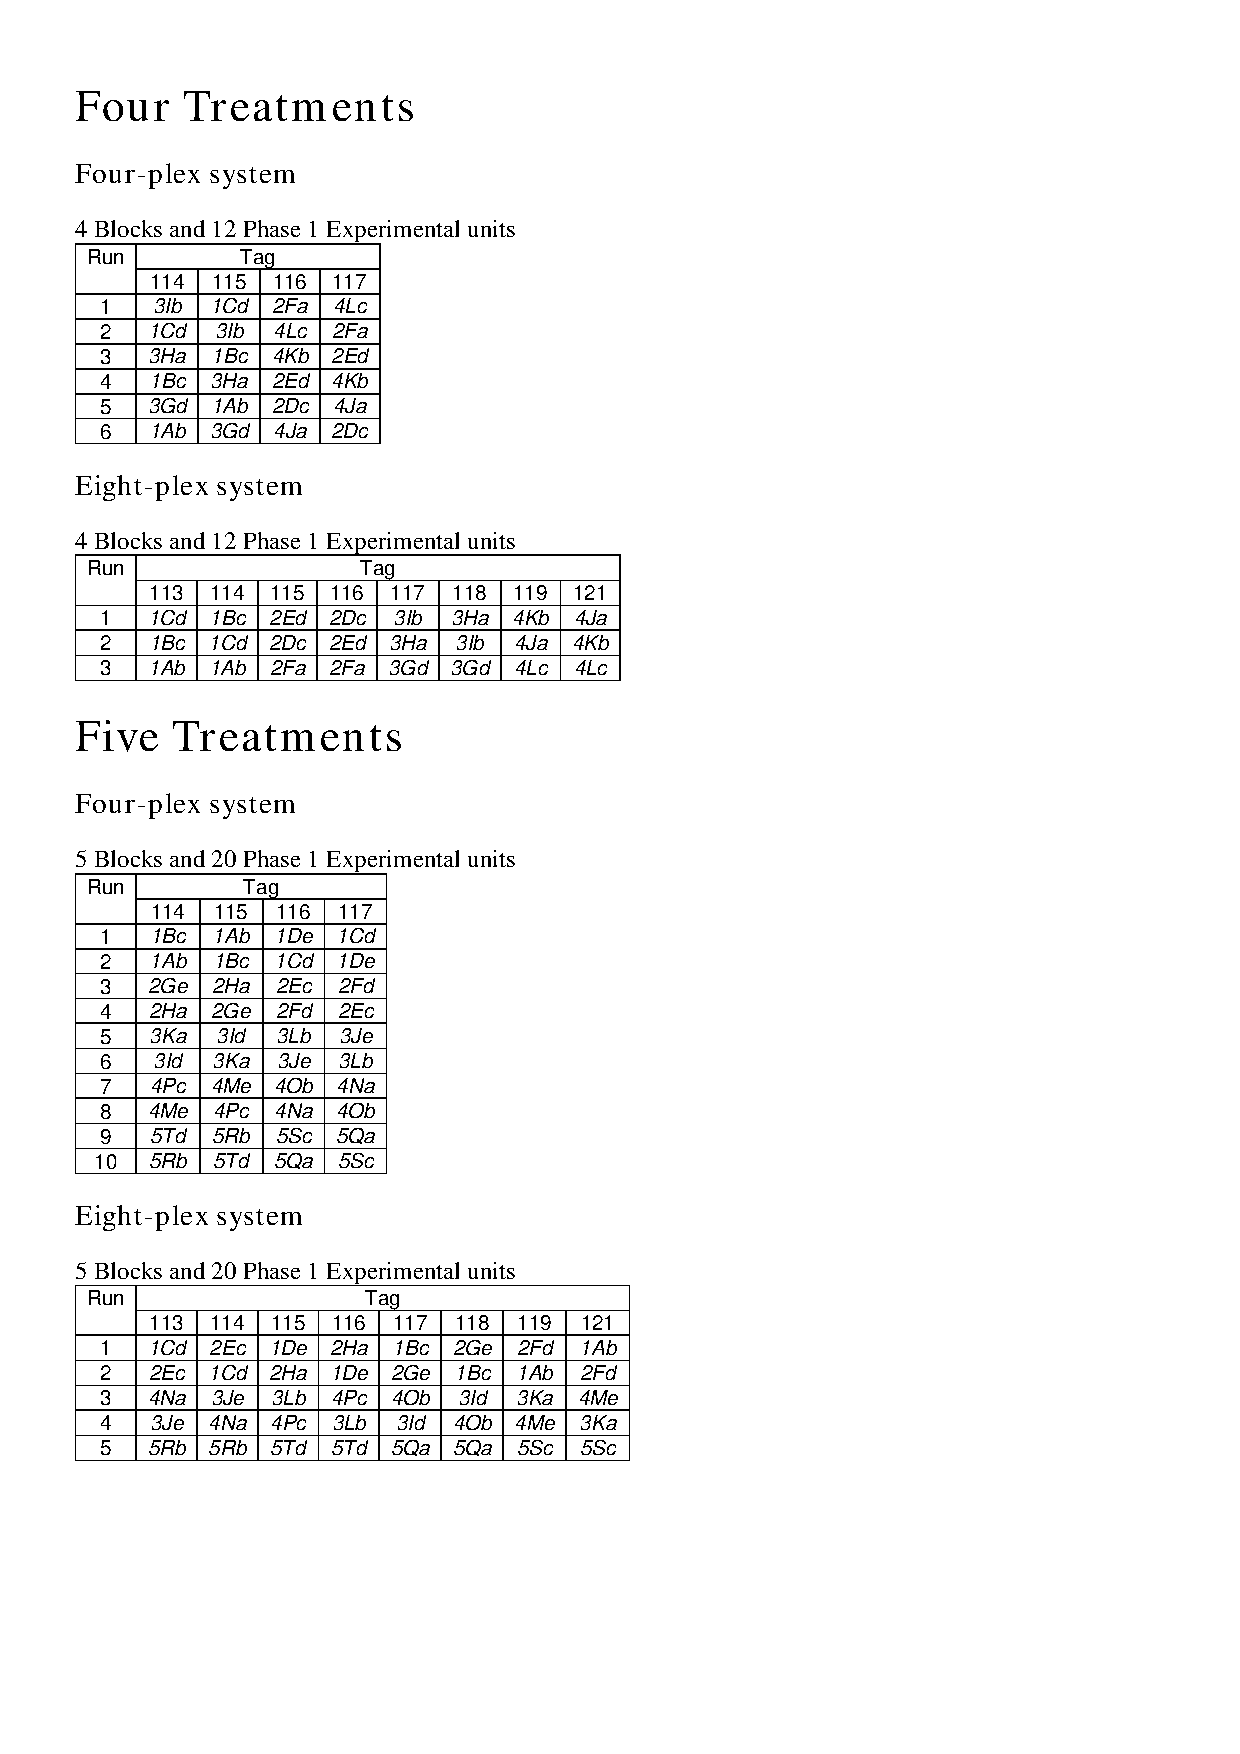
\includepdf[pages={1-},scale=1]{ChapterAppendix/BIBDdesigns.pdf}

\chapter{Tables of properties of optimal designs when Phase 1 is a BIBD} \label{append:optimalBIBD}

\includepdf[pages={1-},scale=1, fitpaper, rotateoversize]{ChapterAppendix/optimalBIBD.pdf}



\end{appendices}


\bibliography{ref}
\addcontentsline{toc}{chapter}{Bibliography}


\end{document}
